\documentclass[a4paper,12pt]{article}

% List of packages and custom commands/environments
\usepackage{amsmath,amssymb,amscd}
\usepackage[hidelinks]{hyperref}
\usepackage{dirtree}
\usepackage{tikz}
\usetikzlibrary{calc}
\usepackage{graphicx}
% \usepackage{subfig}
\usepackage{comment}
\usepackage{mathtools}
\usepackage{amsmath}
\usepackage{braket}
\usepackage{multirow}
%\usepackage[inline]{showlabels}
\usepackage{adjustbox}
\usepackage{caption}
\usepackage{subcaption}
\captionsetup{font=footnotesize}
\usepackage[a4paper,margin=2cm, marginparwidth=2cm]{geometry}
\usepackage{float}
\providecommand{\href}[2]{\code{#2}}
\providecommand{\url}[1]{\code{#1}}
\usepackage{bm}
\usepackage[a4paper,margin=2cm, marginparwidth=2cm]{geometry}

\usepackage{adjustbox}


\newcommand{\code}[1]{\mbox{%
        \ttfamily
        \tikz \node[anchor=base,fill=black!12]{#1};%
    }}

    \begin{document}
    \pagenumbering{arabic}
    \newgeometry{left = 1.75cm, right = 1.75cm, top = 1.75cm, bottom = 2cm}
    
    \vspace*{3cm}
    
    \begin{center}
     {\Large MPhil Data Intensive Science}  \\ [3pt]
     {\Large University of Cambridge}  \\ [3pt]
     
     \vspace*{1cm}
     \hrulefill
     \vspace*{0.75cm}
     
     {\LARGE \textbf{AstroCLIP: Cross-Modal Pre-training for Astronomical Foundation Models}} \\ [6pt]
     \large \textbf{Data Analysis Project} \\ [6pt]
     \vspace*{0.05cm}
     \hrulefill
     \vspace*{1.5cm}

     % Add the university logo here
    
\includegraphics[width=0.3\textwidth]{../figures/University_Crest.pdf} 

    \vspace*{1.5cm}
     
     {\Large  Andreas Vrikkis} \\ [6pt]
     {\large  December 14, 2023} \\ [3pt]
     {\large  \LaTeX \hspace{0.03cm} Word count:  } \\ [3pt]
     
     \end{center}   
    
    
    \newpage
    
    \restoregeometry
    
    \newpage
    
    \tableofcontents
    
    \newpage
\section{Introduction}

\section{Method/Background/Theory}
\subsection{Foundational Models}
\subsection{Self-Supervised Learning}
When labelled training data are scarce, other datasets can be exploited to improve performance. In \emph{transfer learning} a model is first pre-trained to perform a related secondary task for which we have (potentially labelled) data \cite{udl}. The resulting network is then adapted to the primary task of interest. This is typically done by removing the final layer(s) of the network and adding new layers (heads) that produce the desired output. Further training is then performed on the primary task. The pre-trained part of the network can be frozen (i.e. its weights are not updated during training) or it can be fine-tuned. 

The key principle behind this approach is that the pre-trained model has built a good internal representation of the data from the secondary task, which can be useful for the primary task. It can also be seen as a form of sensible weight initialisation for most of the final network.

For transfer learning to be effective, the secondary task should contain a large amount of data. In many cases, however, labelled data are scarce or expensive to obtain. In self-supervised learning (SSL), a model is trained on a pretext task where the labels are generated from the data itself. In the process, the model learns to extract rich, low-dimensional representations from data without the need for human labelling. The pretext task is often chosen to be an artificial surrogate task on the input data. Recently, numerous such tasks have been developed, including autoregressive prediction of the next word in a sequence \cite{radford2019language}, masked language modelling \cite{devlin2018bert} and contrastive learning \cite{radford2021learning}. These techniques have shown success in generating versatile and informative representations across NLP and computer vision.




\subsection{Cross-modal Constrastive Learning}
Constastive learning is a self-supervised learning technique.
The key concept behind our training objective is that different observational modalities represent correlated transformations of the same underlying physical object, forming a positive pair. By modality we refer to the type of data input such as iamges, text, etc. each requring a different processing technique. This is an extension of the single-modal contrastive learning framework such as SimCLR [cite], which employs stochastic data augmentation to create two views from the underlying image. Instead, we begin with two different modalities in different spaces and map them to a common embedding space, similar to the cross-modal framework connecting language and images in Ref.\cite{crossCLIP}. Under the constrastive loss function, each positive pair is projected together in the embedding space, while negative pairs are pushed apart.  

The cross-modal contrastive learning framework is illustrated in Fig.\ref{fig:contrastive_learning}. Here, $\mathbf{x}_i \in \mathbb{R}^N$ and $\mathbf{y}_i \in \mathbb{R}^M$ are two modalities of the same underlying object. These are passed through a pair of encoder networks $f_{\mathbf{\theta}}: \mathbb{R^N} \rightarrow \mathbb{R^D}$ and $g_{\mathbf{\phi}}: \mathbb{R^M} \rightarrow \mathbb{R^D}$, with $\mathbf{\theta}, \mathbf{\phi}$ trainable parameters, which extract representation vectors in the shared embedding space where contrastive loss is applied. These are denoted as $\mathbf{z}^x_i \in \mathbb{R}^D$ and $\mathbf{z}^y_i \in \mathbb{R}^D$, where $D$ is the dimensionality of the embedding space and the superscripts $x$ and $y$ denote the originator modality. 

\begin{figure}[H]
    \centering
    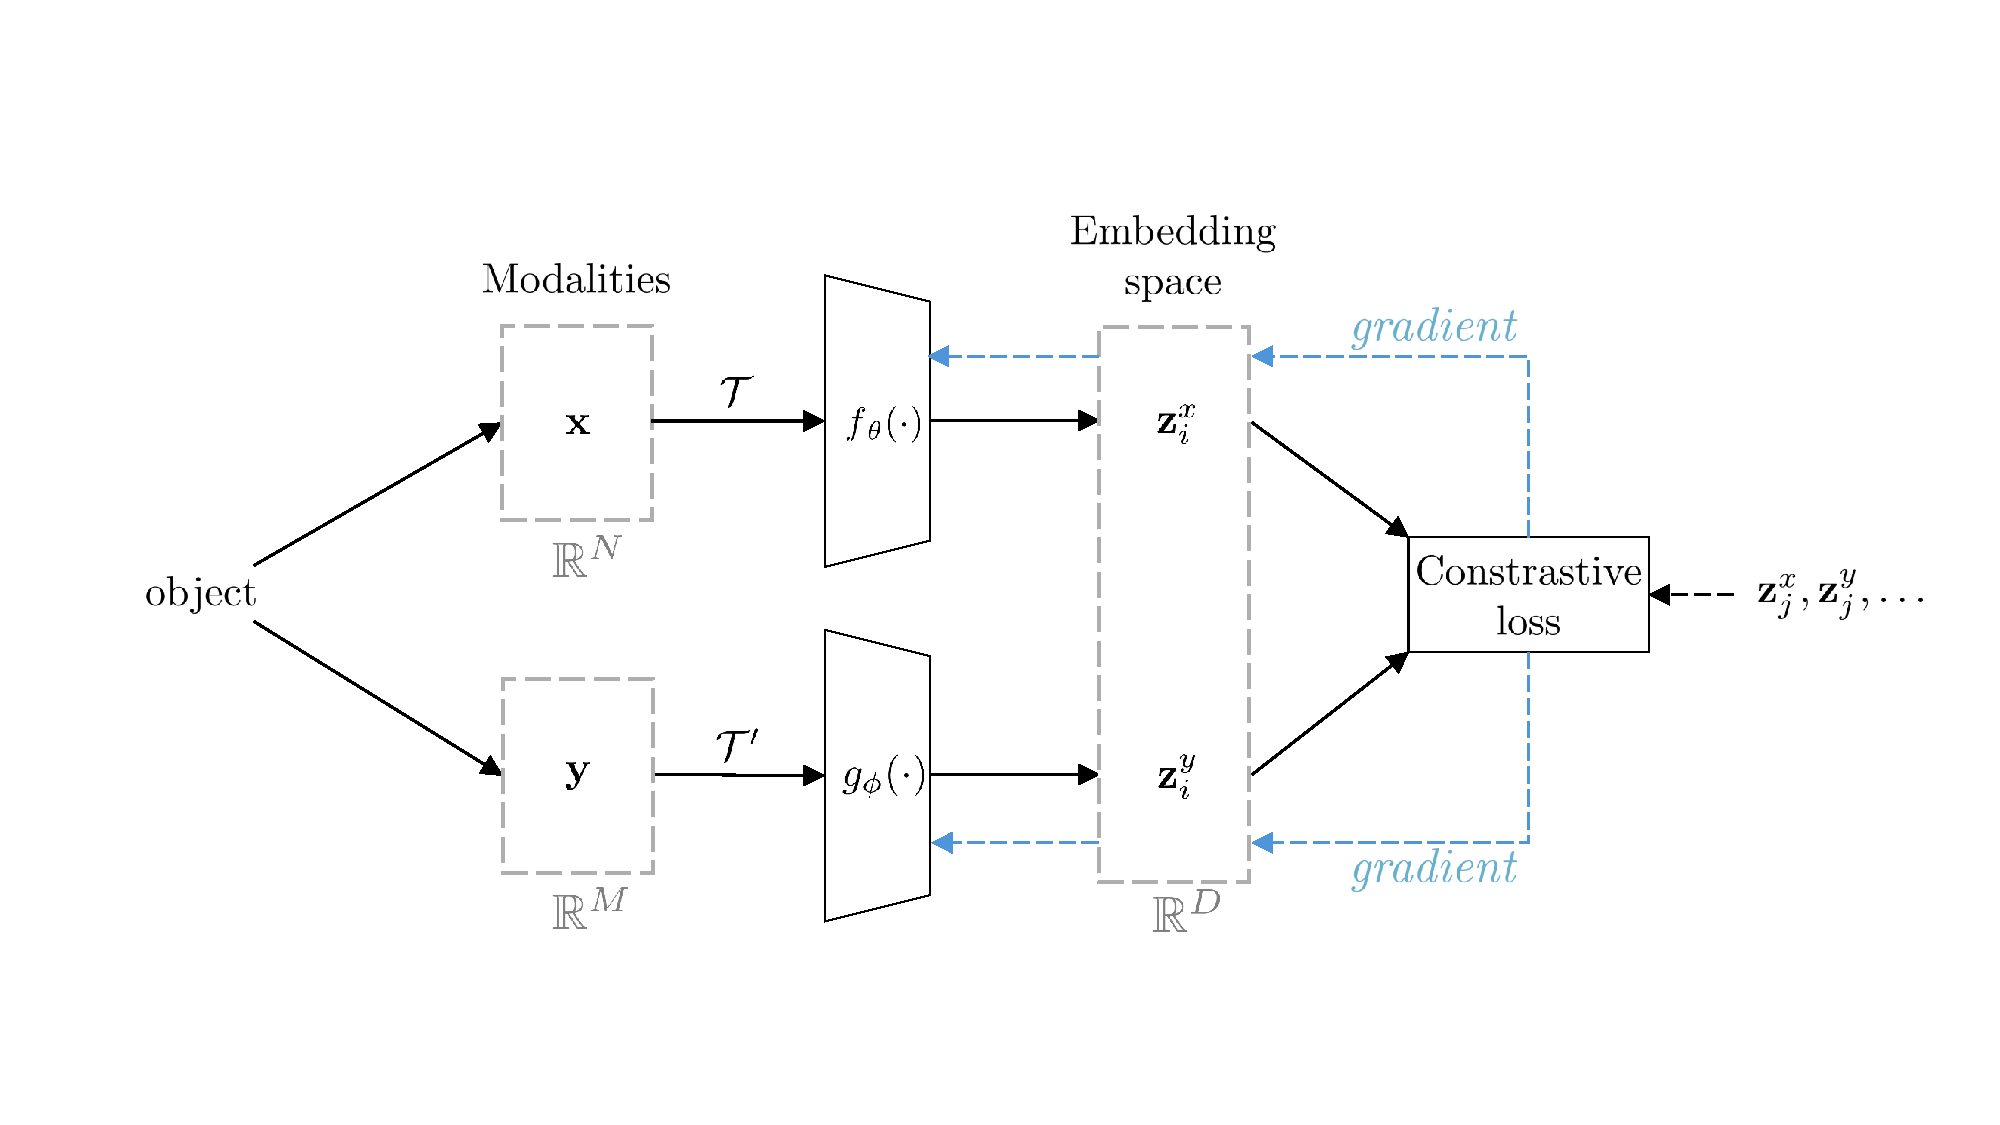
\includegraphics[width=\textwidth]{../figures/contrastive_learning.pdf}
    \caption{Cross-modal contrastive learning framework. An underlying physical object is observed in two different modalities, $\mathbf{x}_i \in \mathbb{R^N}$ and $\mathbf{y}_i \in \mathbb{R^M}$. An augmented version of each modality undergoes a transformation $\mathcal{T}, \mathcal{T}'$ and are passed through encoder networks $f_{\theta}, g_{\phi}$ which compress them into representations $\mathbf{z}^x_i, \mathbf{z}^y_i$ in a shared embedding space. The constrastive loss (InfoNCE) is applied to these representations along with the negative pair denoted by $j$, with the gradients backpropagated to update the encoder networks (appended with projection heads).}
    \label{fig:contrastive_learning}
\end{figure}


We want this embedding space to maximise the mutual information $I(f_{\theta}(\mathbf{x}),g_\phi{\mathbf{y}})$ between these two representations. However, calculating the mutual information directly is intractable for finite data \cite{mutualinfolimitation}. Instead, we approximate each modality as a noisy transformation of the same underlying object and use an Information Noise-Contrastive Estimation (InfoNCE) loss function \cite{infonce} which maximises a variational bound on the mutual information. The InfoNCE loss is defined as:

\begin{equation}
    \mathcal{L}_{\text{InfoNCE}}(\mathbf{z}^x, \mathbf{z}^y, \tau) = -\frac{1}{K} \sum_{i=1}^{K} \log \frac{\exp\left(S_C(\mathbf{z}^x_i, \mathbf{z}^y_i)/\tau\right)}{\sum_{j}^{K} \exp\left(S_C(\mathbf{z}^x_i, \mathbf{z}^y_j)/\tau\right)}
    \label{eq:infonce}
\end{equation}
where $\mathbf{z}^x_i=f(\mathbf{x}_i)$ and $\mathbf{z}^y_i=g(\mathbf{y}_i)$, $\tau > 0$ denotes a smoothing parameter (referred to as temperature) , $S_C(\mathbf{z}^x_i, \mathbf{z}^y_i)$ is a similarity metric between the two representations, and $j$ represent the indices of negative examples (i.e representations of different objects to object $i$). For the similarity metric in CLIP, we use the cosine similarity between the two representations in the embedding space given by:
\begin{equation}
    S_C(\mathbf{z}^x_i, \mathbf{z}^y_j) = \frac{(\mathbf{z}^x_i)^T \mathbf{z}^y_j}{\|\mathbf{z}^x_i\|^2 \|\mathbf{z}^y_j\|^2}.
    \label{eq:cosine}
\end{equation}
InfoNCE is biased, but it represents a stable, low variance bound on the mutual information that is widely used in constrastive methods \cite{crossCLIP}. Under InfoNCE, points in the embedding space that correspond to the same object are pulled together, while points that correspod to different objects are pushed apart.

Training cross-modal models from scratch under CLIP loss on cross-modal problems has been shown to often underperform compared to single-modal problems. However, the addition of pre-trained single modal models as initialisation can significantly improve performance. This is the approach taken in this project, where only an additional projection head is trained on top of the pre-trained models.



\subsection{Embedding Space}
The low-dimensional, rich representations of the data in the shared embedding space can then be used for a variety of downstream tasks. It has been shown in various contexts that despite the contrived training objective, the embedding space can capture a significant amount of semantic information that often outperform supervised training on zero-shot and few-shot learning tasks. Recall that during constrastive training, the embedding space structures itself such that semantically similar objects are close together, while semantically dissimilar objects are far apart. 
This means that the positions of the representations in the embedding space can be used to infer semantic relationships between the objects and can be used for downstream tasks. A typical way of visualising the embedding space is to project the representations to a 2D space using dimensionality reduction techniques. 

UMAP (Uniform Manifold Approximation and Projection) is a dimensionality reduction technique that aims to preserve the global structure and local relationships of data when mapping high-dimensional data to a lower-dimensional space \cite{UMAP}. UMAP constructs a high-dimensional graph representation of the data, which it then optimises to create a low-dimensional projection that maintains as much of the original data's structure as possible. 

As the embedding space structure is informed by the contrastive loss, the arrangment of the representations holds semantic information. Island structures in the embedding space can be interpreted as clusters of semantically similar objects, while the distance between islands can be used to infer semantic relationships between the clusters.


\section{Implementation}
In AstroCLIP, we consider two modalities of galaxies: images and spectra. In essence, we approach the two modalities as filtered, noisy views of the same underlying galaxy. This implies that they should possess a shared latent space in which the embeddings of these cross-modal representations are aligned. To obtain these embeddings, we deploy a pair of models to encode the images and spectra. This is done in a two-step process:
\begin{enumerate}
    \item We utilise two pre-trained single-modal models, one for images and one for spectra, which were pre-trained using SSL. For the pretrained image embedder, we use a galaxy image encoder from Stein et. al (see Ref.\cite{stein}), which is based on MoCo v2 \cite{mocov2}. For galaxy spectra, we utilise the encoder part from the Spender model \cite{spender}.
    \item We append a simple Multilayer Perceptron (MLP) projection head to each of the pre-trained models to compress the representations into a shared $d=128$-dimensional embedding space. We then train (or fine-tune) these projection heads under constrastive learning to align the embedded representations of the two modalities under shared semantics.
\end{enumerate}
We keep the pre-train single-modal models frozen during training, only updating the projection heads, instead of training the entire model from scratch. This is to align with the previous studies that show that pre-training the single-modal models significantly improves performance in cross-modal tasks \cite{crossCLIP}.

We note here the deviation from the original AstroCLIP paper (v1): in the original papers, the authors pre-train a transformer model, structured similar to GPT-2, to embed the spectra. This is a much larger model than Spender, totalling around 43.2M parameters. However, the transformer model is not publicly available, and the authors do not provide details on the pre-training process. Instead, we opt to use the Spender model based on the suggestion of one of the authors. We provide details of 
the two models, the data used and the training process in the following sections.



\subsection{Data}
\label{sec:data}
\subsubsection*{DESI Legacy Survey Images}
We use the same data as the original AstroCLIP paper (v1). For galaxy images, we sue the DESI Legacy Survey Data Release 9 imaging data from January 2021 \cite{DESI} as prepared by Stein et. al \cite{stein}. The $g$ and $r$ band data for the northern galactic cap (NGC) were captured by the Beijing-Arizona Sky Survey, while the $z$ band data came from the Mayall Legacy Survey. For the southern galactic cap (SGC), the data were collected by the Dark Energy Camera Legacy Survey (DECaLS). We filter out the images that were identified as stars by the Legacy Survey team and impose a mag$_z$ cutoff for $z$-bands above 20. This corresponds to an initial dataset of 41M (g,r,z) images of size $152 \times 152$, which we centre-crop to $96 \times 96$ for training. The cropping is done as the great majority of galaxies cover less area than the total size of the image and thus often include overlaping regions of the sky.

\subsubsection*{DESI Spectra}
To pair the images with spectra, we cross-match the galaxy spectra from the DESI Early Data Release \cite{DESI2023}, which contains spectra observed by the Survery Validation compaign. This cross-match is done using the target IDs associated with each galaxy. This results in total subset of 197,976 pairs of images and spectra. During the training process, we Z-score normalise each individual spectrum to have zero mean and unit variance. We then split the data into training and validation sets, with 90\% of the data used for training and 10\% for validation.

\subsubsection*{Data Catalogue for Downstream Tasks}
For experiments involving the prediction of physical properties from the embeddings, we further cross-match the image-spectrum pairs with the PRObabilistic Value-Added Bright Galaxy Survery (PROVABGS) catalogue \cite{PROVABGS}. We then specifically extract the estimates of the redshift ($\mathcal{Z}$) and stellar mass ($M_{\star}$) for each galaxy ID that is present in the catalogue. We then perform the same filtering process as the original AstroCLIP paper: we only select enetries for which $M_{\star} > 0$ and mag$_g$,mag$_r$,mag$_z$ $> 0$, removing spurious entries. This yields a total of 105,159 entries, which we split into training and validation using a 90/10 ratio.



\subsection{Pre-trained Image Embedder} 
The pre-trained image embedder we used in this reconstruction was developed by Stein et. al. (2021a) \cite{stein}. It is based on the MoCo v2 framework \cite{mocov2}, and it uses a ResNet-50 backbone as the encoder network. The model was pre-trained on a curated subset of 3.5M galaxies sampled uniformly by $z$-bands magnitude from the DESI Legacy Survey. They authors use a single-modal contrastive learning SSL framework, where each image undergoes multiple stochastic augmentations to create two views of the same image. The augmentations include galactic extinction, random cropping, random rotation, size scaling, point-spread function blur, jittering and Gaussian noise addition. The model was then trained on a contrastive loss function to align the representations of the two views in the embedding space. 

\begin{figure}[H]
    \centering
    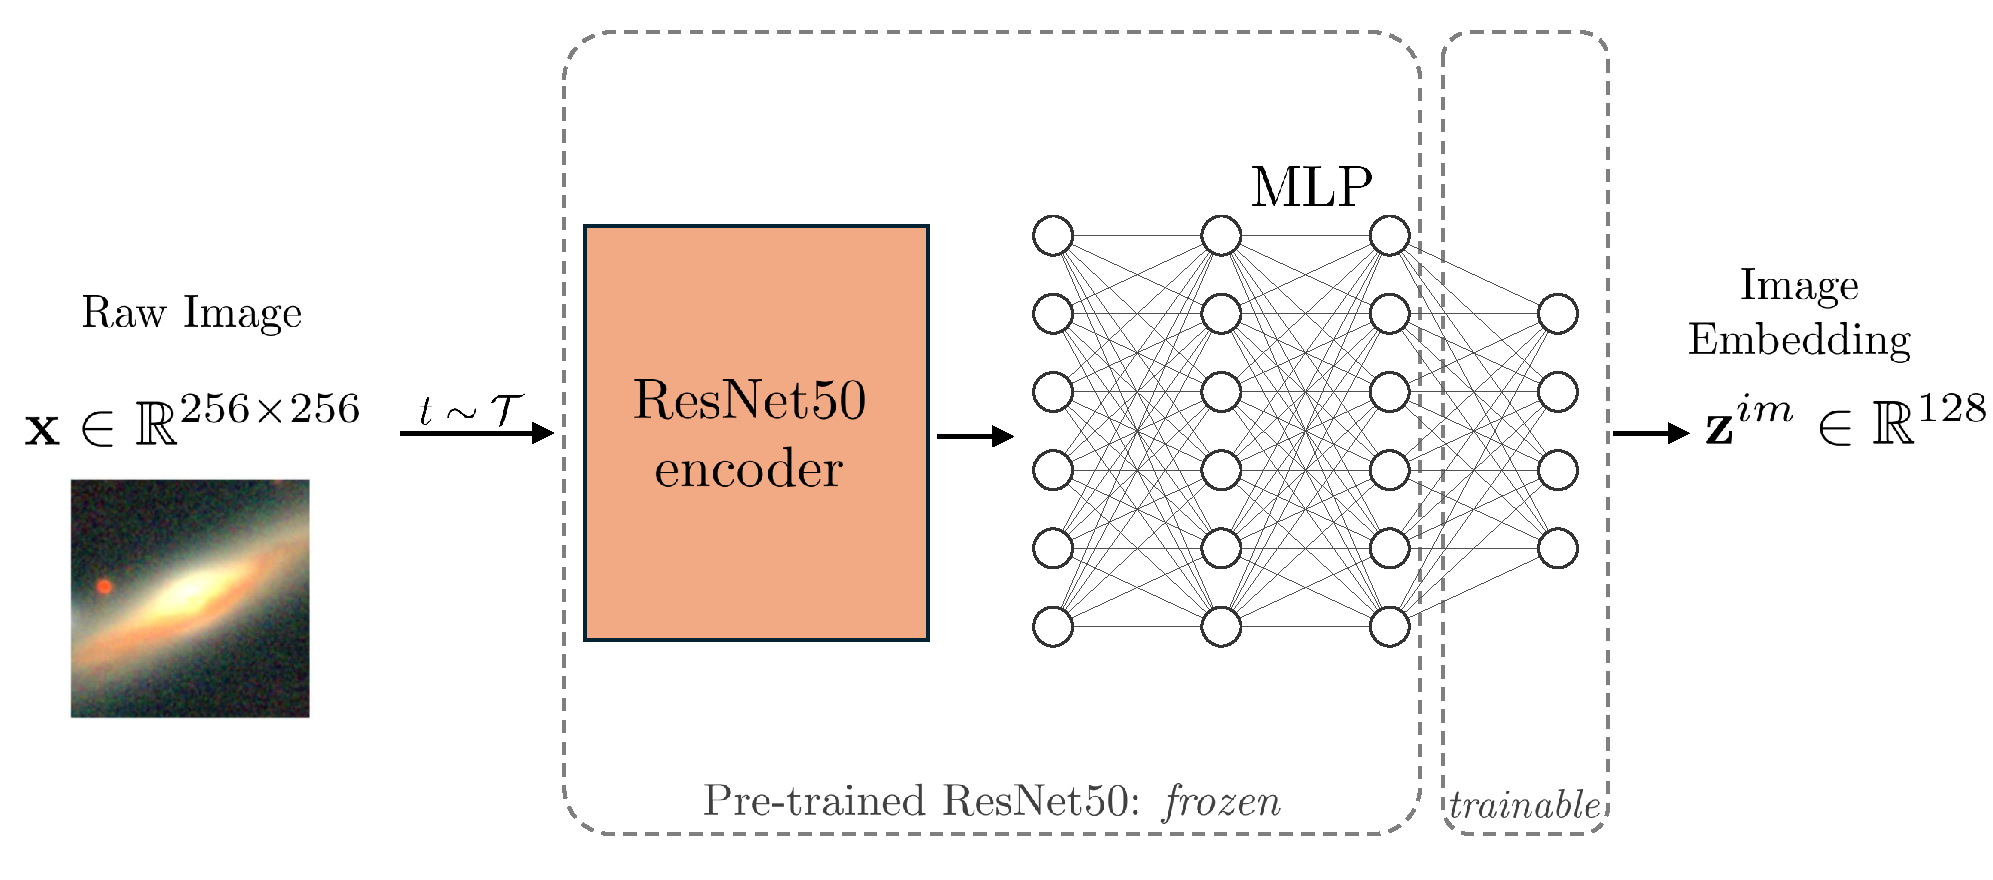
\includegraphics[width=\textwidth]{../figures/diagram_resnet.pdf}
    \caption{Diagram ResNet50.}
\end{figure}

The model is publicly available and can be downloaded from the authors' GitHub repository. This model has 50 ResNet blocks that contain a batch normalisation opeartoin, followed by an activation function and a convolutional layer. It has a total of 28M parameters. We keep the convolutional layers frozen during constrastive training, and use the final fully connected layer as the trainable projection head. This amounts to 4.5M trainable parameters that are finetuned under InfoNCE loss. 


\subsection{Pre-trained Spectrum Embedder}


\begin{figure}[H]
    \centering
    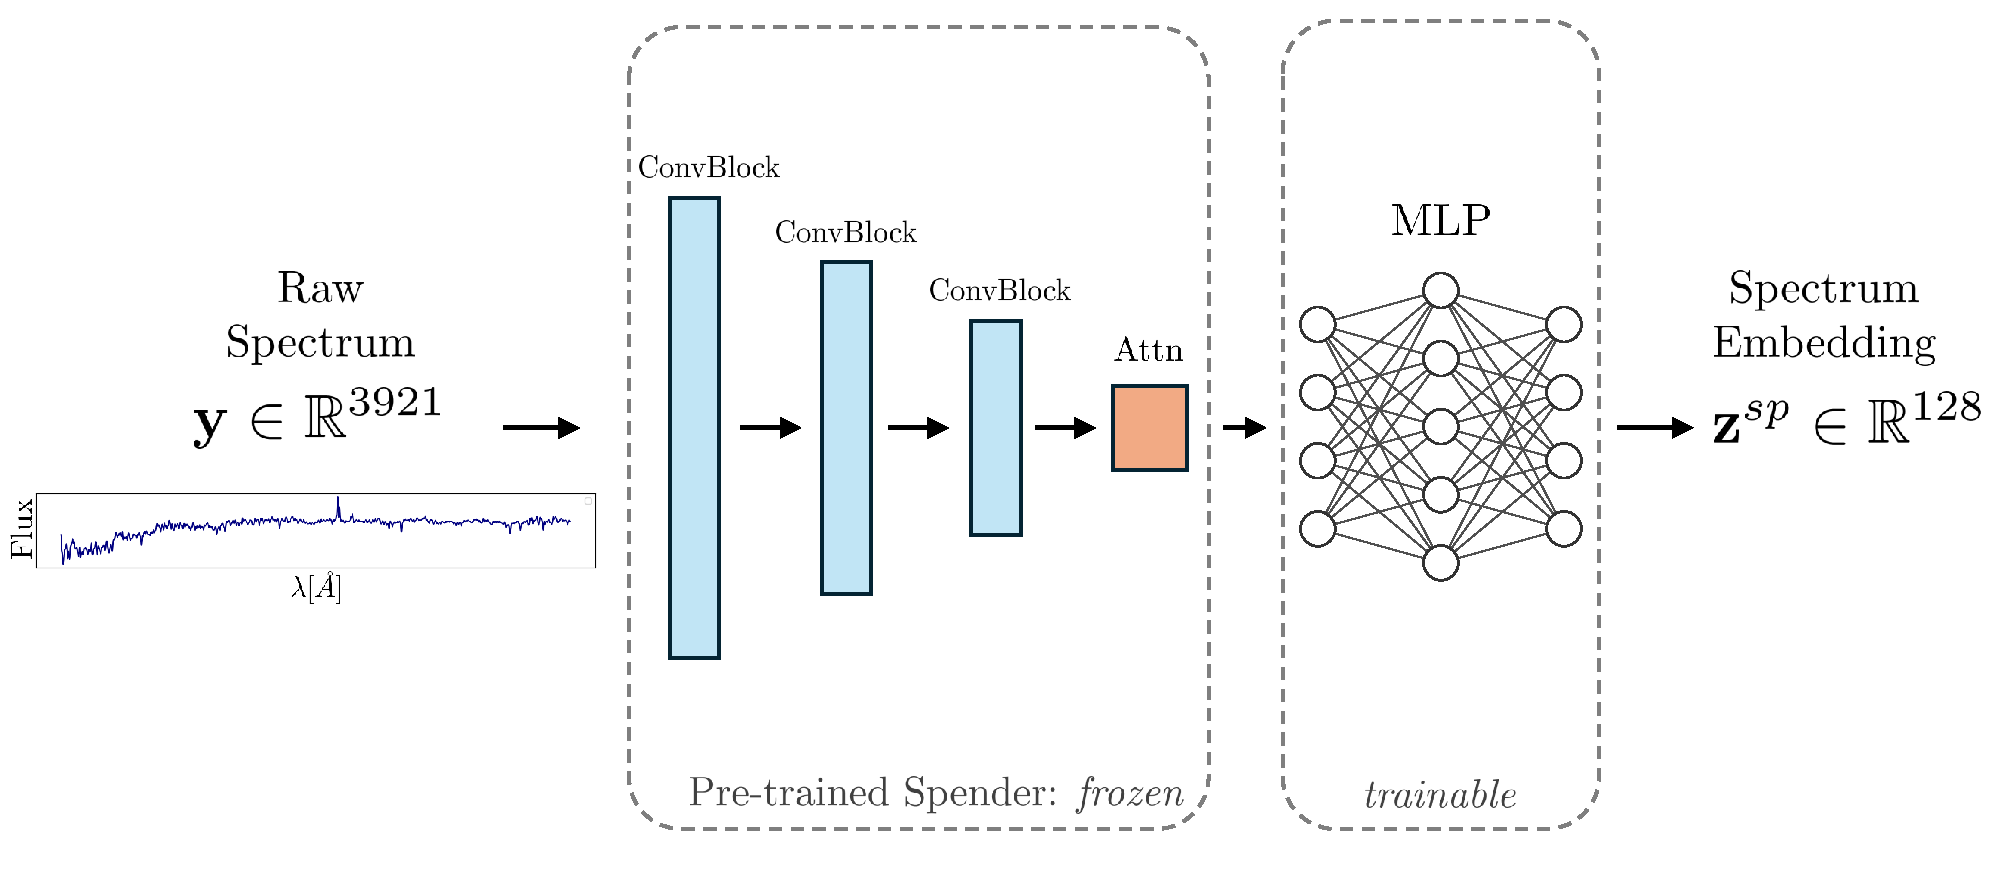
\includegraphics[width=\textwidth]{../figures/diagram_spender_cropped.pdf} % 1.3x text width to extend into the margins
    \caption{The }
    \label{fig:spender}
\end{figure}


We choose to use the Spender model \cite{spender}, an autoencoder network, to extract latent parameters from the observed spectra. The encoder part of the network consists of three convolutional layers with progressively wider kernel sizes (5, 11, 21), each followed by a trainable PReLU activation function and max-pooling. This translates the $M=3921$ spectral components into 512 channels for 72 wavelength segments. The model then applies attention by splitting the channels into two: $\mathbf{h}$ and $\mathbf{k}$, each of 
dimension $256 \times 72$. It then combines these channels as follows:

\begin{equation}
    \mathbf{e} = \mathbf{h} \cdot \text{softmax}(\mathbf{k}) \equiv \mathbf{h} \cdot \mathbf{a},
\end{equation}
where the dot product and the softmax are applied on the last dimension, denoting the wavelength. The attention weights in vector $\mathbf{a}$ indicate the presence and location of relevant signals, allowing the corresponding values to be enhanced into the attended features $\mathbf{e}$. This approach efficiently accommodates the apparent shift of spectral features in galaxies at varying redshifts. These are then fed into a series of fully connected layers to compress the representation into a $s=6$ dimensional latent space. These are then fed into the decoder part of the network which reconstructs the original spectrum. As usual in autoencoder networks, it is trained end-to-end with an MSE loss function. 

For AstroCLIP, we throw away the decoder part of the network, and use the convolutional layers and attention mechanism of the encoder. We replace the MLP which was used to compress the representation into a 6-dimensional latent space with a new fully connected MLP with 3 hidden layers of size 256, 128, 128 and a final output layer of size $d=128$ with ReLU activation functions. This is then trained under the InfoNCE loss function, while the convolutional layers and attention mechanism are kept frozen. The frozen layers contain semantic information about the spectra that is useful to incorporate through transfer learning. Overall, this amounts to [fix] trainable parameters, two orders of magnitude less than the original AstroCLIP encoder (4.5M parameters) \cite{astroclip}. 


\subsection{Constrastive Training}
The pre-trained models form parts of our unified AstroCLIP model. We then train both models under InfoNCE loss defined in eq.(\ref{eq:infonce}). The embedded representations that originate from the same galaxy are considered positive pairs, with all other considered negative pairs. Before an image is passed through the image embedder, we apply basic augementations in the following manner: a fixed crop to the central $96 \times 96$ pixels, random roation, random horizontal flip and gaussian blur. We set the batch size to $K=512$ image-spectrum pairs, as it was shown in Ref.\cite{radford2021learning} that larger batch sizes often correlate with better performance. We train the models using the Adam optimiser \cite{adam} for 80 epochs on a single NVIDIA A100-SXM-80GB GPU on the Camridge Wilkes3 cluster. We use an adaptable learning rate scheduler that reduces the learning rate by a factor of 2 (chosen by trial and error) if the validation loss does not improve for 5 epochs, using \verb|PyTorch|'s \verb|ReduceLROnPlateau| \cite{LRon}. Similar to the results observed in other studies such as Ref.\cite{gir},  our performance improves when we keep the temperature parameter $\tau$ constant rather than allowing it to vary. The training process takes roughly 2 hours to complete.

\subsection{Downstream Tasks}
To demonstrate the capabilities of AstroCLIP's embedding space, we demonstrate its performance across a range of tasks for which it was not explicitly trained for, nor fine-tuned. We firstly embed all galaxy image and spectra in the validation set (obtained as outlined in section \ref{sec:data}) using the trained AstroCLIP model as follows:

\begin{equation}
    \text{Initial Modality representation} : \left( \mathbf{x}^{\text{im}}, \mathbf{x}^{\text{sp}} \right) \xmapsto{\text{AstroCLIP}} \text{Embeddings} : \left( \mathbf{z}^{\text{im}}, \mathbf{z}^{\text{sp}} \right) \in \mathbb{R}^{128}.
\end{equation}
We then normalise both image and spectrum embeddings as:
\begin{equation}
    \mathbf{\bar{z}}^{im} =  \frac{\mathbf{z}^{im} }{|| \mathbf{z}^{im} ||_2}, \quad \mathbf{\bar{z}}^{sp} =  \frac{\mathbf{z}^{sp} }{|| \mathbf{z}^{sp} ||_2}.
\end{equation}
and use the normalised galaxy embeddings in a shared, cross-modal latent space to perform the tasks outlined below.

\subsubsection*{Query Retrieval}
We showcase the architecture's ability to align embeddings of galaxies, we choose a random galaxy from the validation set and retrieve similar galaxies purely based on the embedding space structure. Specifically, we perform the galaxy search using the cosine-similarity (eq.(\ref{eq:cosine})) between the query galaxy $\bar{\mathbf{z}}_q$ and all other galaxies in the validation set. We then rank the galaxies based on the similarity score and display the top 5 most similar galaxies. For instance, to search for galaxy images that correspond to a specific query spectrum $\mathbf{y}_i$, we calculate the cosine similarity between the query spectrum embedding $\{\mathbf{x}^{sp}_i\}_{val}$ and the image embeddings $\{\mathbf{x}^{im}_i\}_{val}$ in the validation set. The target images with the highest similarity values are then returned. This process requires no additional transformations or alterations.

This allows us to search the embedding space for both the image and spectrum embeddings, which is unique to this cross-modal framework. We present examples for both \emph{in-modality} $S_{C}(\mathbf{z}^{im}_q, \mathbf{z}^{im}_j)$ or $S_{C}(\mathbf{z}^{sp}_q, \mathbf{z}^{sp}_j)$, where the query and target embeddings are of the same modality, and \emph{cross-modality} $S_{C}(\mathbf{z}^{im}_q, \mathbf{z}^{sp}_j)$ or $S_{C}(\mathbf{z}^{sp}_q, \mathbf{z}^{im}_j)$, where the query and target embeddings are of different modalities.







\subsubsection*{Zero Shot Prediction of Physical Properties}
To evaluate AstroCLIP's ability to predict physical properties of galaxies, we consider the task of predicting the catalogue-based redshift $\mathcal{Z}$ and stellar mass $M_{\star}$ of galaxies from the embedded galaxy representations. Each of the embeddings has a corresponding redshift and stellar mass value provided by the PROVABGS catalogue. These values are used as the ground truth for the prediction task, but note that they were not used in the training process. We then proceed by performing a simple $k$-Nearest Neighbour ($k$-NN) regression on the embedded representations to predict the redshift and stellar mass values. 
%We use simple $k$-Nearest Neighbour ($k$-NN) our embedded images and spectra to predict the physical properties without any additional training or finetuning.  
We do this by further splitting the 30K pairs in the validation set into a training and held-out test set. We then train a $k$-NN regressor on the new training set and evaluate its performance on the test set. We then instantiate the $KNeighborsRegressor$ with parameters set to \texttt{weights="distance"} and \texttt{n\_neighbors=16}. By setting \texttt{weights} to \texttt{"distance"}, the algorithm ensures that closer neighbors have a greater influence on the prediction, as their contributions are inversely proportional to their distances from the query point. This method allows us to calculate the predicted values for redshift and stellar mass as weighted averages of the target values of these nearest neighbors. 

\subsubsection*{Embedding Space Analysis}
We analyse the embedding space structure by projecting the embeddings to a 2D space using UMAP \cite{UMAP}. By doing this for image embeddings in isolation, spectra embeddings in isolation and the combined image-spectrum embeddings, we showcase the ability of constrastive training to align the embeddings based on shared semantics. First, we want to examine whether the model is able to separate the galaxy embeddings based on particular characteristics. To that end, we look for look for isolated collections of galaxies in the embedding space, which we refer to as `islands'. We then examine the galaxies in these islands to see if they share any common characteristics. Secondly, we examine whether the model is able to create meaningful clusters in the high-dimensional embedding space, which may share common characteristics. As the embedding space structure is informed by both the image representations and the spectrum representations, we expect to see clusters which contain galaxies that are similar in both modalities.
To detect these islands on the 2D UMAP projection, we use the DBScan clustering algorithm \cite{dbscan} from \verb|scikit-learn|.DBSCAN (Density-Based Spatial Clustering of Applications with Noise) is an unsupervised machine learning algorithm designed to identify clusters in large spatial datasets by examining the local density of data points. The algorithm categorises points into core points, border points, and noise points, governed by two parameters: $\epsilon$ (epsilon) and $\text{minPts}$ (minimum points).

\begin{itemize}
    \item \textbf{Core Points:} A point is considered a core point if it has at least $\text{minPts}$ points within $\epsilon$ radius, including the point itself. This criterion ensures that core points are those with a high density of neighbouring points.

    \item \textbf{Border Points:} Border points are not core points but are located in the neighborhood of a core point. These points have fewer than $\text{minPts}$ within their $\epsilon$ neighborhood but are reachable from core points.

    \item \textbf{Noise Points:} Noise points are data points that are neither core points nor border points. These points do not belong to any cluster.
\end{itemize}
DBSCAN starts by arbitrarily selecting a point and assessing whether it is a core point. If it is, the algorithm then iteratively explores and includes all directly reachable points, thereby expanding the cluster. This process continues until no new points can be added to the cluster. Points that are reachable from a core point via other core points are also included in the same cluster.

An illustration of the DBSCAN algorithm is shown in Fig.\ref{fig:dbscan}. DBSCAN is particularly effective in identifying islands in 2D projections like UMAP because it clusters based on local density, allowing for the detection of irregularly shaped clusters without requiring predefined cluster numbers. 

\begin{figure}[H]
    \centering
    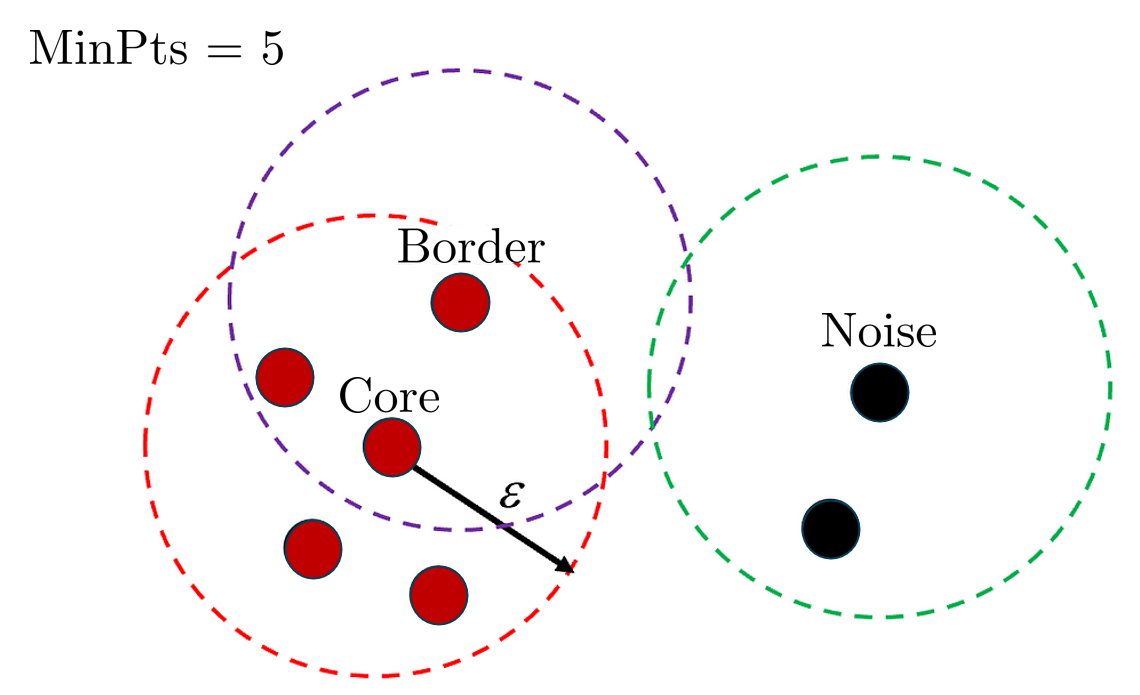
\includegraphics[width=0.5\textwidth]{../figures/dbscan_diagram.png}
    \caption{DBSCAN illustration: in this diagram, minPts = 5. 
    The red points form a cluster, with 4 core points because the area surrounding these points in an $\epsilon$ radius contain at least 5 points (including the point itself). A border point is also included in the red cluster because it is reachable from a core point. The black points are noise as they are neither core points nor directly-reachable.}
    \label{fig:dbscan}
\end{figure}

To cluster the high-dimensional embeddings ($d = 128$), we use k-Means \cite{udl} clustering from \verb|scikit-learn|. K-means is a centroid-based clustering algorithm that partitions a dataset into \( k \) clusters, where \( k \) is a user-specified parameter. The algorithm works by initialising \( k \) centroids, assigning each data point to the nearest centroid, and iteratively updating the centroids to minimise the variance within each cluster until convergence. We use the silhouette score \cite{silhouette} to evaluate the quality of the clustering, and we choose a reasonable value that balances the number of clusters and the quality of the clustering. We then project the embeddings to a 2D space using UMAP, and examine the spectra and images of the clusters formed.






%---------------------------------------
\section{Results}
In this section, we present our results from the AstroCLIP reproduction. Where appropriate, we compare our results to the original AstroCLIP paper (v1) \cite{astroclip} and discuss possible reasons for any discrepancies. A discussion on the implications of our results and potential future work is also provided.

\subsection{Loss Curves}
Fig.\ref{fig:loss} shows the average InfoNCE loss per epoch for training and validation sets during the constrastive training. We note here that validation loss in constrative learning is not a direct measure of performance, but rather a proxy for the model's generalisation ability, as the training does not involve any labelled data.
\begin{figure}[H]
    \centering
    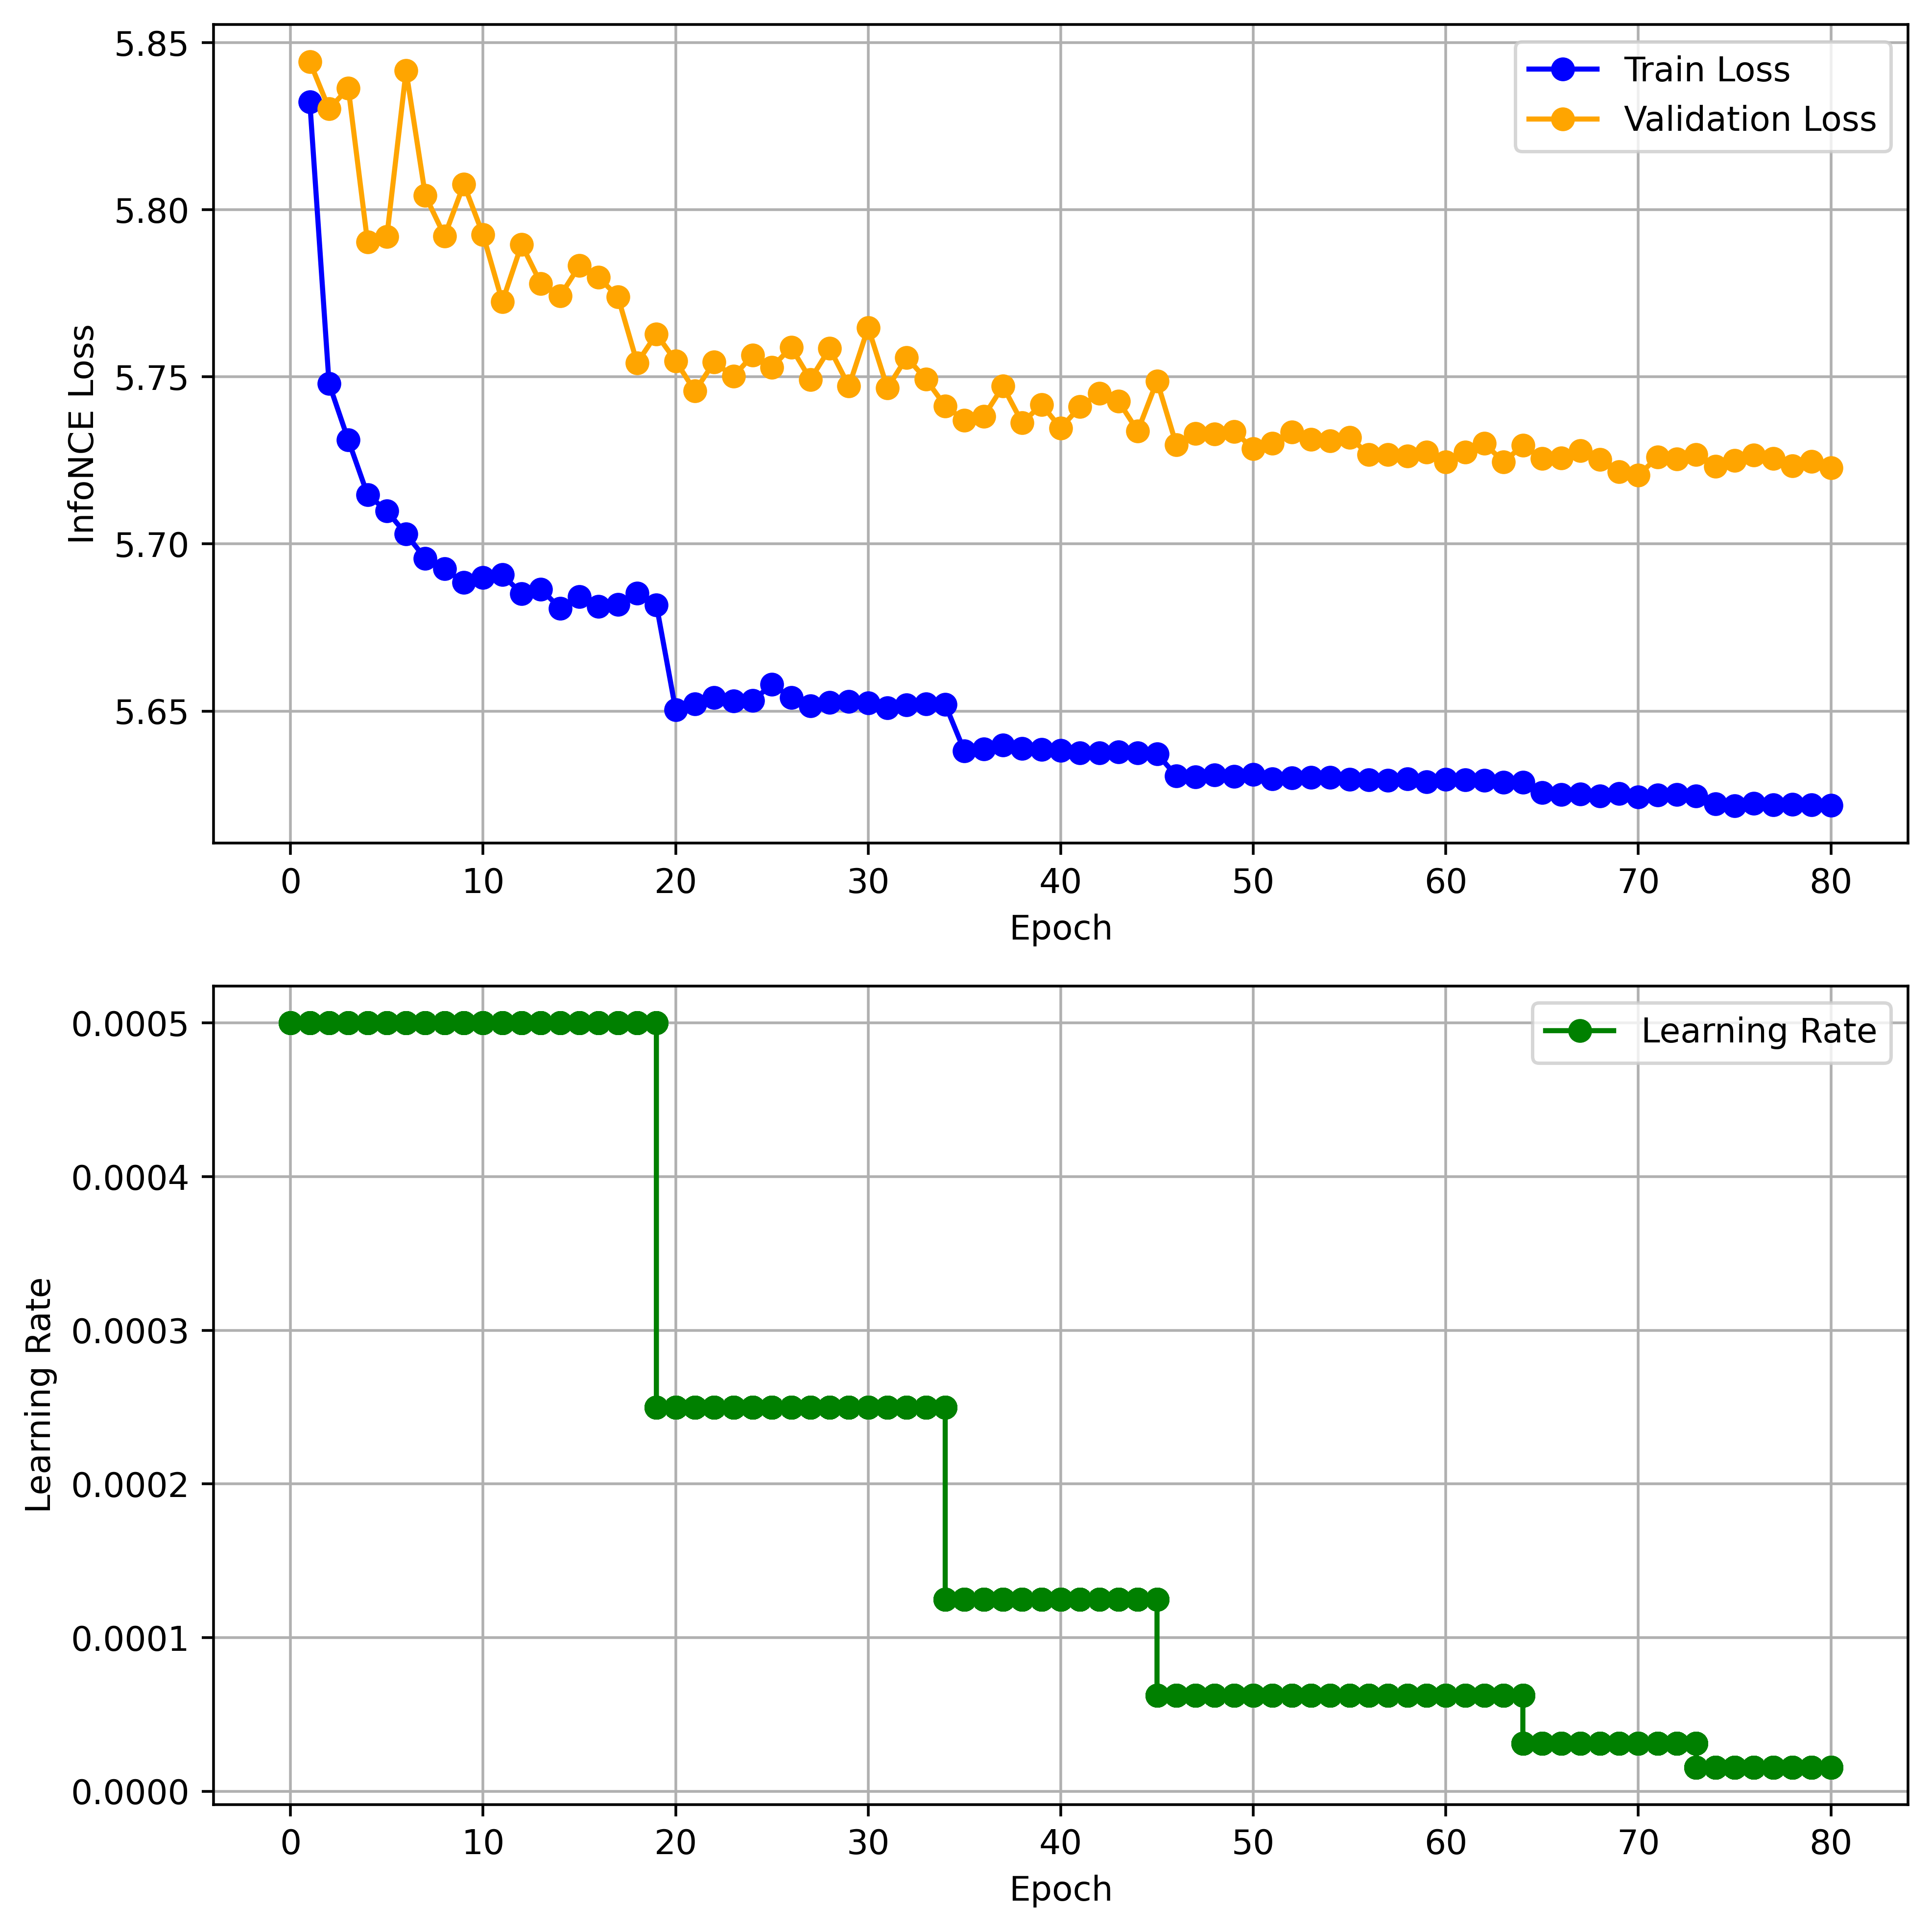
\includegraphics[width=0.8\textwidth]{../figures/training_plot.png}
    \caption{Average InfoNCE loss per epoch for training and validation sets during constrastive training (top), and the learning rate schedule (bottom). The learning rate is reduced by a factor of 2 if the validation loss does not improve for 5 epochs.}
    \label{fig:loss}
\end{figure}

Both the training and validation loss decrease steadily over the 80 epochs, indicating that the model is learning to align the image and spectrum embeddings in the shared latent space. The validation loss is consistently higher than the training loss as expected, but does not diverge significantly nor is starting to increase, indicating that the model is not overfitting. Whenever the training loss plateaus for 5 epochs, the learning rate is reduced by a factor of 2, which results in further decrease in the loss. The loss continues to decrease, albeit at a slower rate, until the end of the training. This could indicate that the model has not fully converged and could benefit from further training. 

The original work did not provide loss curves, learning rate nor the numbers of epochs, and so a direct comparison is not possible. 




\subsection{Query Retrieval}
We present the images of the four most similar galaxies (based on the cosine similarity of their embeddings) to four random query galaxy for all four possible combinations of modalities in Fig.\ref{fig:retrieval}. By construction, for in-modal searches the best match for the query galaxy is the galaxy itself, as the similarity score is 1.0. The model is able to retrieve galaxies that are visually similar to the query galaxy. The colour is well preserved in both in-modal and cross-modal searches, indicating that the model has learned to align the image and spectrum embeddings in the shared latent space. If the model was trained as a single-modal model, we would expect in-modal image searches to perform better than cross-modal searches. However, the model is able to retrieve visually similar galaxies in both cases, indicating that the both modality embeddings are informed by each other.  This is the reason why spectrum query - spectrum retrievals $S_C(\mathbf{z}^{sp}_q, \mathbf{z}^{sp}_j)$ are have similar images as well. 

\begin{figure}[H]
    \centering
    \begin{subfigure}{0.08\textwidth}
        \centering
        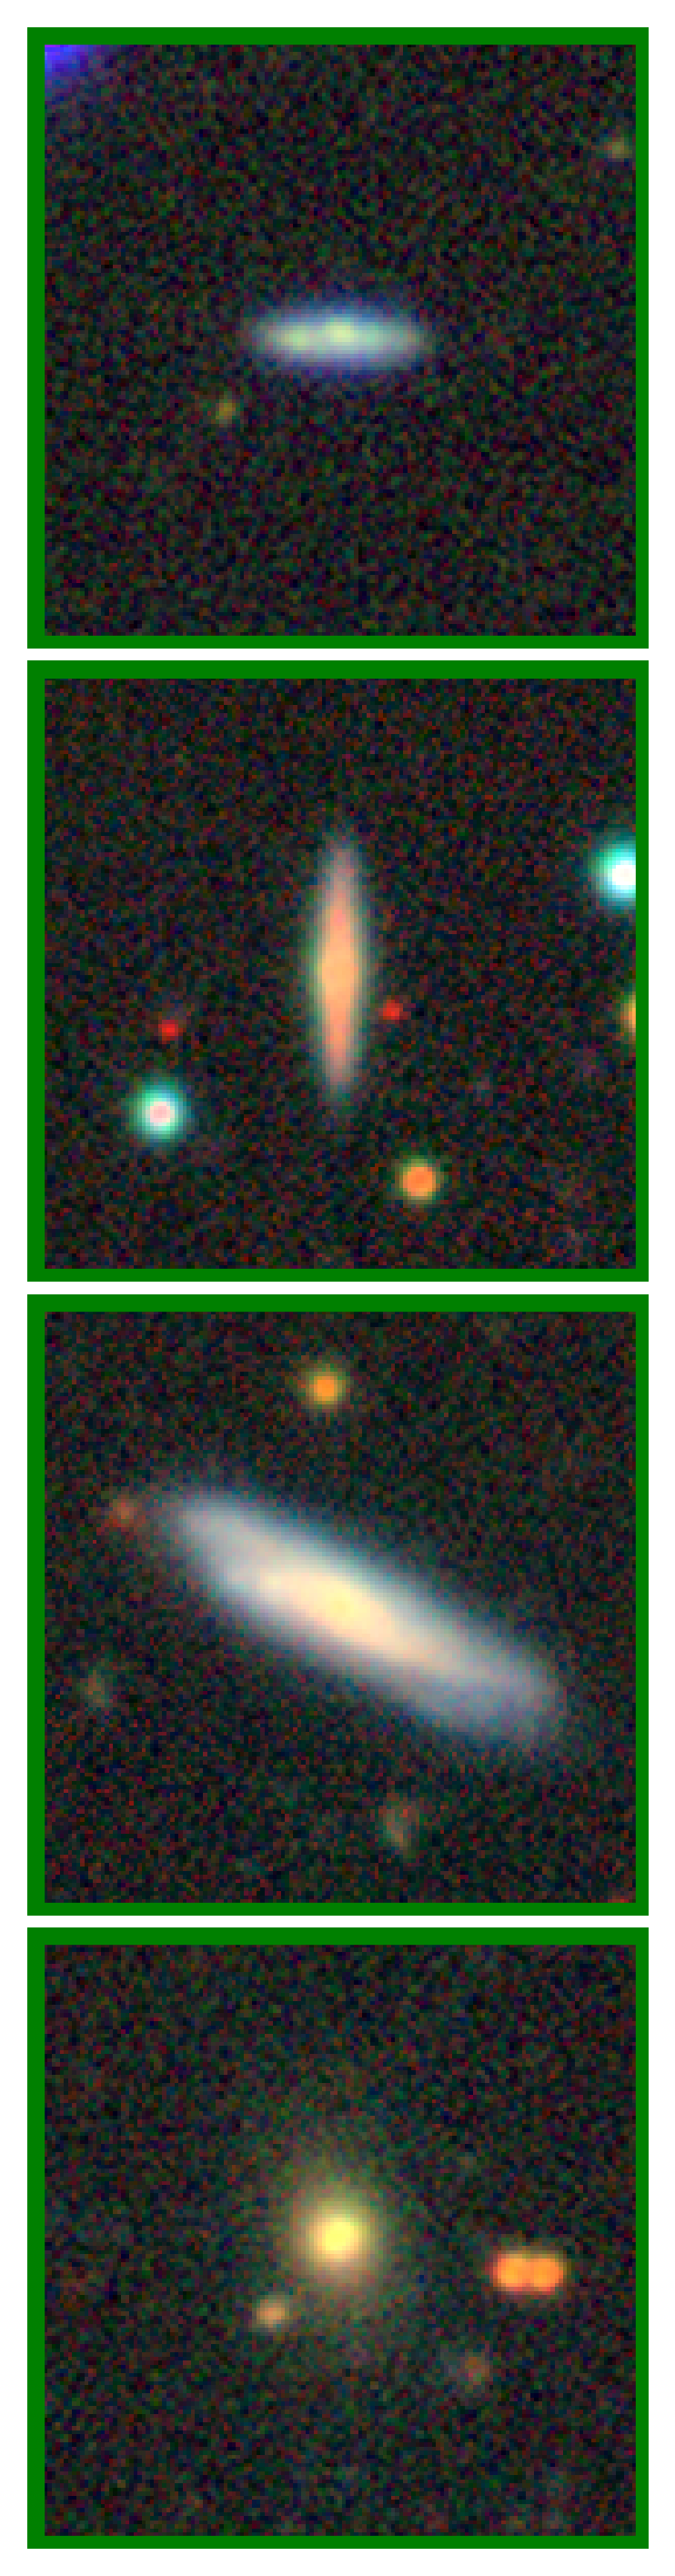
\includegraphics[height=0.21\textheight]{../figures/query_images.png}
        \caption{$\mathbf{z}_q$}
        \label{fig:retrieval_1}
    \end{subfigure}%
    \hfill
    \begin{subfigure}{0.22\textwidth}
        \centering
        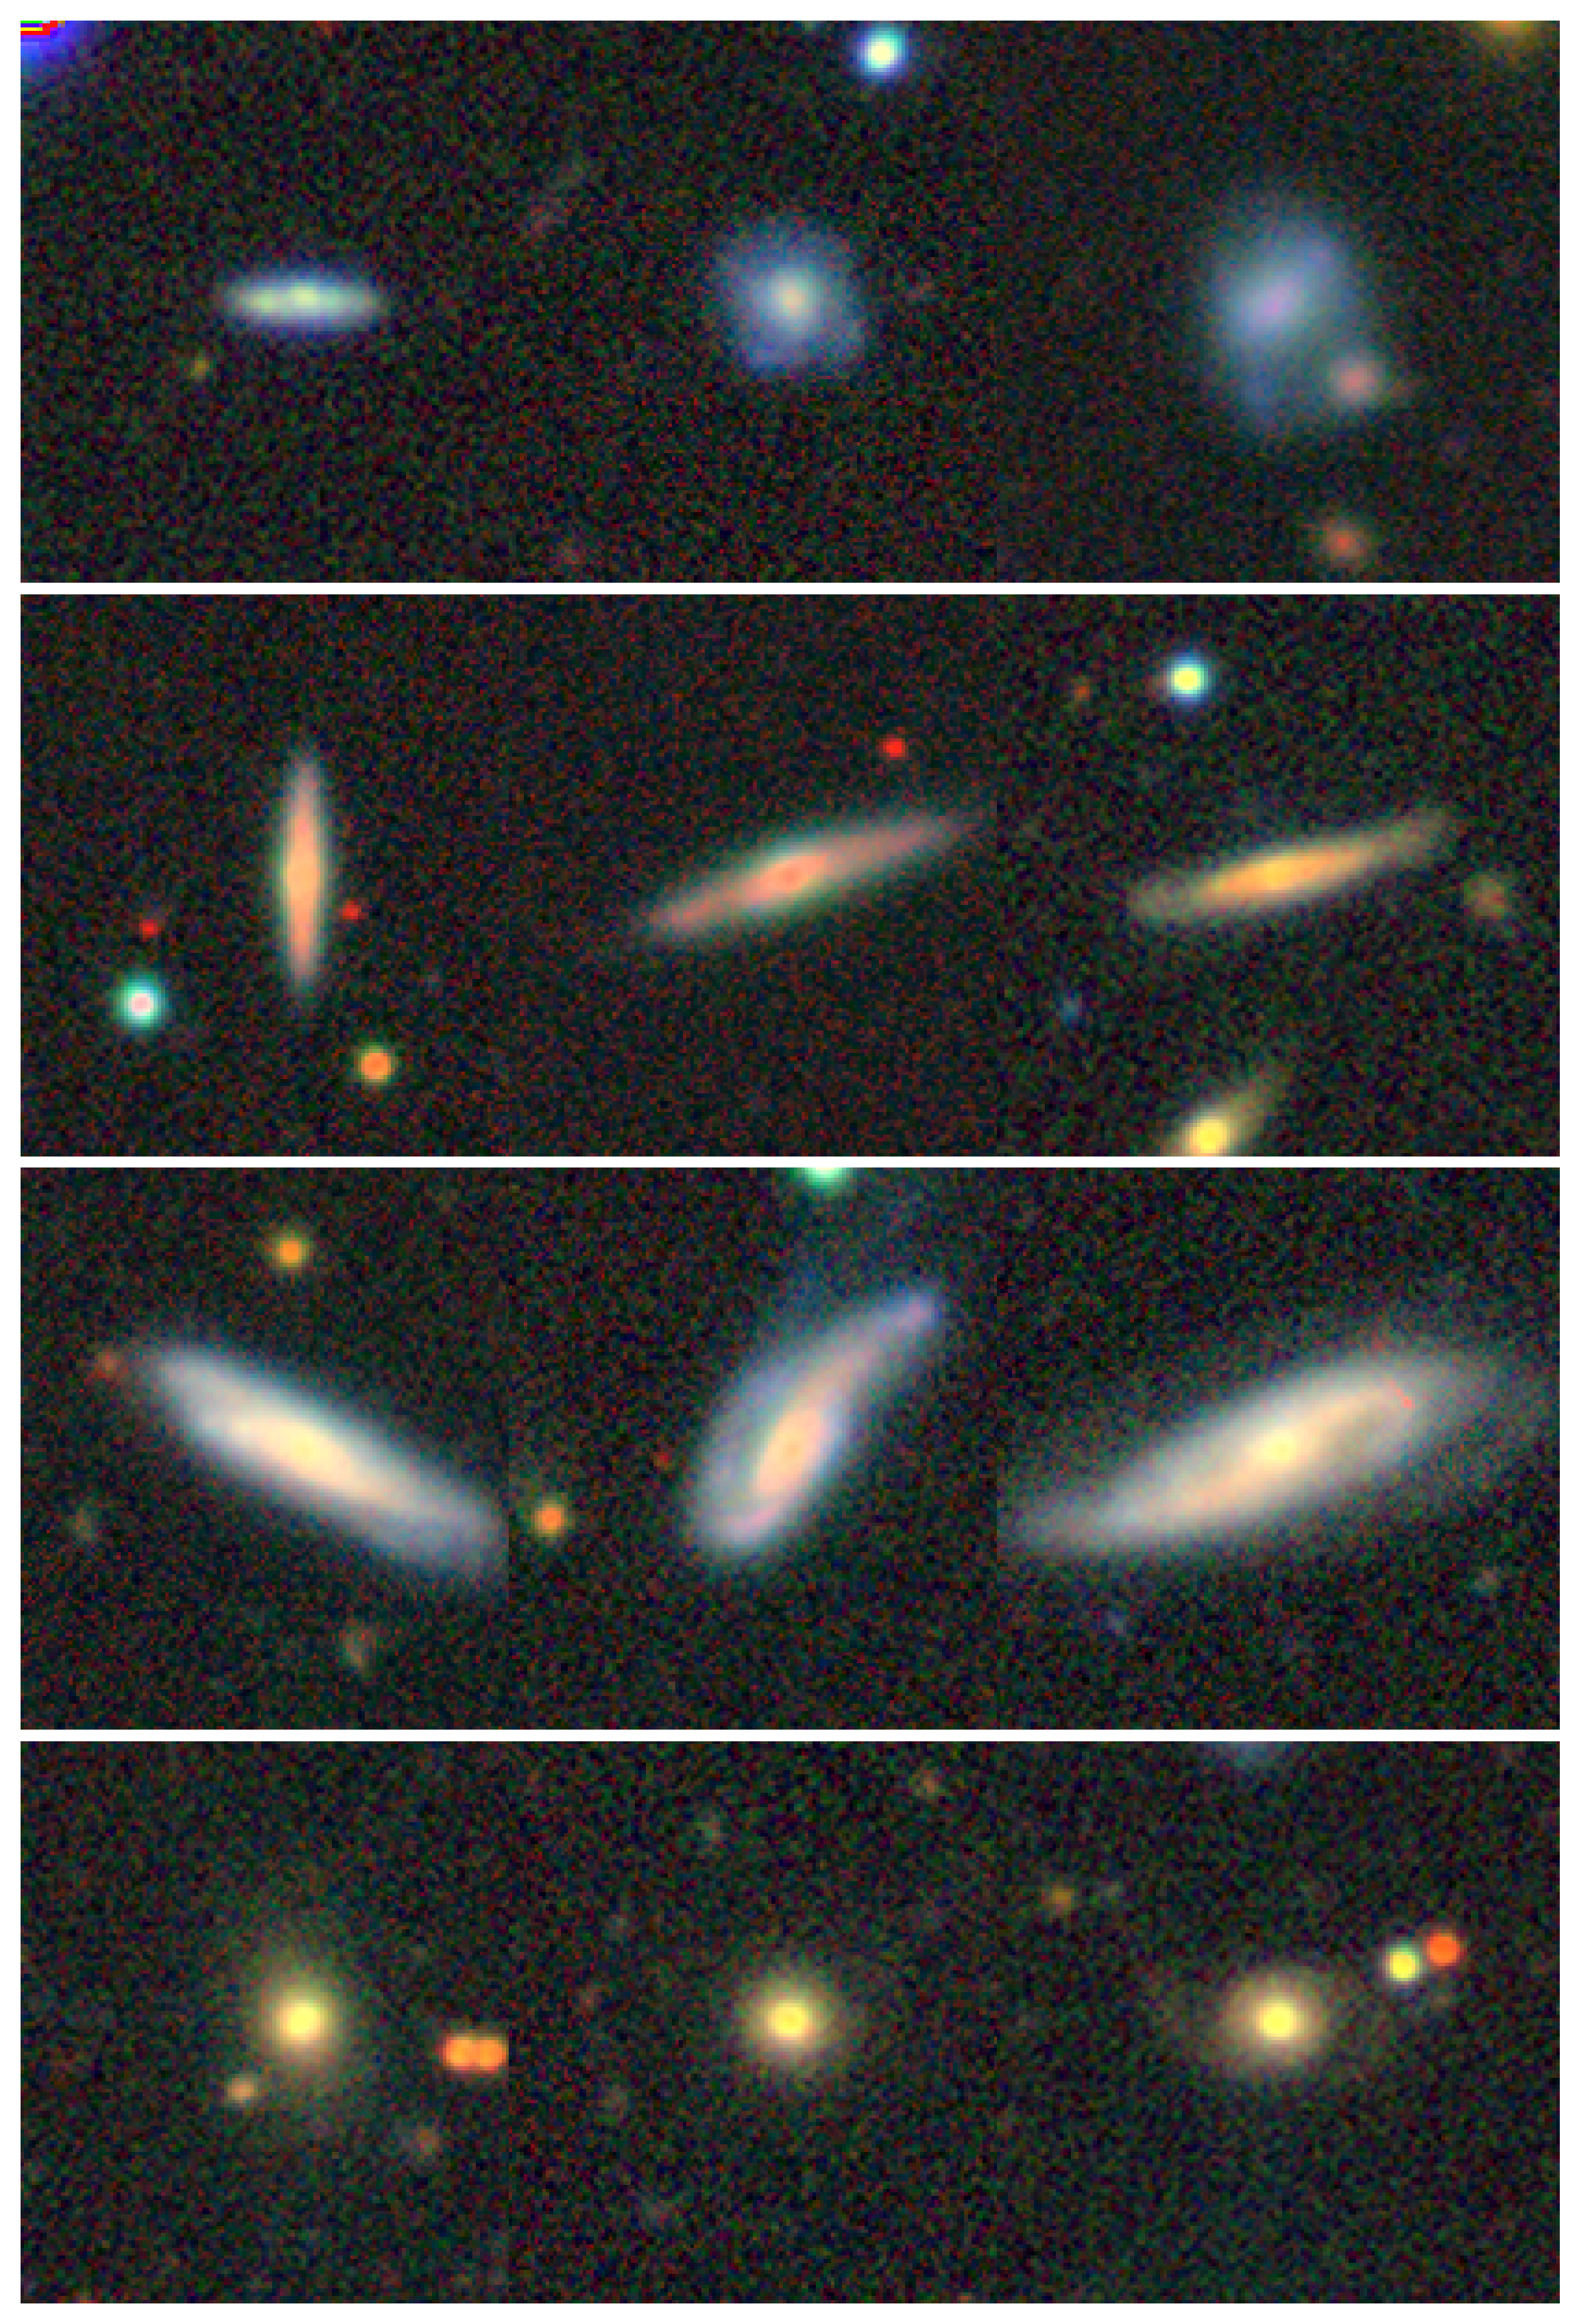
\includegraphics[height=0.21\textheight]{../figures/images_im_im.png}
        \caption{$S_C(\mathbf{z}_q^{im}, \mathbf{z}_j^{im})$}
        \label{fig:retrieval_2}
    \end{subfigure}%
    \hfill
    \begin{subfigure}{0.22\textwidth}
        \centering
        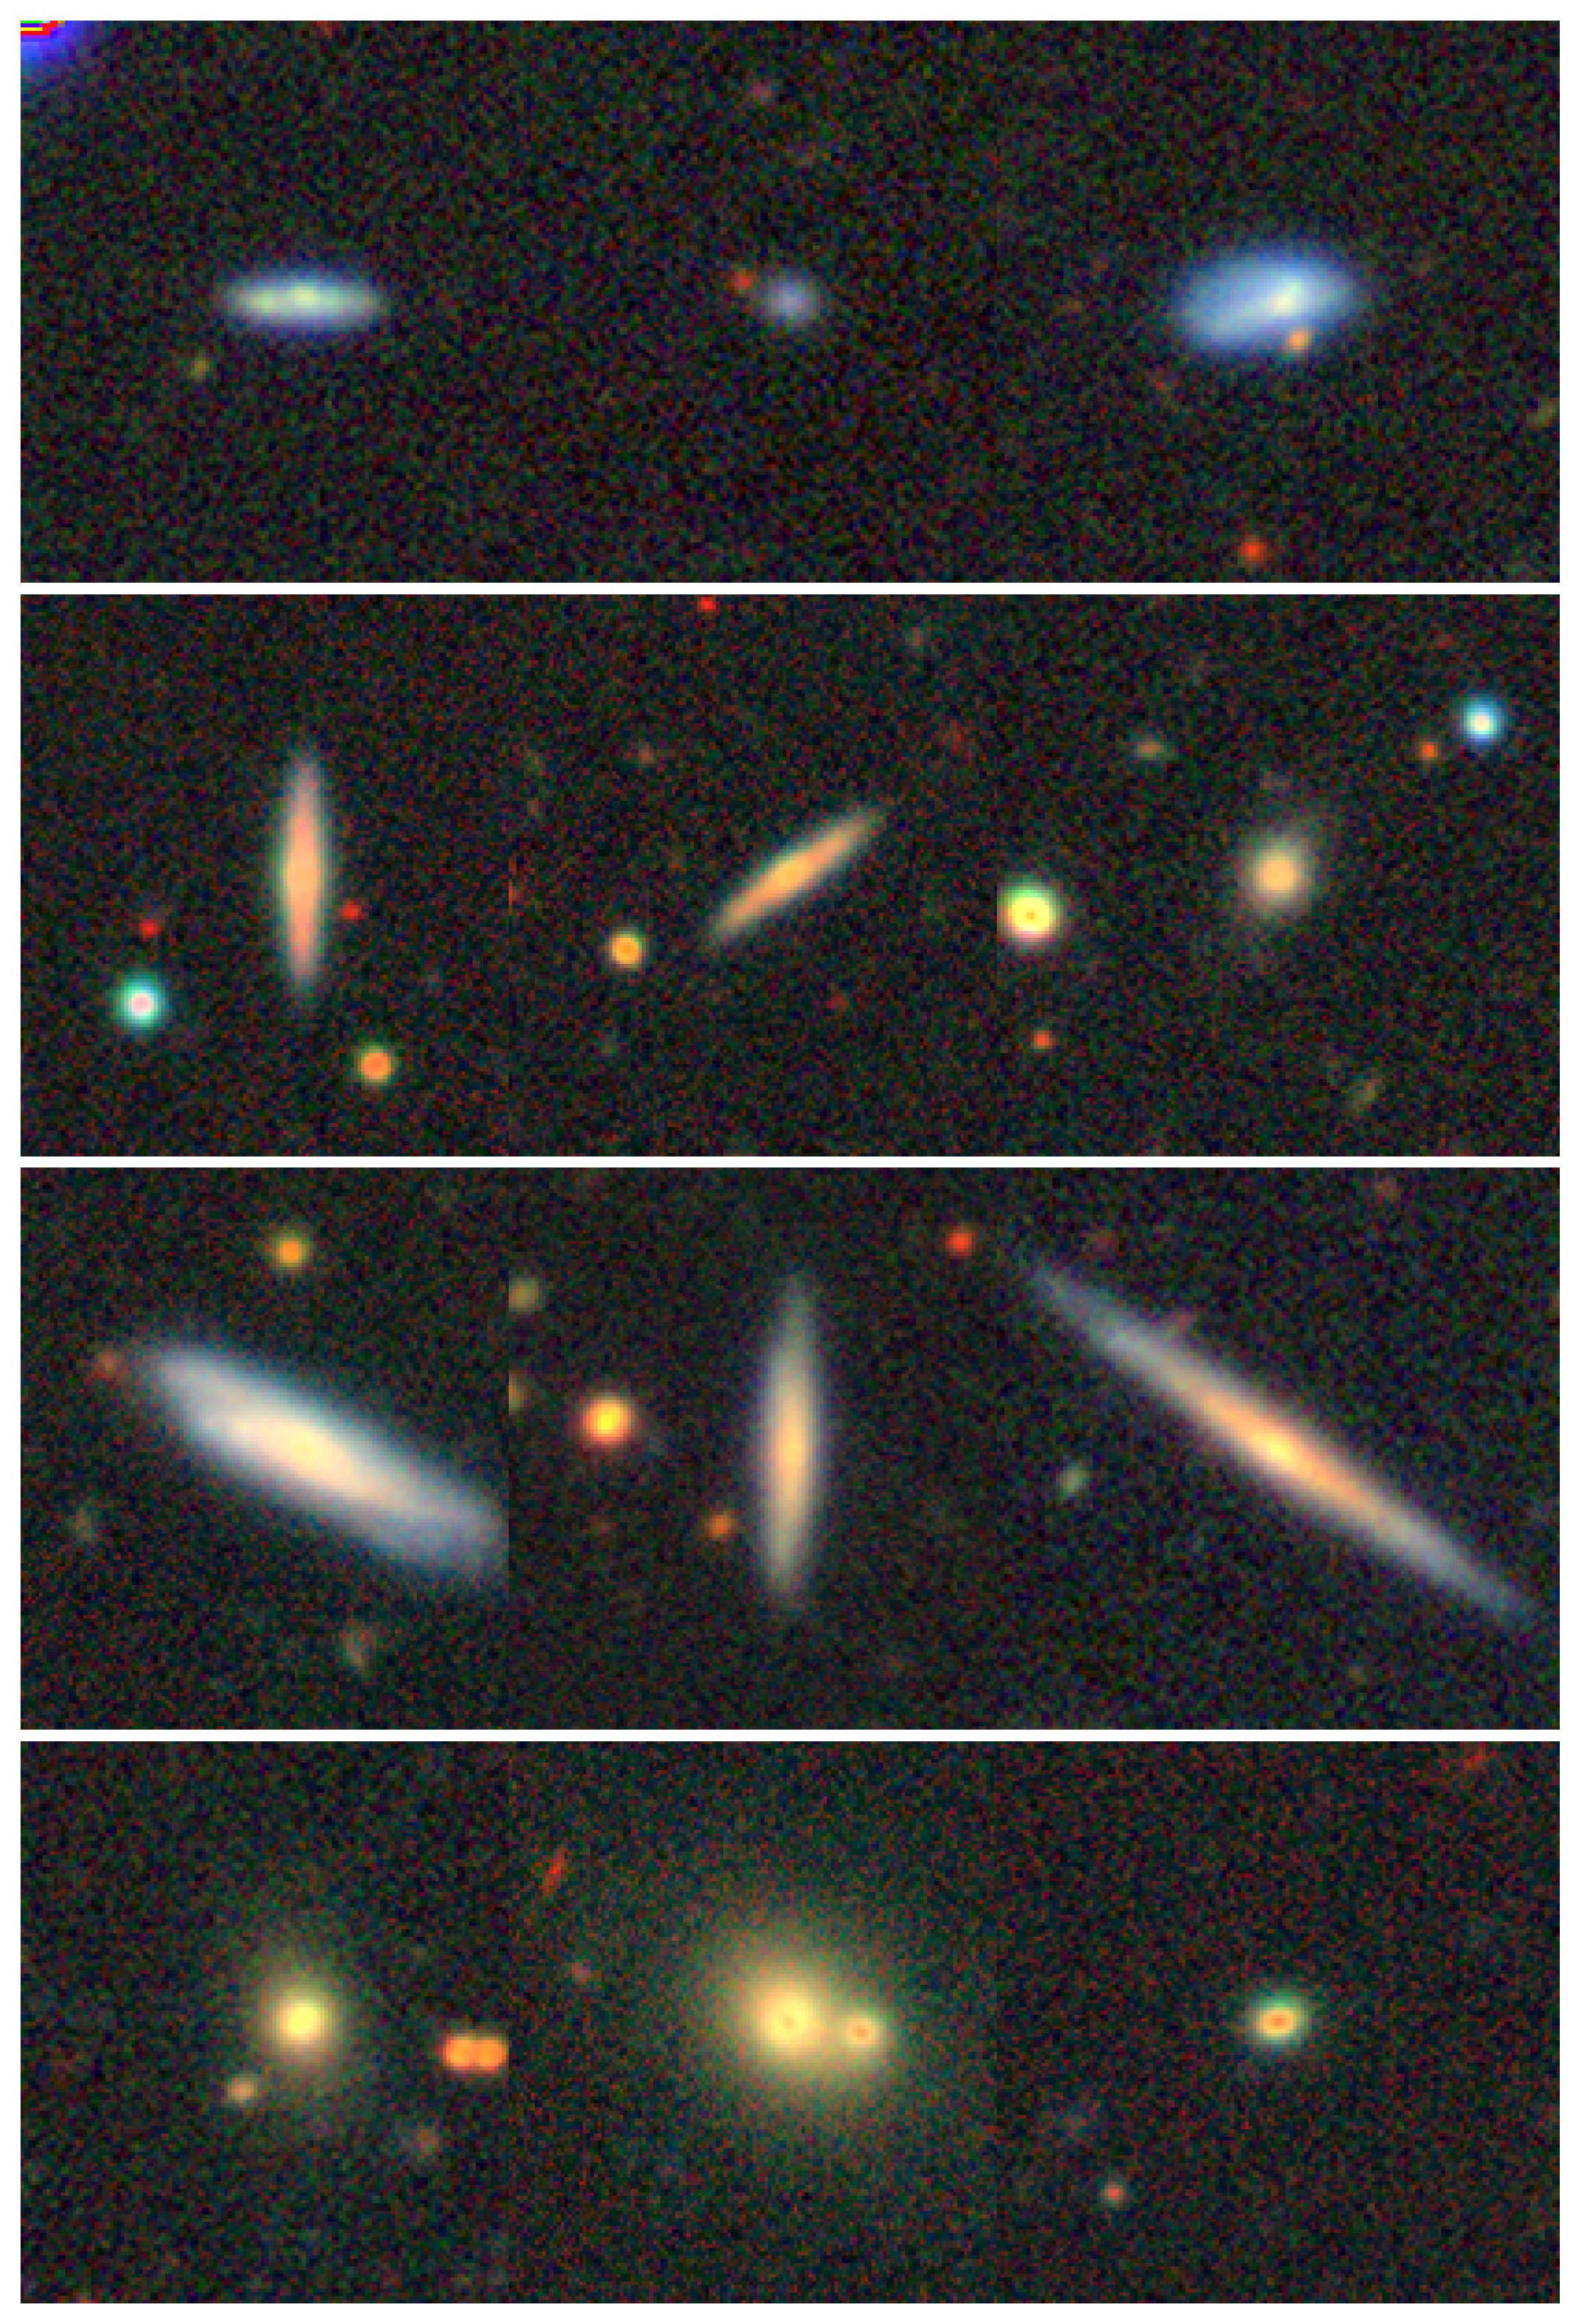
\includegraphics[height=0.21\textheight]{../figures/images_sp_sp.png}
        \caption{$S_C(\mathbf{z}_q^{sp}, \mathbf{z}_j^{sp})$}
        \label{fig:retrieval_3}
    \end{subfigure}%
    \hfill
    \begin{subfigure}{0.22\textwidth}
        \centering
        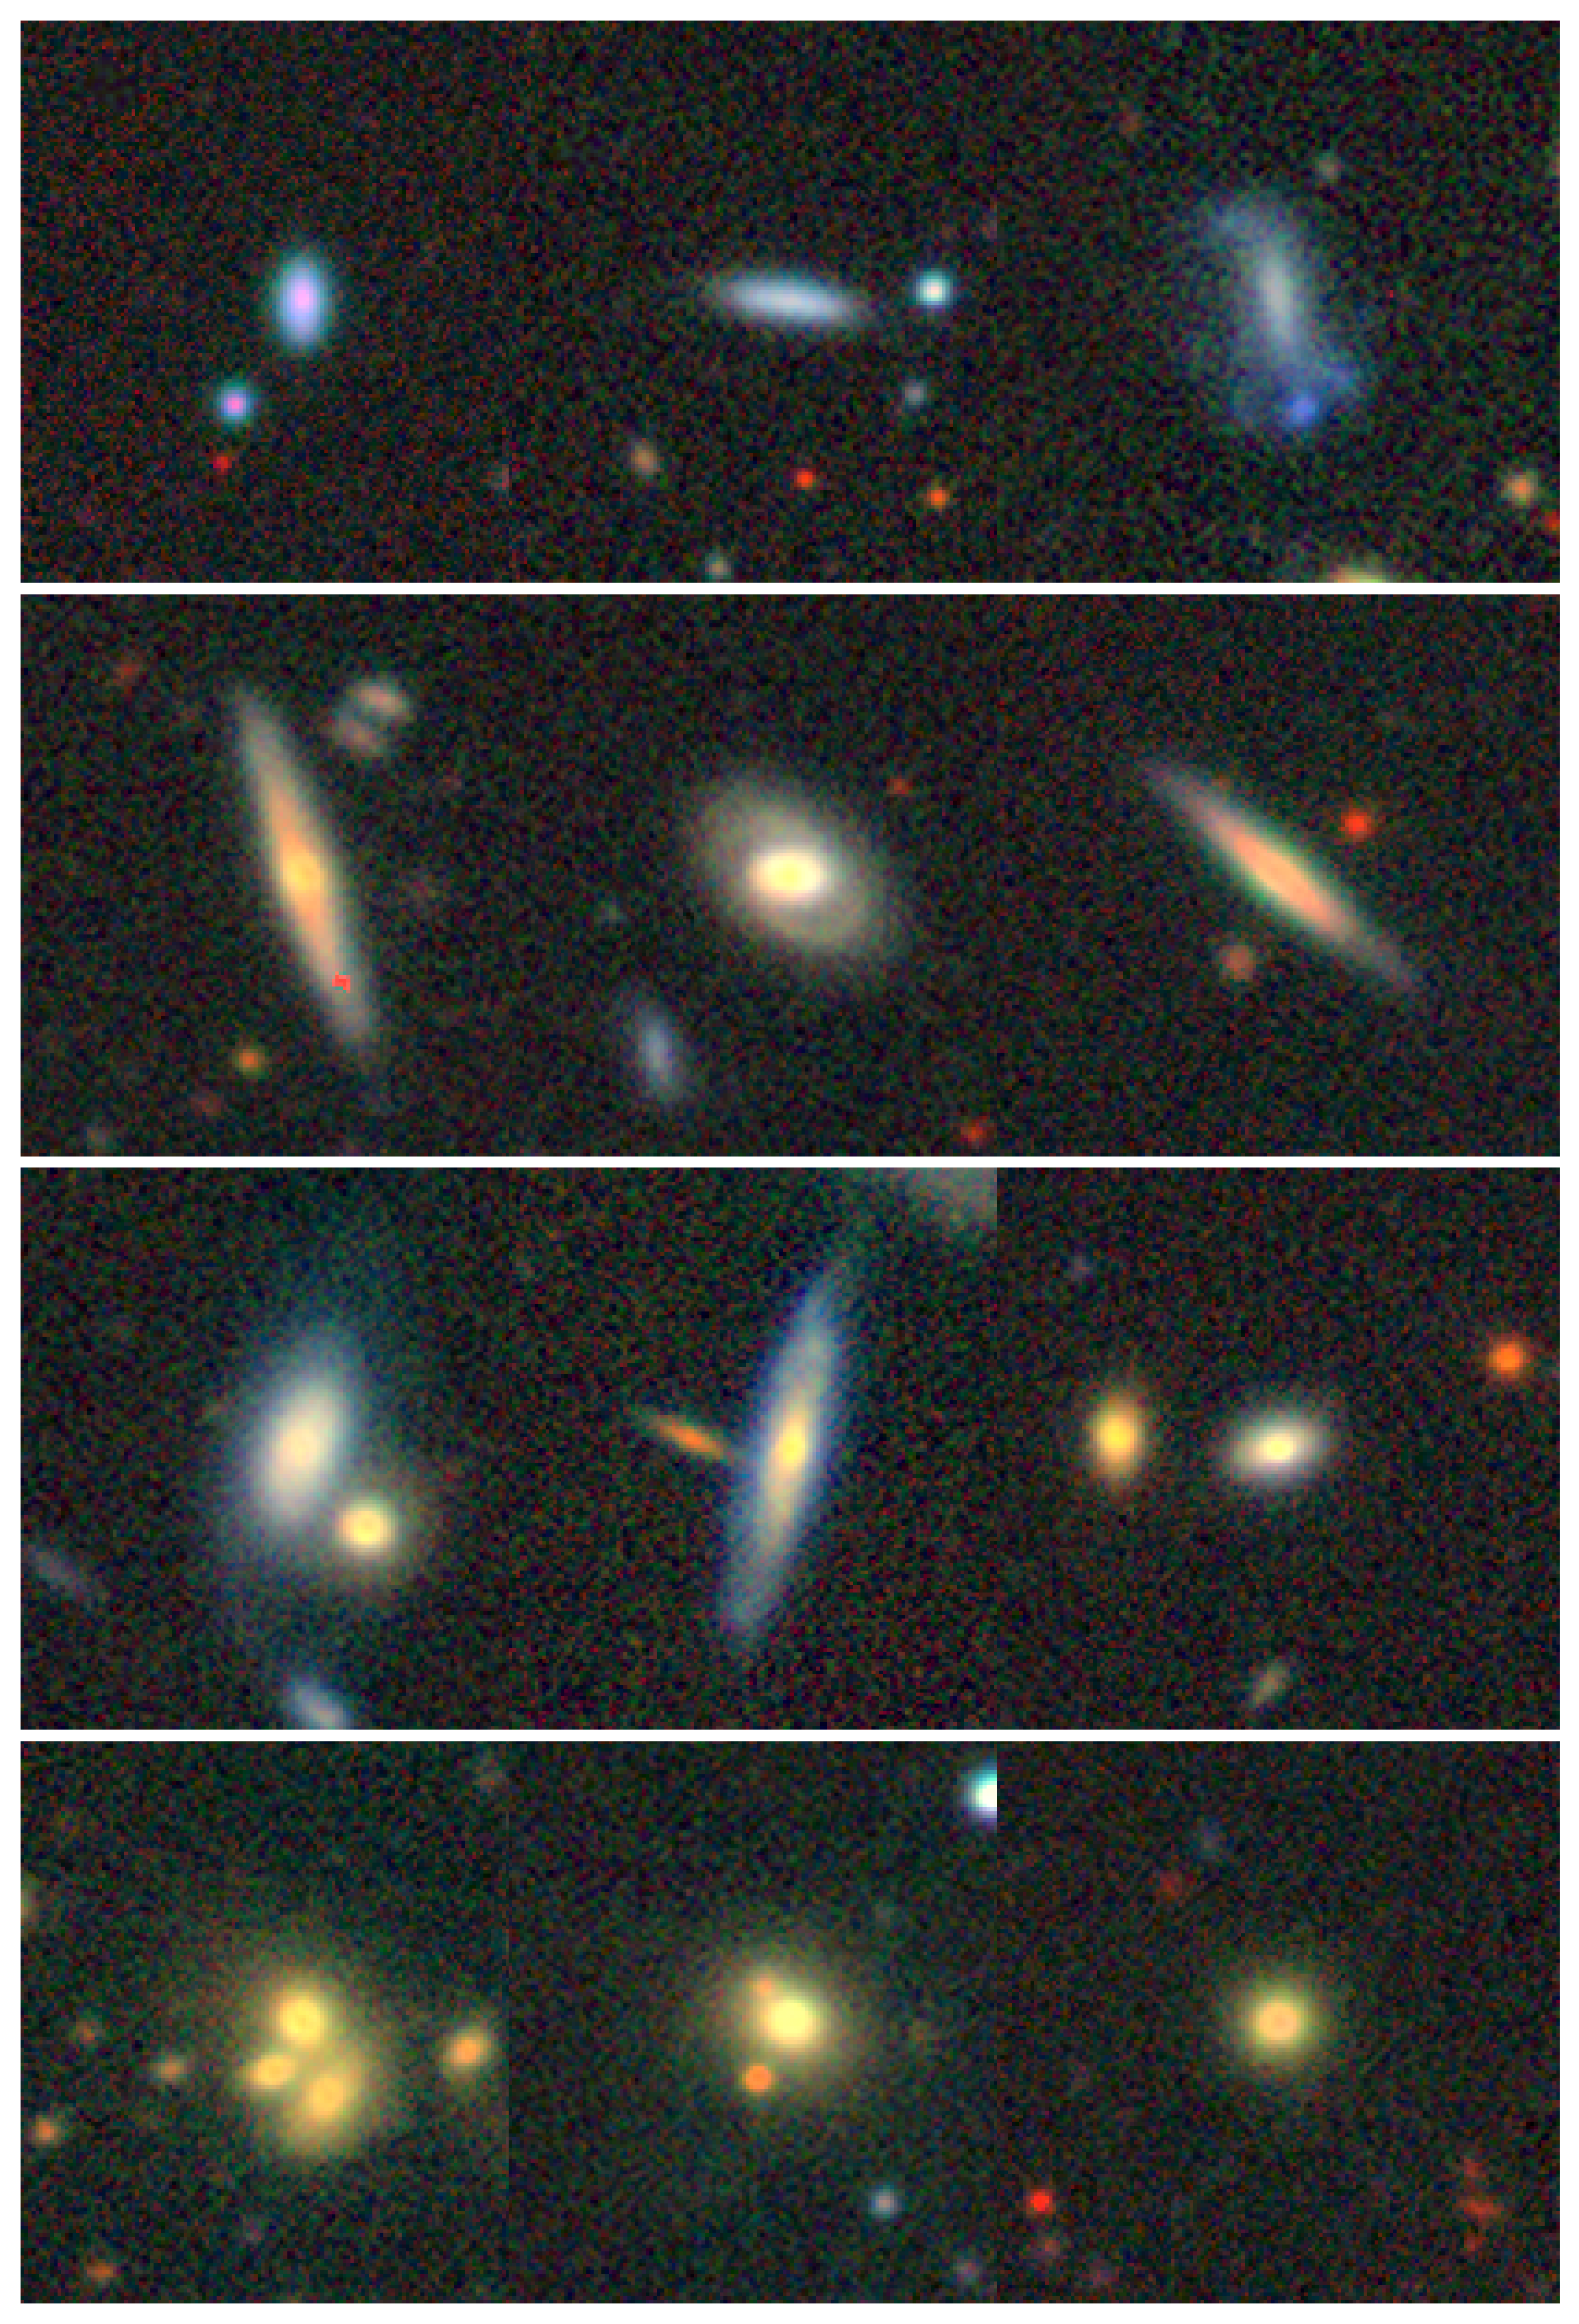
\includegraphics[height=0.21\textheight]{../figures/images_im_sp.png}
        \caption{$S_C(\mathbf{z}_q^{sp}, \mathbf{z}_j^{im})$}
        \label{fig:retrieval_4}
    \end{subfigure}%
    \hfill
    \begin{subfigure}{0.22\textwidth}
        \centering
        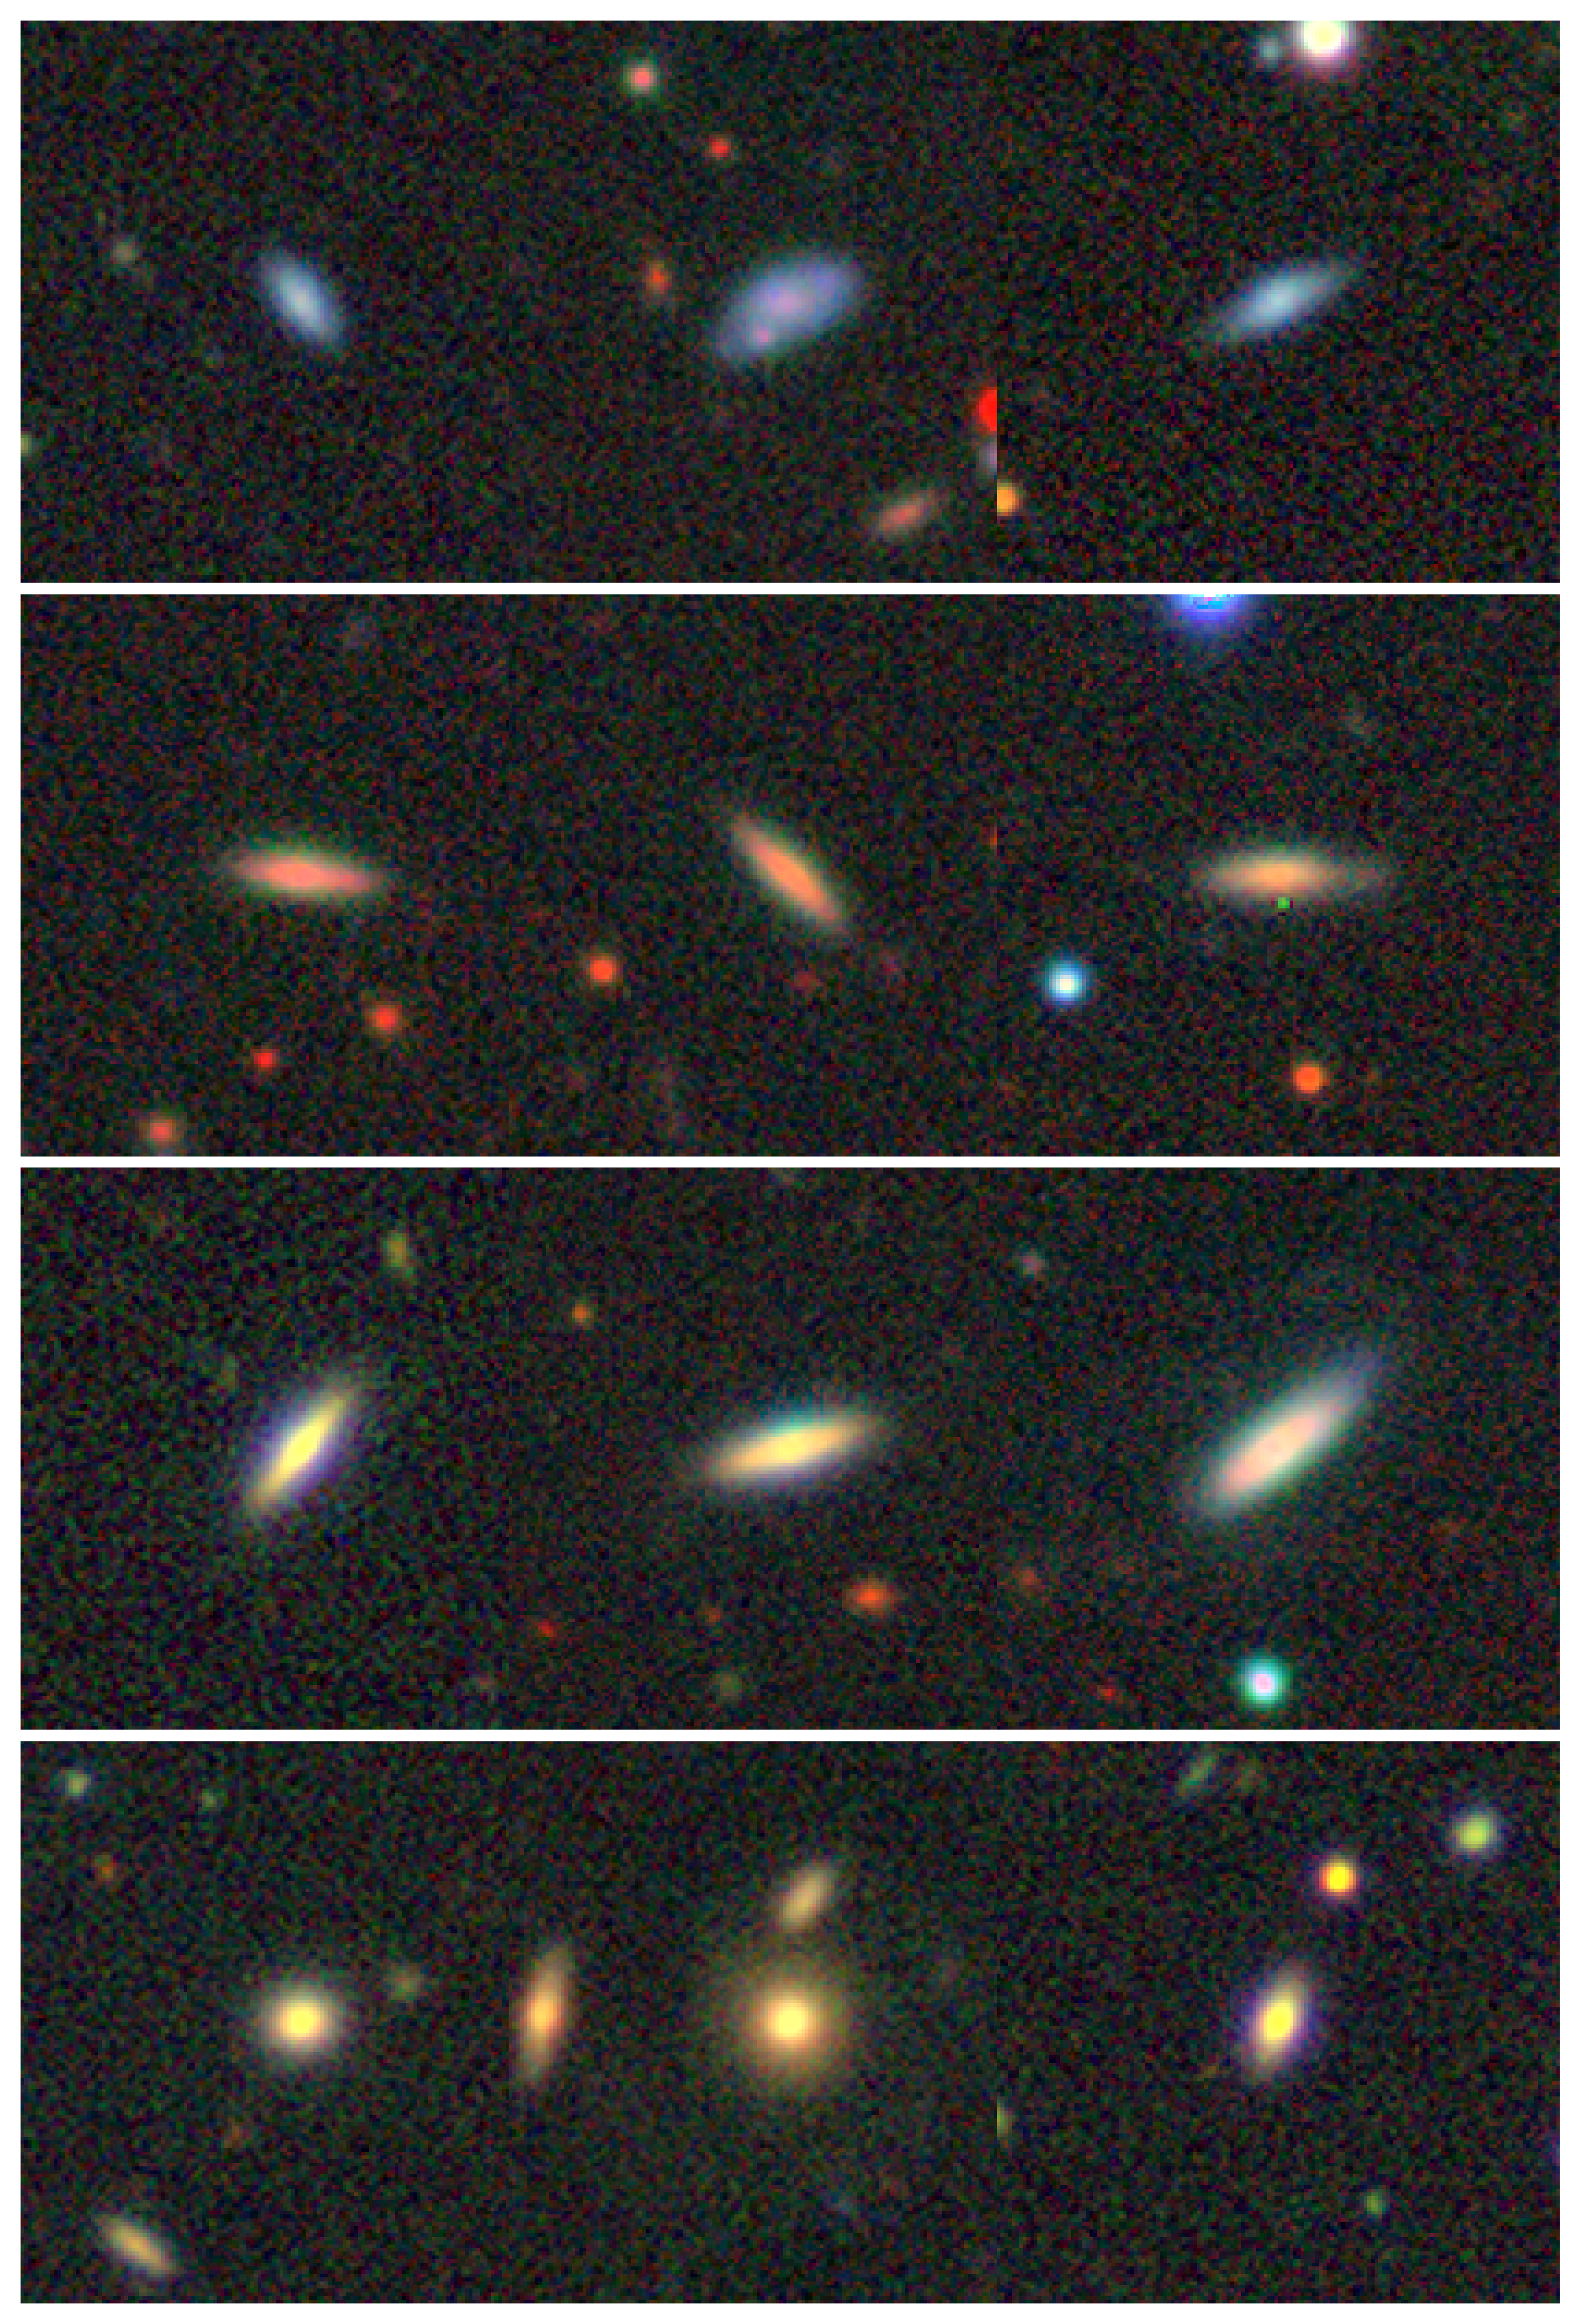
\includegraphics[height=0.21\textheight]{../figures/images_sp_im.png}
        \caption{$S_C(\mathbf{z}_q^{im}, \mathbf{z}_j^{sp})$}
        \label{fig:retrieval_5}
    \end{subfigure}
    \caption{Your overall figure caption here.}
    \label{fig:retrieval}
\end{figure}
We further illustrate the search capabilities of this model by presenting the retrieved spectra for some of the randmly chosen query galaxies for all four possible combinations of modalities in Fig.\ref{fig:spectral_retrieval}. The 5 most similar spectra are shown for each query galaxy. The model is largely able to retrieve spectra similar to the query galaxy, in all modality pair combinations. This is both in terms of the overall shape of the spectrum and the presence of specific spectral features, such as particular spikes. This further demonstrates the model's ability to align the image and spectrum embeddings in the shared latent space.

This search abilit can be useful in a variety of applications, such as seach for rare or unusual objects (see some examples of this in Ref.\cite{stein}). The results are largely consistent with the original work, although a direct comparison is difficult as the images and spectra chosen for queries are random. It is worth noting that our results are achieved using a much smaller model the original work, but yields (visually) similar results.

\begin{figure}[H]
    \centering
    % First row
    \begin{subfigure}[b]{0.45\textwidth}
        \centering
        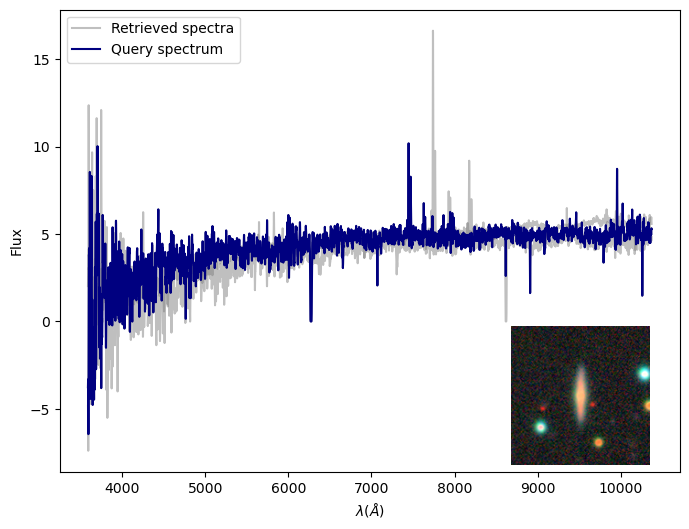
\includegraphics[width=\textwidth]{../figures/spectral_retrieval_im_im_1}
        \caption{$S_C(\mathbf{z}_q^{im}, \mathbf{z}_j^{im})$}
        \label{fig:im_im_1}
    \end{subfigure}%
    \hfill
    \begin{subfigure}[b]{0.45\textwidth}
        \centering
        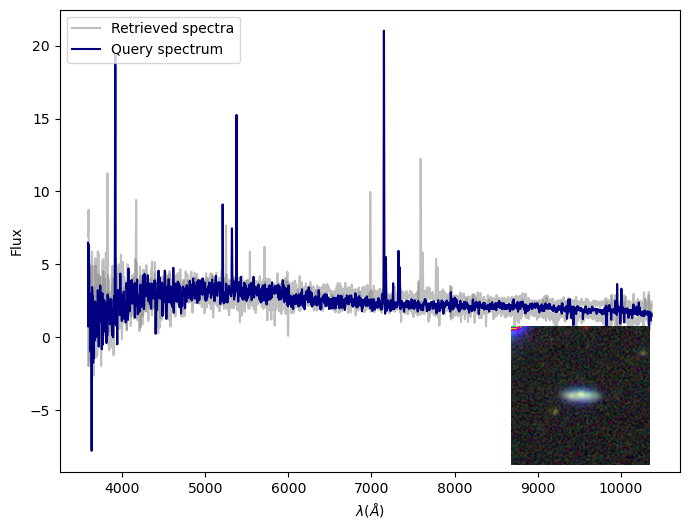
\includegraphics[width=\textwidth]{../figures/spectral_retrieval_im_im_2}
        \caption{$S_C(\mathbf{z}_q^{im}, \mathbf{z}_j^{im})$}
        \label{fig:im_im_2}
    \end{subfigure}

    % Second row
    \begin{subfigure}[b]{0.45\textwidth}
        \centering
        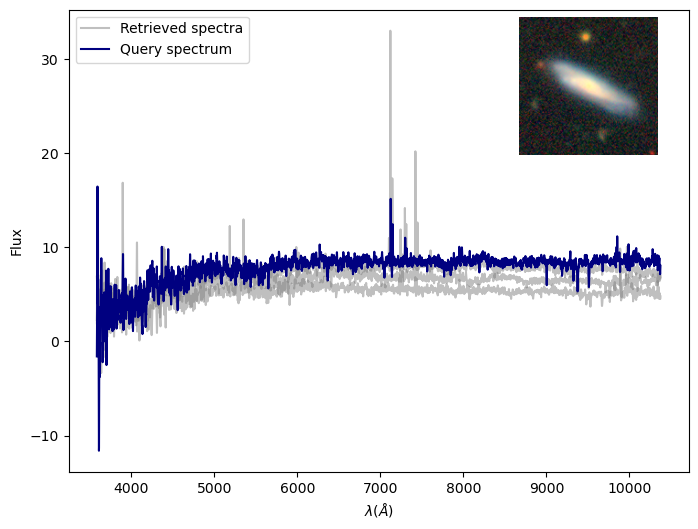
\includegraphics[width=\textwidth]{../figures/spectral_retrieval_im_sp_1}
        \caption{$S_C(\mathbf{z}_q^{sp}, \mathbf{z}_j^{im})$}
        \label{fig:im_sp_1}
    \end{subfigure}%
    \hfill
    \begin{subfigure}[b]{0.45\textwidth}
        \centering
        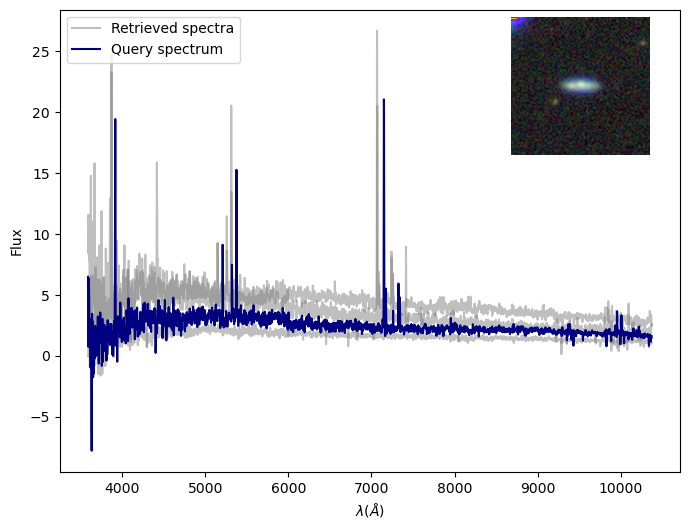
\includegraphics[width=\textwidth]{../figures/spectral_retrieval_im_sp_2}
        \caption{$S_C(\mathbf{z}_q^{sp}, \mathbf{z}_j^{im})$}
        \label{fig:im_sp_2}
    \end{subfigure}

    % Third row
    \begin{subfigure}[b]{0.45\textwidth}
        \centering
        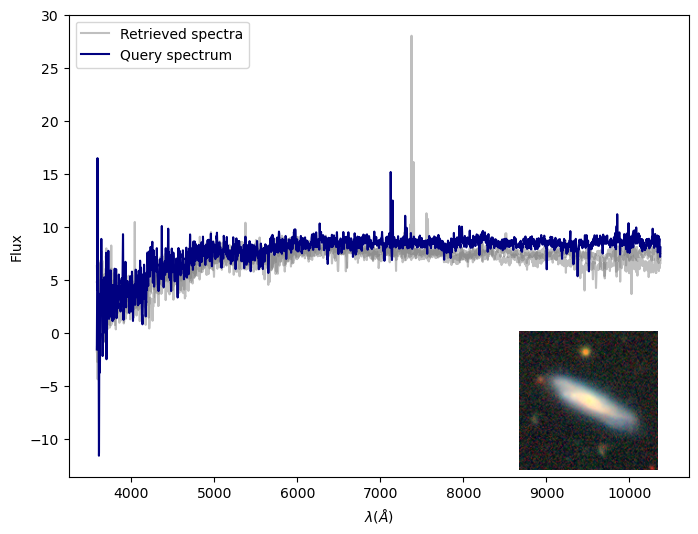
\includegraphics[width=\textwidth]{../figures/spectral_retrieval_sp_im_1}
        \caption{$S_C(\mathbf{z}_q^{im}, \mathbf{z}_j^{sp})$}
        \label{fig:sp_im_1}
    \end{subfigure}%
    \hfill
    \begin{subfigure}[b]{0.45\textwidth}
        \centering
        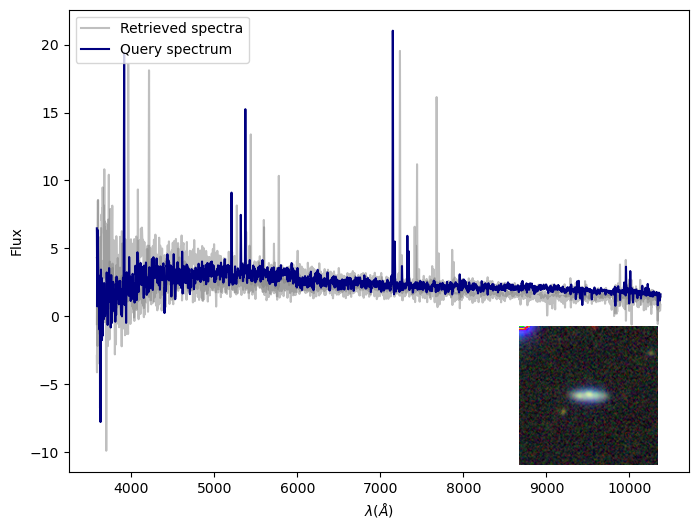
\includegraphics[width=\textwidth]{../figures/spectral_retrieval_sp_im_2}
        \caption{$S_C(\mathbf{z}_q^{im}, \mathbf{z}_j^{sp})$}
        \label{fig:sp_im_2}
    \end{subfigure}

    % Fourth row
    \begin{subfigure}[b]{0.45\textwidth}
        \centering
        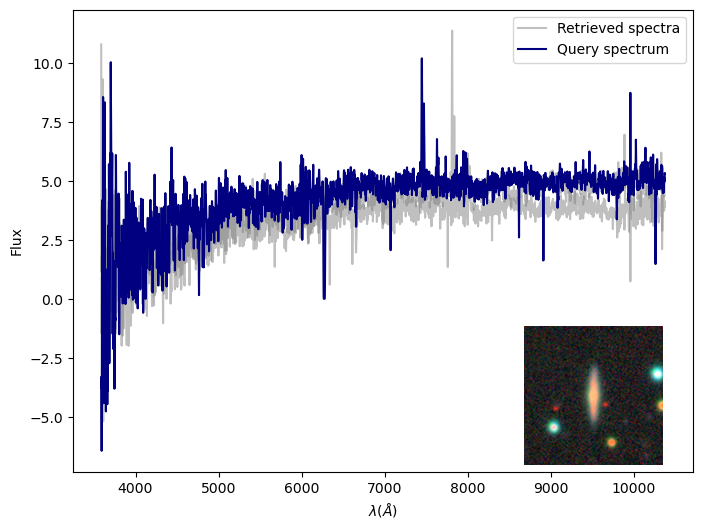
\includegraphics[width=\textwidth]{../figures/spectral_retrieval_sp_sp_1}
        \caption{$S_C(\mathbf{z}_q^{sp}, \mathbf{z}_j^{sp})$}
        \label{fig:sp_sp_1}
    \end{subfigure}%
    \hfill
    \begin{subfigure}[b]{0.45\textwidth}
        \centering
        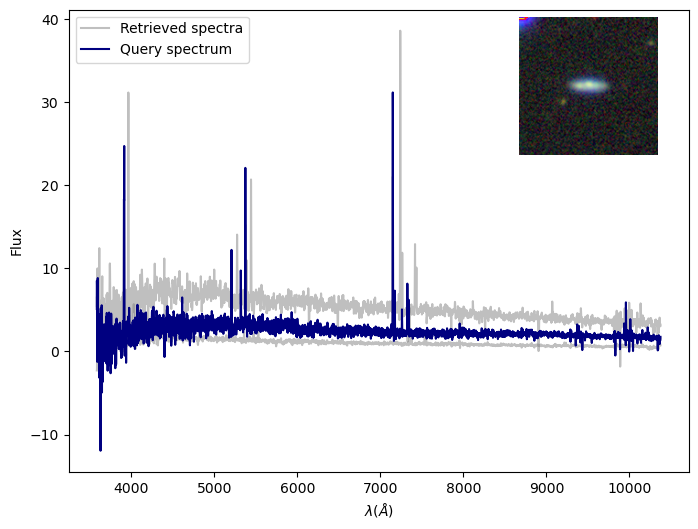
\includegraphics[width=\textwidth]{../figures/spectral_retrieval_sp_sp_2}
        \caption{$S_C(\mathbf{z}_q^{sp}, \mathbf{z}_j^{sp})$}
        \label{fig:sp_sp_2}
    \end{subfigure}

    \caption{Spectral retrieval for random query galaxies in the validation set. The top 5 most similar spectra are shown for each query galaxy, pictured in each graph. This was done using image-image search for (\ref{fig:im_im_1}) (\ref{fig:im_im_2}), image-spectrum search for (\ref{fig:im_sp_1}) (\ref{fig:im_sp_2}), spectrum-image search for (\ref{fig:sp_im_1}) (\ref{fig:sp_im_2}) and spectrum-spectrum search for (\ref{fig:sp_sp_1}) (\ref{fig:sp_sp_2}).}
    \label{fig:spectral_retrieval}
\end{figure}


\subsection{Zero Shot Prediction of Physical Properties}
We present the results of the zero-shot prediction of redshift and stellar mass in Fig.\ref{fig:zeroshot}. These plots depict a scatterplot of the $k$-NN with 16 neighbours predictions against the ProvaBGS catalogue values for the validation set (grey points). A 2-D histogram ise also plotted with a heatmap help visualise the joint distribution of the two variables. Additionally, a Kerndel Density Estimate (KDE) plot is used to overlay cotnour lines (in black) that represent levels of density over the scatter plot. The coefficient of determination $R^2$ score is also calculated for each prediction, which is a measure on the proportion of variance that is explained by the model.

The $k$-NN regression is performed for both in-modality and cross-modality regression; for in-modality, we refer to case of using the same modality embeddings (image embeddings or spectrum embeddings) for both trainign and predicting the physical properties, while for cross-modality, we refer to the case of using spectrum embeddings for training and image embeddings for predicting. 

We can conclude that, similar to the original work, our embeddings give a strong zero-shot performance, indicating that the embedding space is able to organise itself around physically meaningful properties. The significanlty good performance even in the cross-modal case indicates that the neigbous in our embedded space indeed share physically meaningful features. Similar to the original work, the in-modality regression outperforms the cross-modality regression, which showcases that despite training under the objective of bringing the two modalities together, this causes the emergent property of sharing information across modalities, as it helps structure the embedding space within each modality. Even though redshift was not an information explicitly used in the training, the spectrum-spectrum regression for redshift is able to capture a very high 0.87 of the variance in the data. This means that redshift was used as a naturally emergent property which aided the spectrum encoder to structure the embedding space.

Our reproduction results are consistent with the original work, but we note that we slightly underperform in all cases. This could be due to the smaller spectrum model used in our work. It could also be due to the model arhitecture itself, as the original work uses a transformer-based model which could capture a more nuanced representation of the spectra. Table \ref{tab:zeroshot} compares our results to the original work.


% Please add the following required packages to your document preamble:
% \usepackage{multirow}
\begin{table}[H]
    \begin{tabular}{clcc}
    \hline
    \textbf{Physical Property}    &                     & \begin{tabular}[c]{@{}c@{}}Original Work\\ $R^2$\end{tabular} & \begin{tabular}[c]{@{}c@{}}Our Reproduction\\ $R^2$\end{tabular} \\ \hline
    \hline
    \multirow{3}{*}{Redshift}     & Image Embeddings    & 0.71                                                          & 0.65                                                             \\
                                  & Spectrum Embeddings & 0.97                                                          & 0.87                                                             \\
                                  & Cross-Modal         & 0.64                                                          & 0.59                                                             \\ \hline
    \multirow{3}{*}{Stellar Mass} & Image Embeddings    & 0.66                                                          & 0.57                                                             \\
                                  & Spectrum Embeddings & 0.86                                                          & 0.74                                                             \\
                                  & Cross-Modal         & 0.58                                                          & 0.50                                                             \\ \hline
    \end{tabular}
    \caption{Comparison of $R^2$ scores for zero-shot prediction of redshift and stellar mass between the original AstroCLIP paper and our reproduction. By Cross-modal, we refer to the case of using spectrum embeddings for training of $k$-NN regression and image embeddings for prediction. For in-modality, we refer to the case of using the same modality embeddings for both training and prediction.}
    \label{tab:zeroshot}
\end{table}





\begin{figure}[H]
    \centering
    % Row 1: Image Embeddings
    \begin{subfigure}[b]{0.48\textwidth}
        \centering
        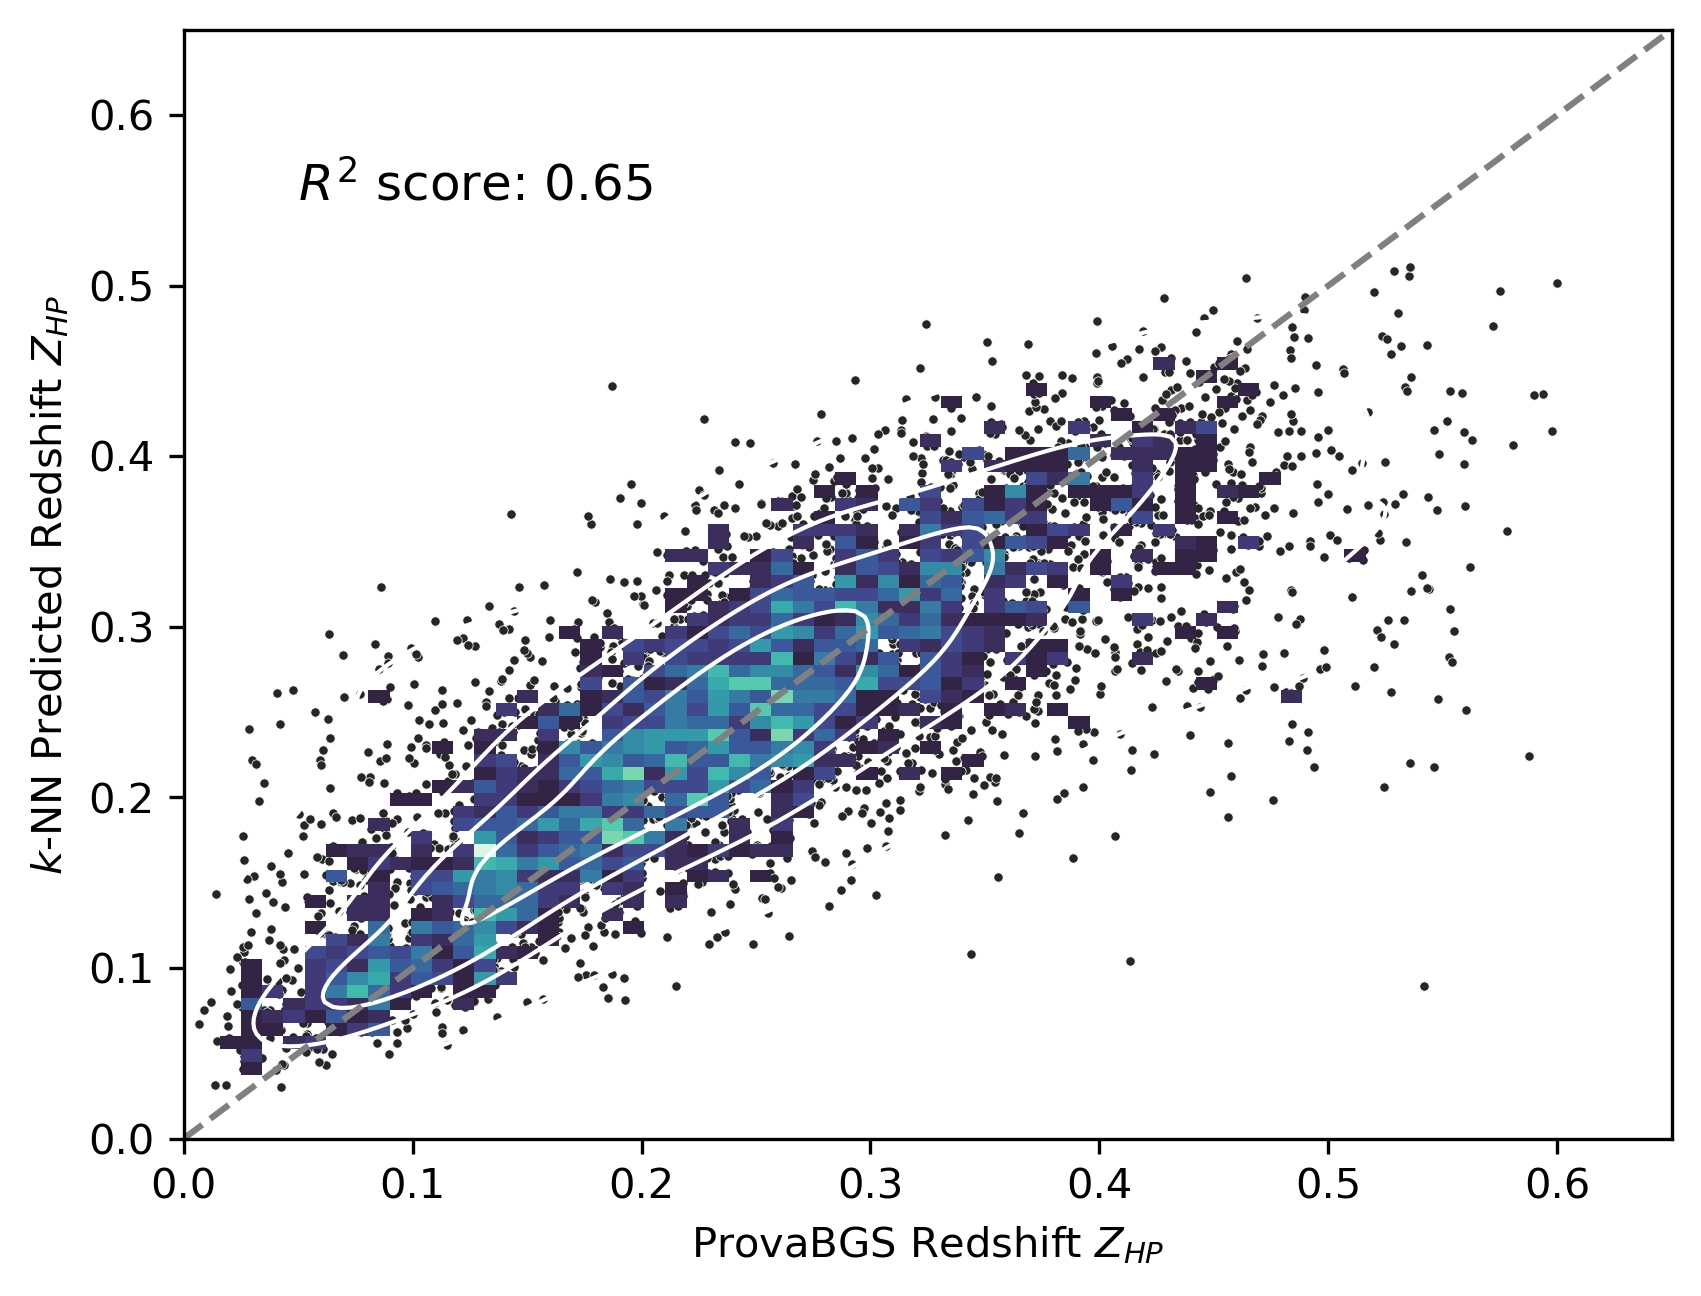
\includegraphics[width=\textwidth]{../figures/zeroshot_redshift_image.png}
        \caption{Image Embeddings for Redshift}
        \label{fig:redshift_image}
    \end{subfigure}%
    \hfill
    \begin{subfigure}[b]{0.48\textwidth}
        \centering
        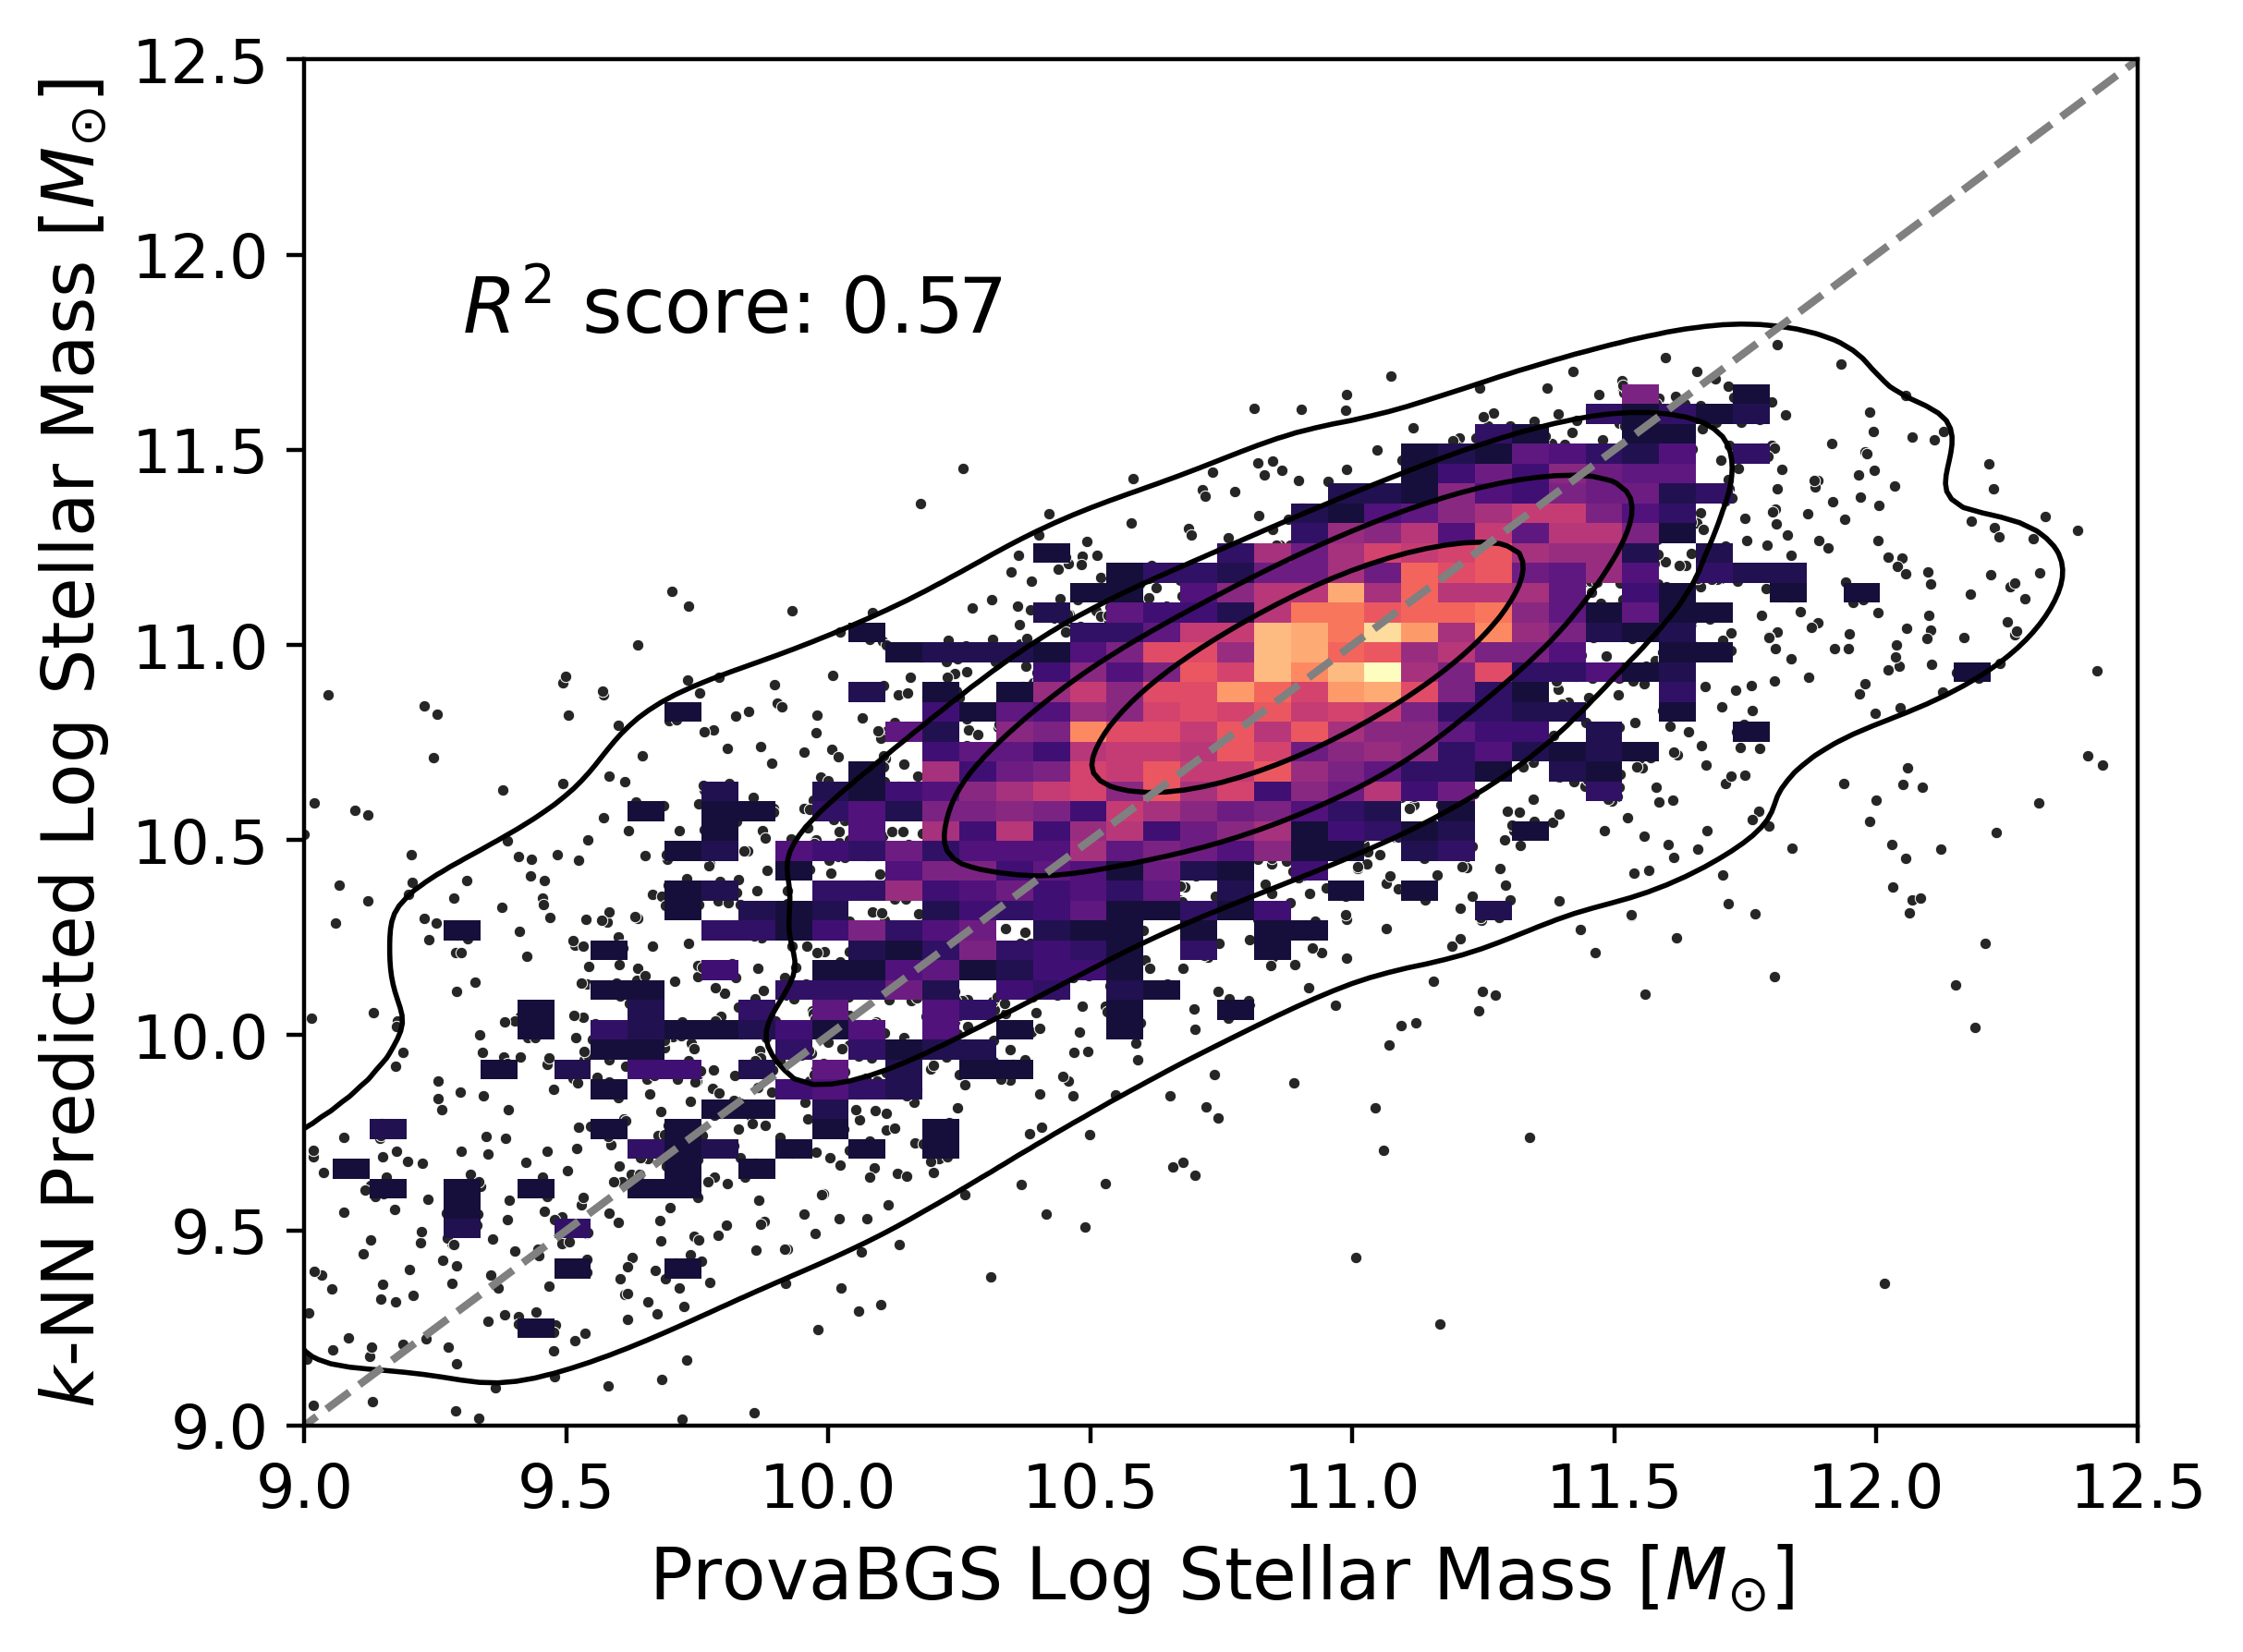
\includegraphics[width=\textwidth]{../figures/zeroshot_stellarmass_image.png}
        \caption{Image Embeddings for Stellar Mass}
        \label{fig:stellarmass_image}
    \end{subfigure}
    
    % Row 2: Spectrum Embeddings
    \begin{subfigure}[b]{0.48\textwidth}
        \centering
        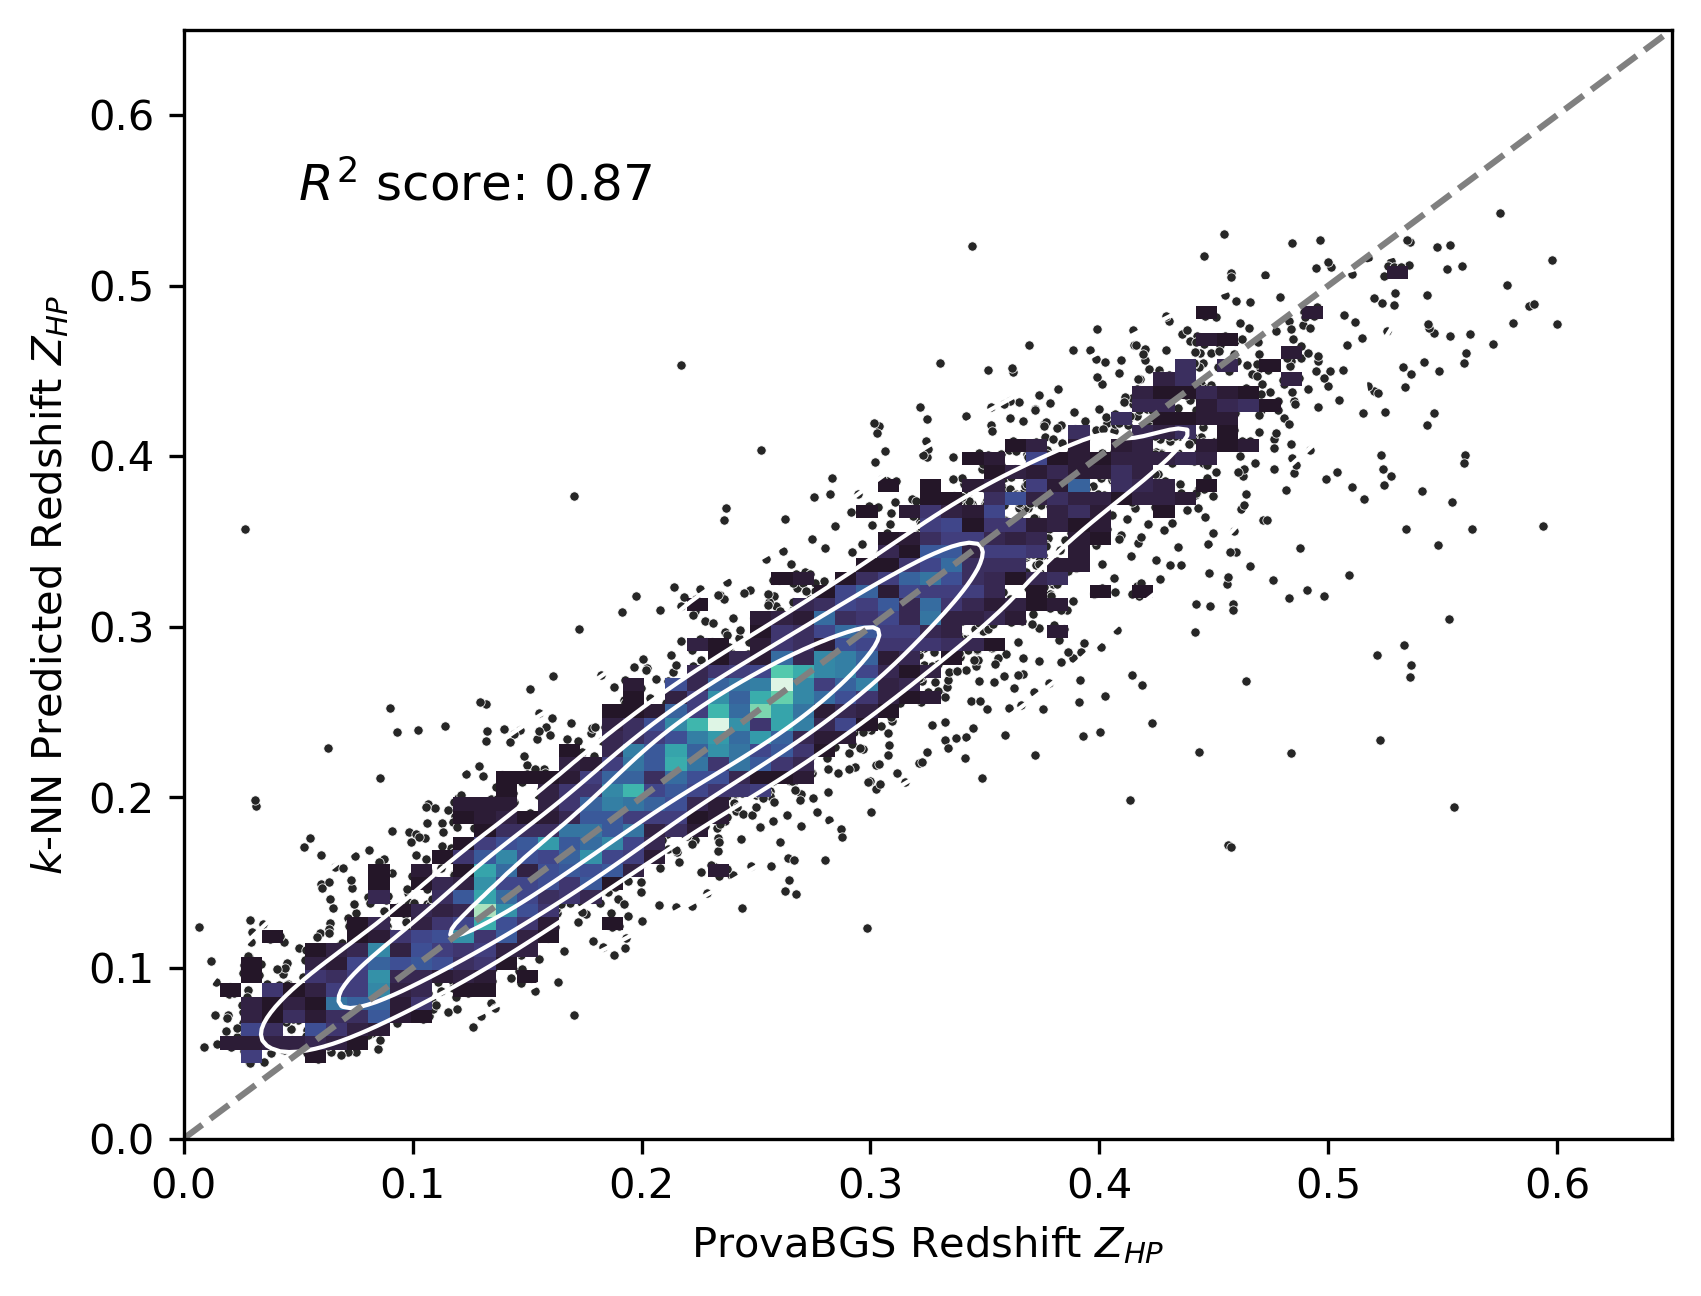
\includegraphics[width=\textwidth]{../figures/zeroshot_redshift_spectrum.png}
        \caption{Spectrum Embeddings for Redshift}
        \label{fig:redshift_spectrum}
    \end{subfigure}%
    \hfill
    \begin{subfigure}[b]{0.48\textwidth}
        \centering
        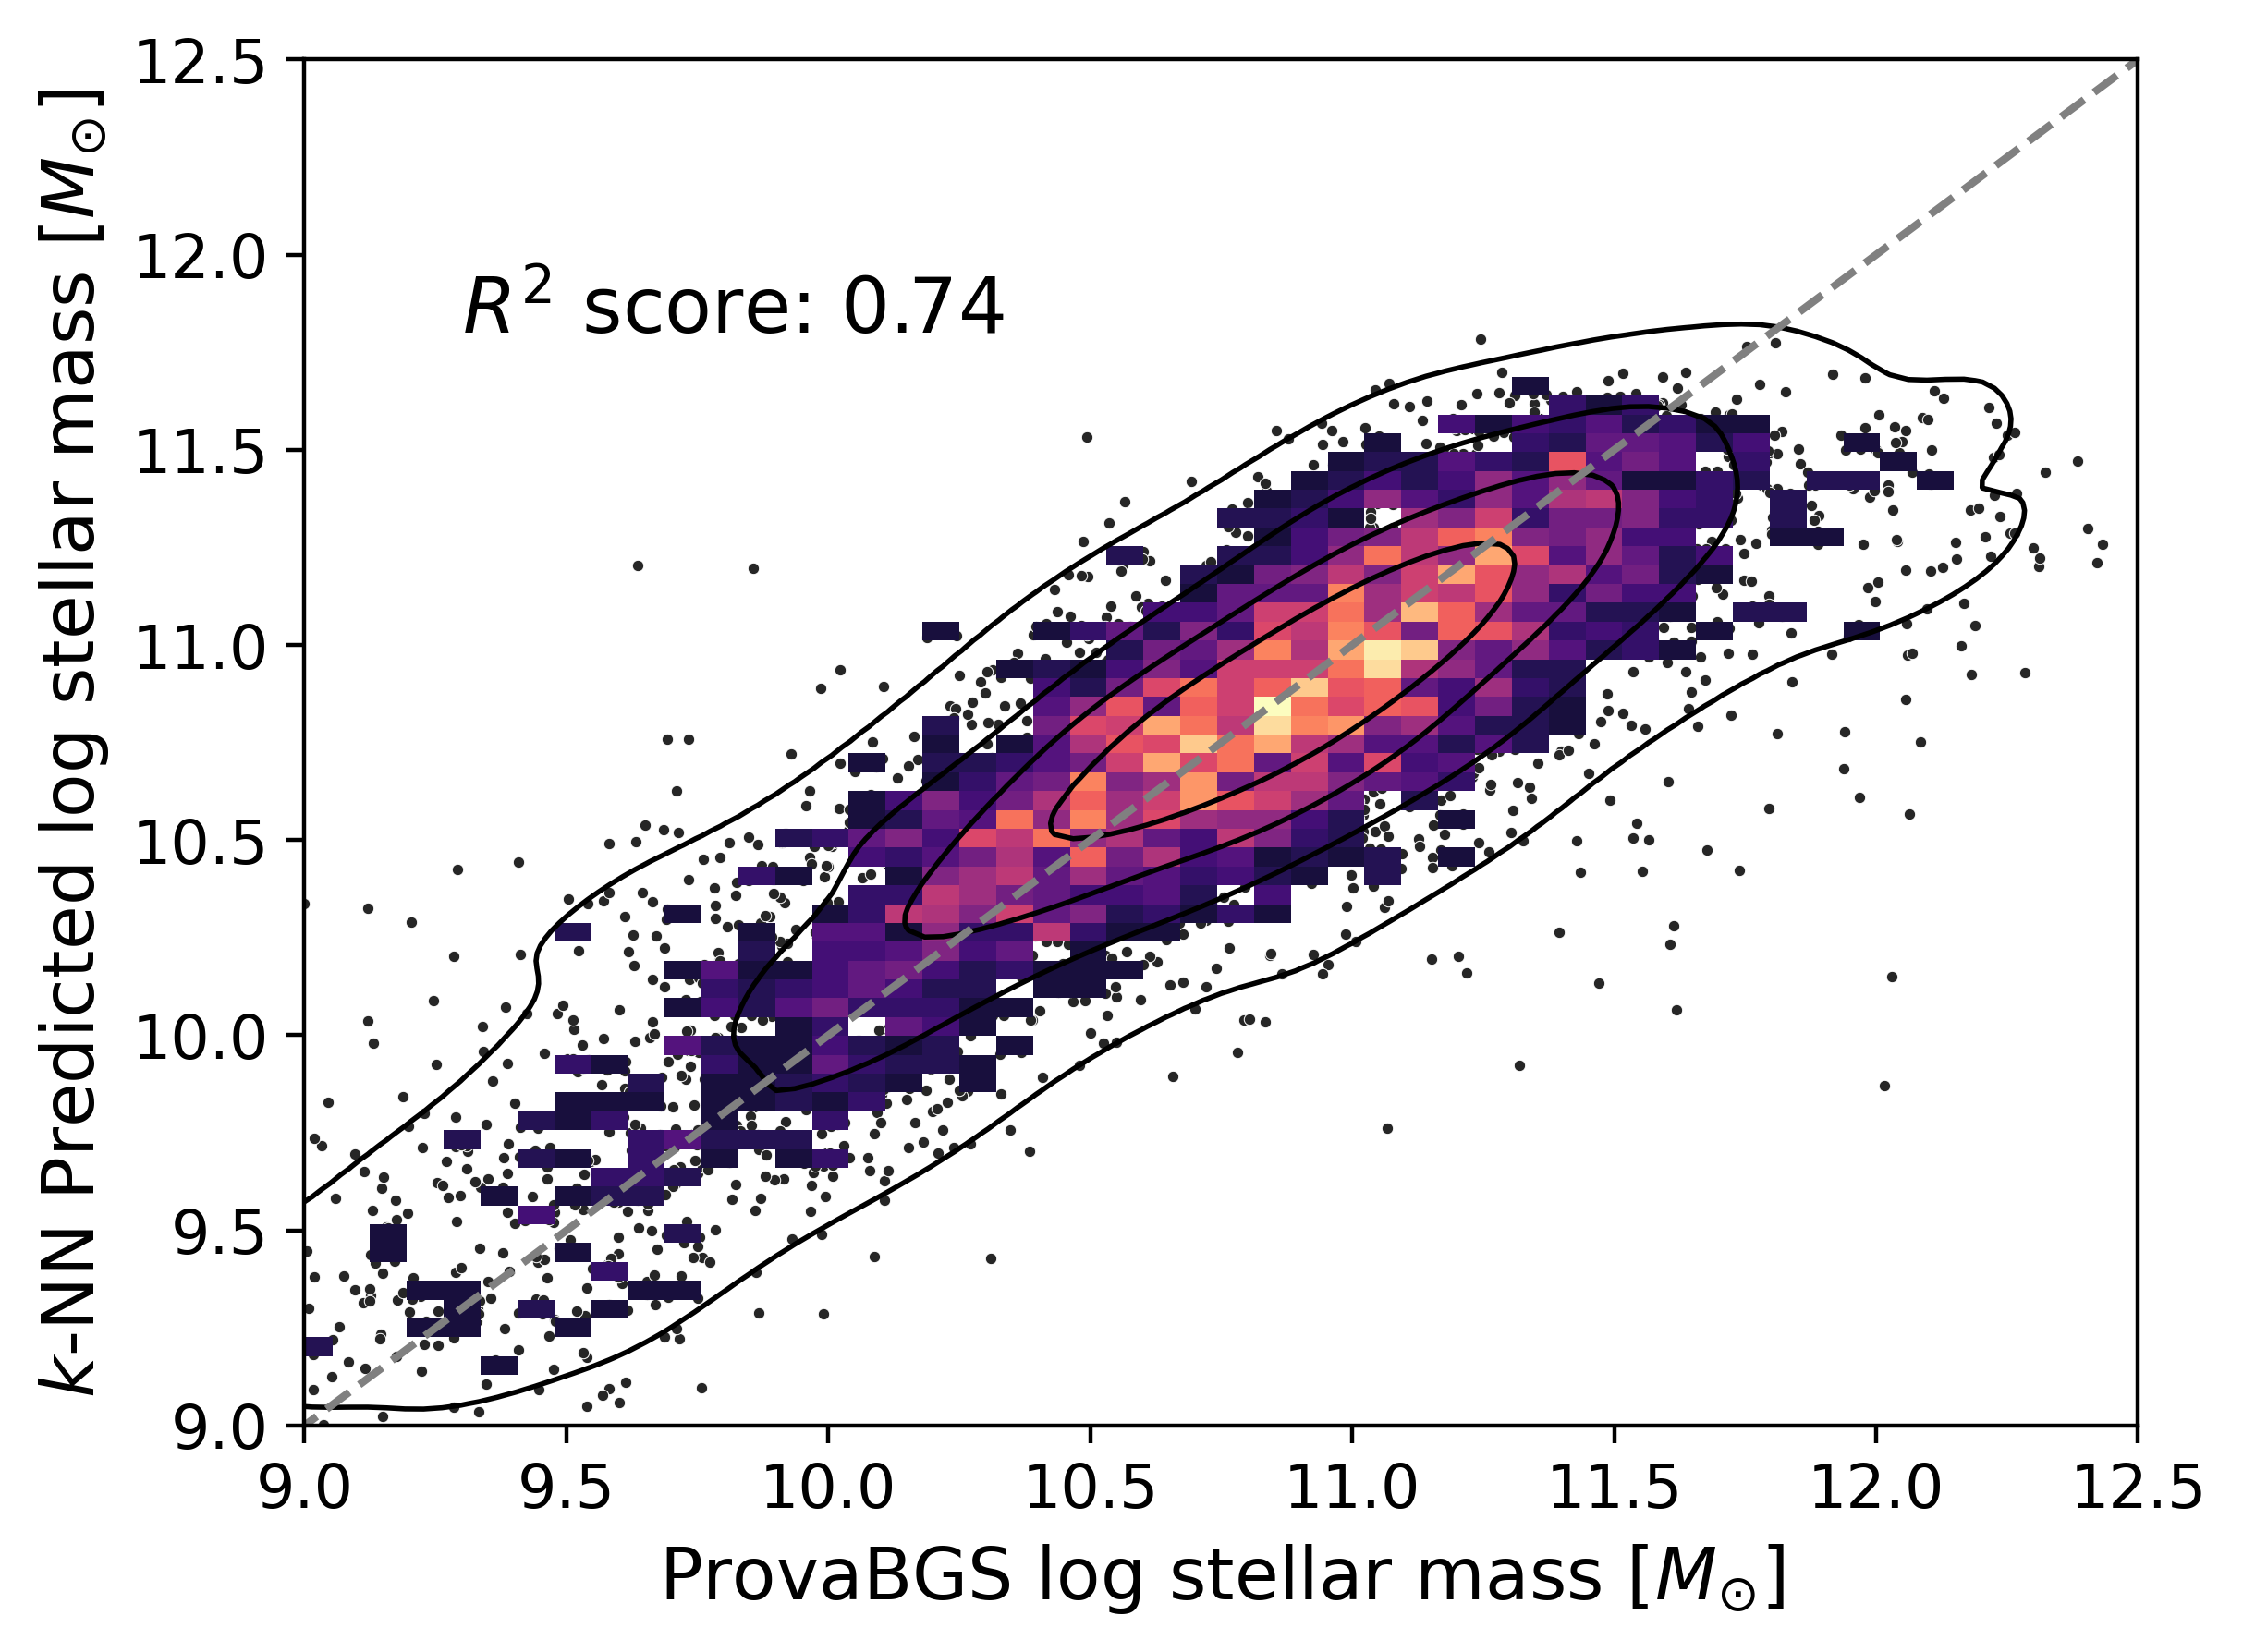
\includegraphics[width=\textwidth]{../figures/zeroshot_stellarmass_spectrum.png}
        \caption{Spectrum Embeddings for Stellar Mass}
        \label{fig:stellarmass_spectrum}
    \end{subfigure}

    % Row 3: Cross-Modal Embeddings
    \begin{subfigure}[b]{0.48\textwidth}
        \centering
        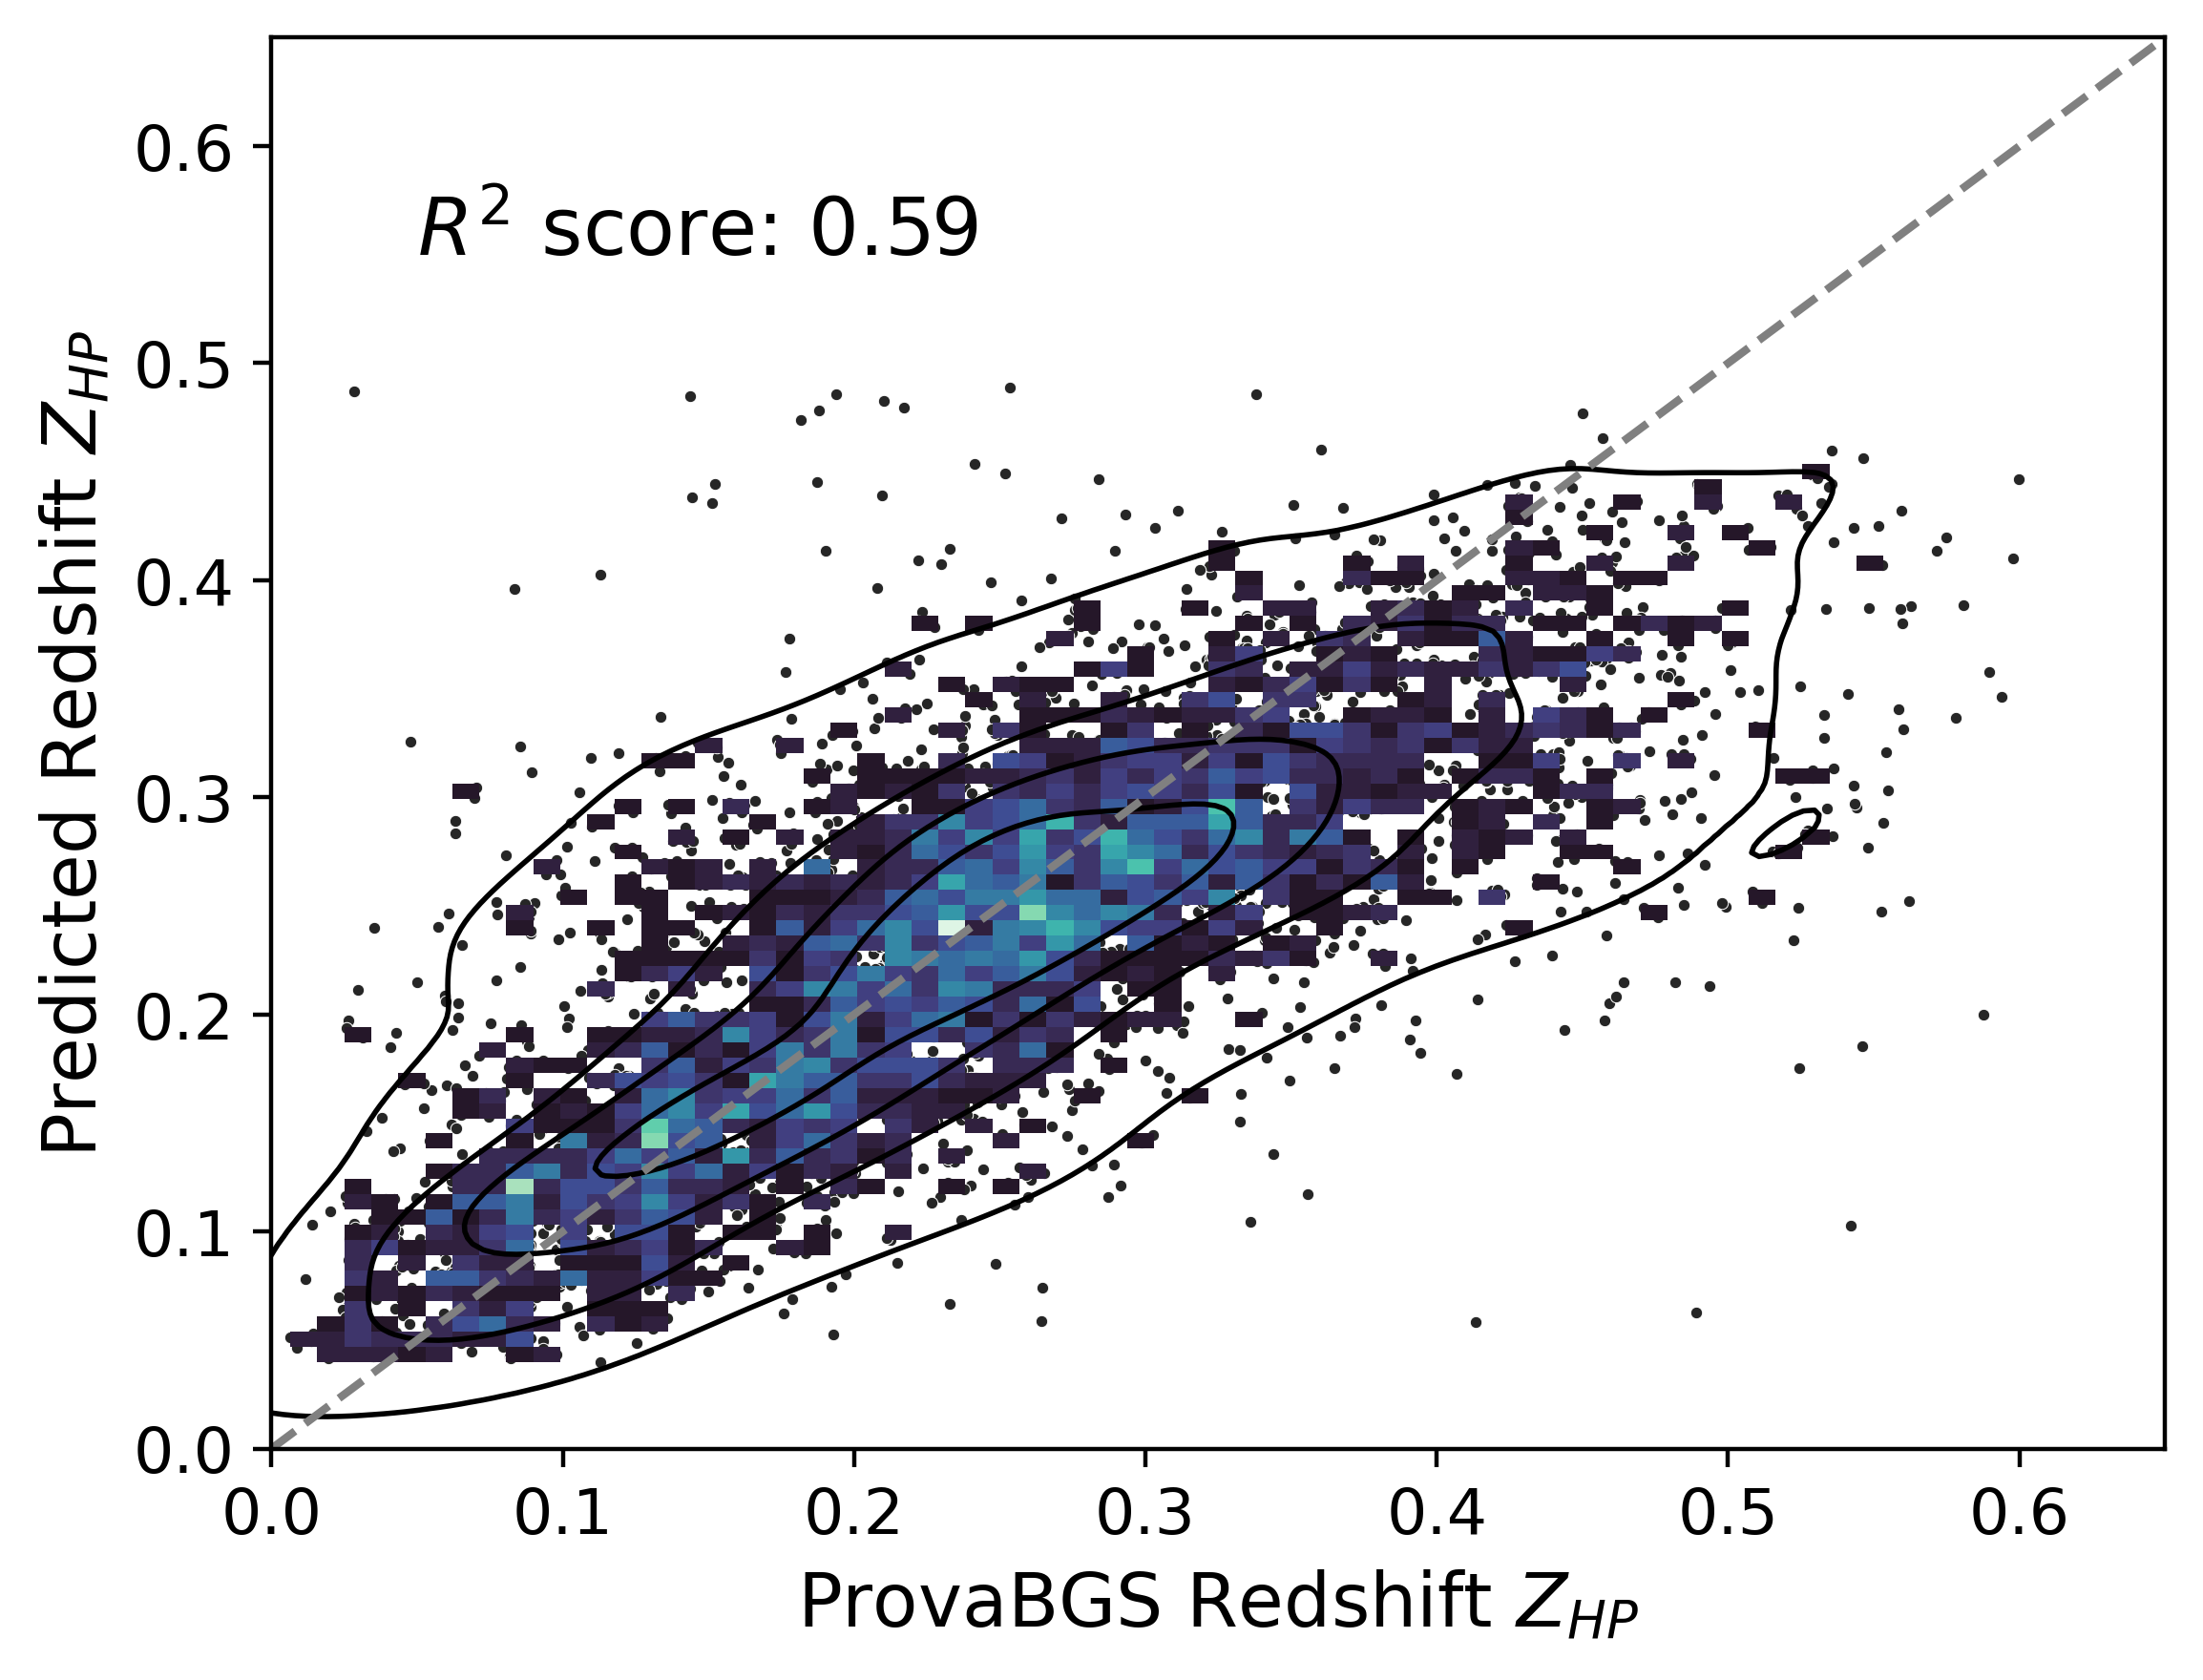
\includegraphics[width=\textwidth]{../figures/zeroshot_redshift_crossmodal.png}
        \caption{Cross-Modal Embeddings for Redshift}
        \label{fig:redshift_crossmodal}
    \end{subfigure}%
    \hfill
    \begin{subfigure}[b]{0.48\textwidth}
        \centering
        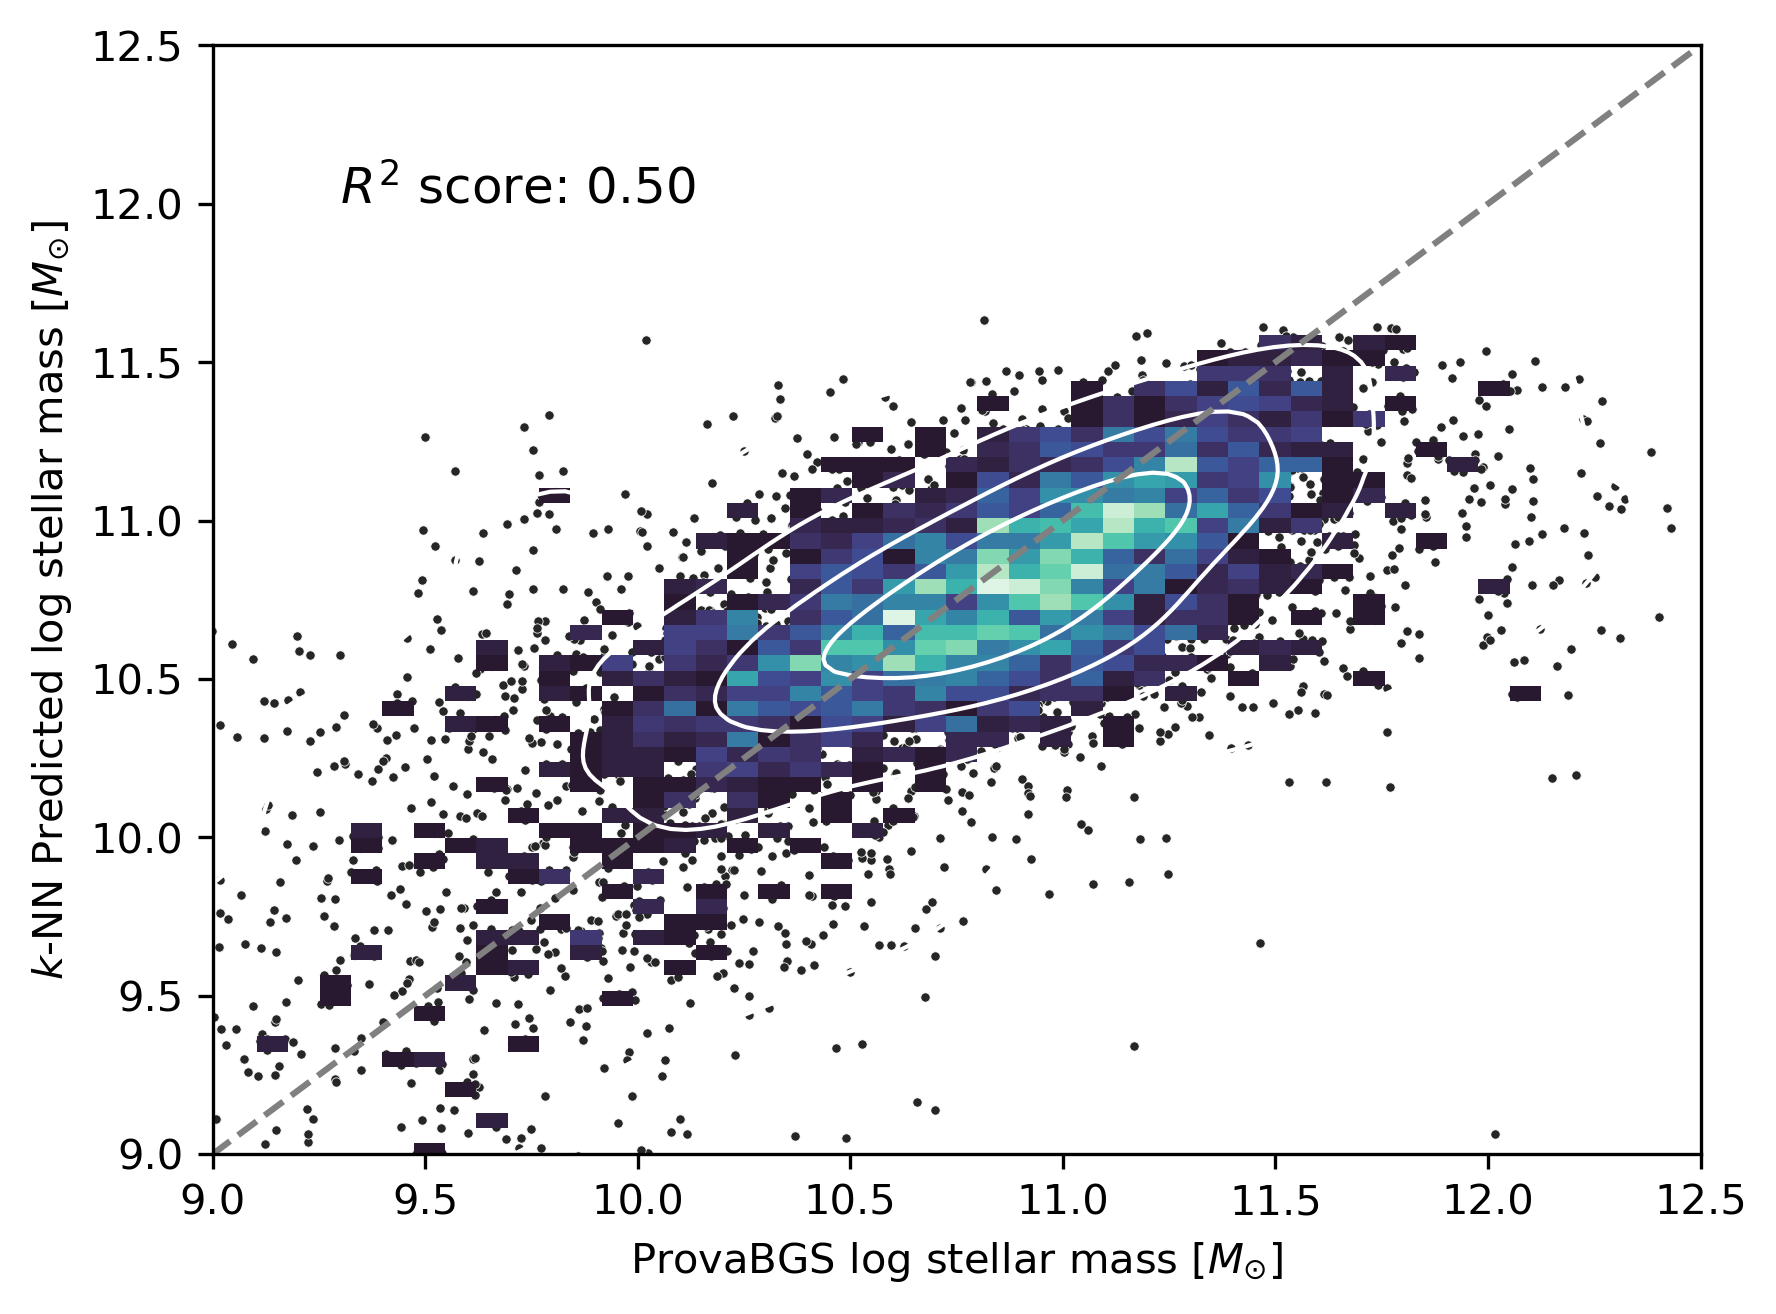
\includegraphics[width=\textwidth]{../figures/zeroshot_stellarmass_crossmodal.png}
        \caption{Cross-Modal Embeddings for Stellar Mass}
        \label{fig:stellarmass_crossmodal}
    \end{subfigure}

    \caption{Comparative visualizations of zero-shot redshift and stellar mass estimation across different embedding types.}
    \label{fig:zeroshot}
\end{figure}



\subsection{Embedding Space Clustering}
As an extension to the original work, we visualise the embedding space and subsequently use clustering techniques to further examine how the model structures the data. 

Fig.\ref{fig:umap_of_spectra} shows the UMAP projection of the spectrum embeddings, coloured by their catalogued redshift values $Z_{HP}$ on the left and stellar mass values $M_{\star}$ on the right. The projection reveals a clear structure, where low redshift galaxies are clustered in the lower left corner, rising to higher redshifts as we move to the upper right corner. The same pattern is present in the stellar mass plot. This again illustrates the emergent behaviour of the model to structure the embedding space around physically meaningful properties, despite not being explicitly trained on these properties. 


\begin{figure}[H]
    \centering
    \begin{adjustbox}{addcode={
      \begin{minipage}{\width}}{
      \end{minipage}},rotate=0,center}
      \includegraphics[width=1.15\textwidth]{../figures/umap_spectra_heatmap.png} % 1.3x text width to extend into the margins
    \end{adjustbox}
    \caption{UMAP projection of the spectrum embeddings coloured by redshift $Z_{HP}$ (left) and stellar mass $M_{\star}$ (right). The projection reveals a clear structure for both projections, where low redshift and stellar mass galaxies are clustered in the lower left corner, rising to higher values as we move to the upper right corner.}
    \label{fig:umap_of_spectra}
\end{figure}

\begin{figure}[H]
    \centering
    \begin{adjustbox}{addcode={
      \begin{minipage}{\width}}{
      \end{minipage}},rotate=0,center}
      \includegraphics[width=1.15\textwidth]{../figures/umap_image_heatmap.png} % 1.3x text width to extend into the margins
    \end{adjustbox}
    \caption{UMAP projection of the image embeddings coloured by redshift $Z_{HP}$ (left) and stellar mass $M_{\star}$ (right). The projection reveals a clear structure for both projections, where low redshift and stellar mass galaxies are clustered in the lower left corner, rising to higher values as we move to the upper right corner.}
    \label{fig:umap_of_images}
\end{figure}


\begin{figure}[H]
    \centering
    \begin{adjustbox}{addcode={
      \begin{minipage}{\width}}{
      \end{minipage}},rotate=0,center}
      \includegraphics[width=1.15\textwidth]{../figures/umap_both_heatmap.png}
    \end{adjustbox}
    \caption{UMAP projection of the image embeddings coloured by redshift $Z_{HP}$ (left) and stellar mass $M_{\star}$ (right). The projection reveals a clear structure for both projections, where low redshift and stellar mass galaxies are clustered in the lower left corner, rising to higher values as we move to the upper right corner.}
    \label{fig:umap_of_both}
\end{figure}

Fig.\ref{fig:umap_of_images} and Fig.\ref{fig:umap_of_both} show the UMAP projection of the image embeddings and the combined image-spectrum embeddings, respectively. Similarly to the spectrum embeddings, we again see this clear structuring in the embedding space, with one difference: these mapping include a large `island' of galaxies that does not contain particular property values. Rather, it largely follows a similar pattern to the main `island', indicating this break-off is caused by some other property.


% To further examine this and other potential islands, we use DBScan to directly cluster the UMAP projection. The clusters are illustrated in Fig.\ref{fig:umap_DBSCAN}

% \begin{figure}[H]
%     \centering
%     \begin{adjustbox}{addcode={
%       \begin{minipage}{\width}}{
%       \end{minipage}},rotate=0,center}
%       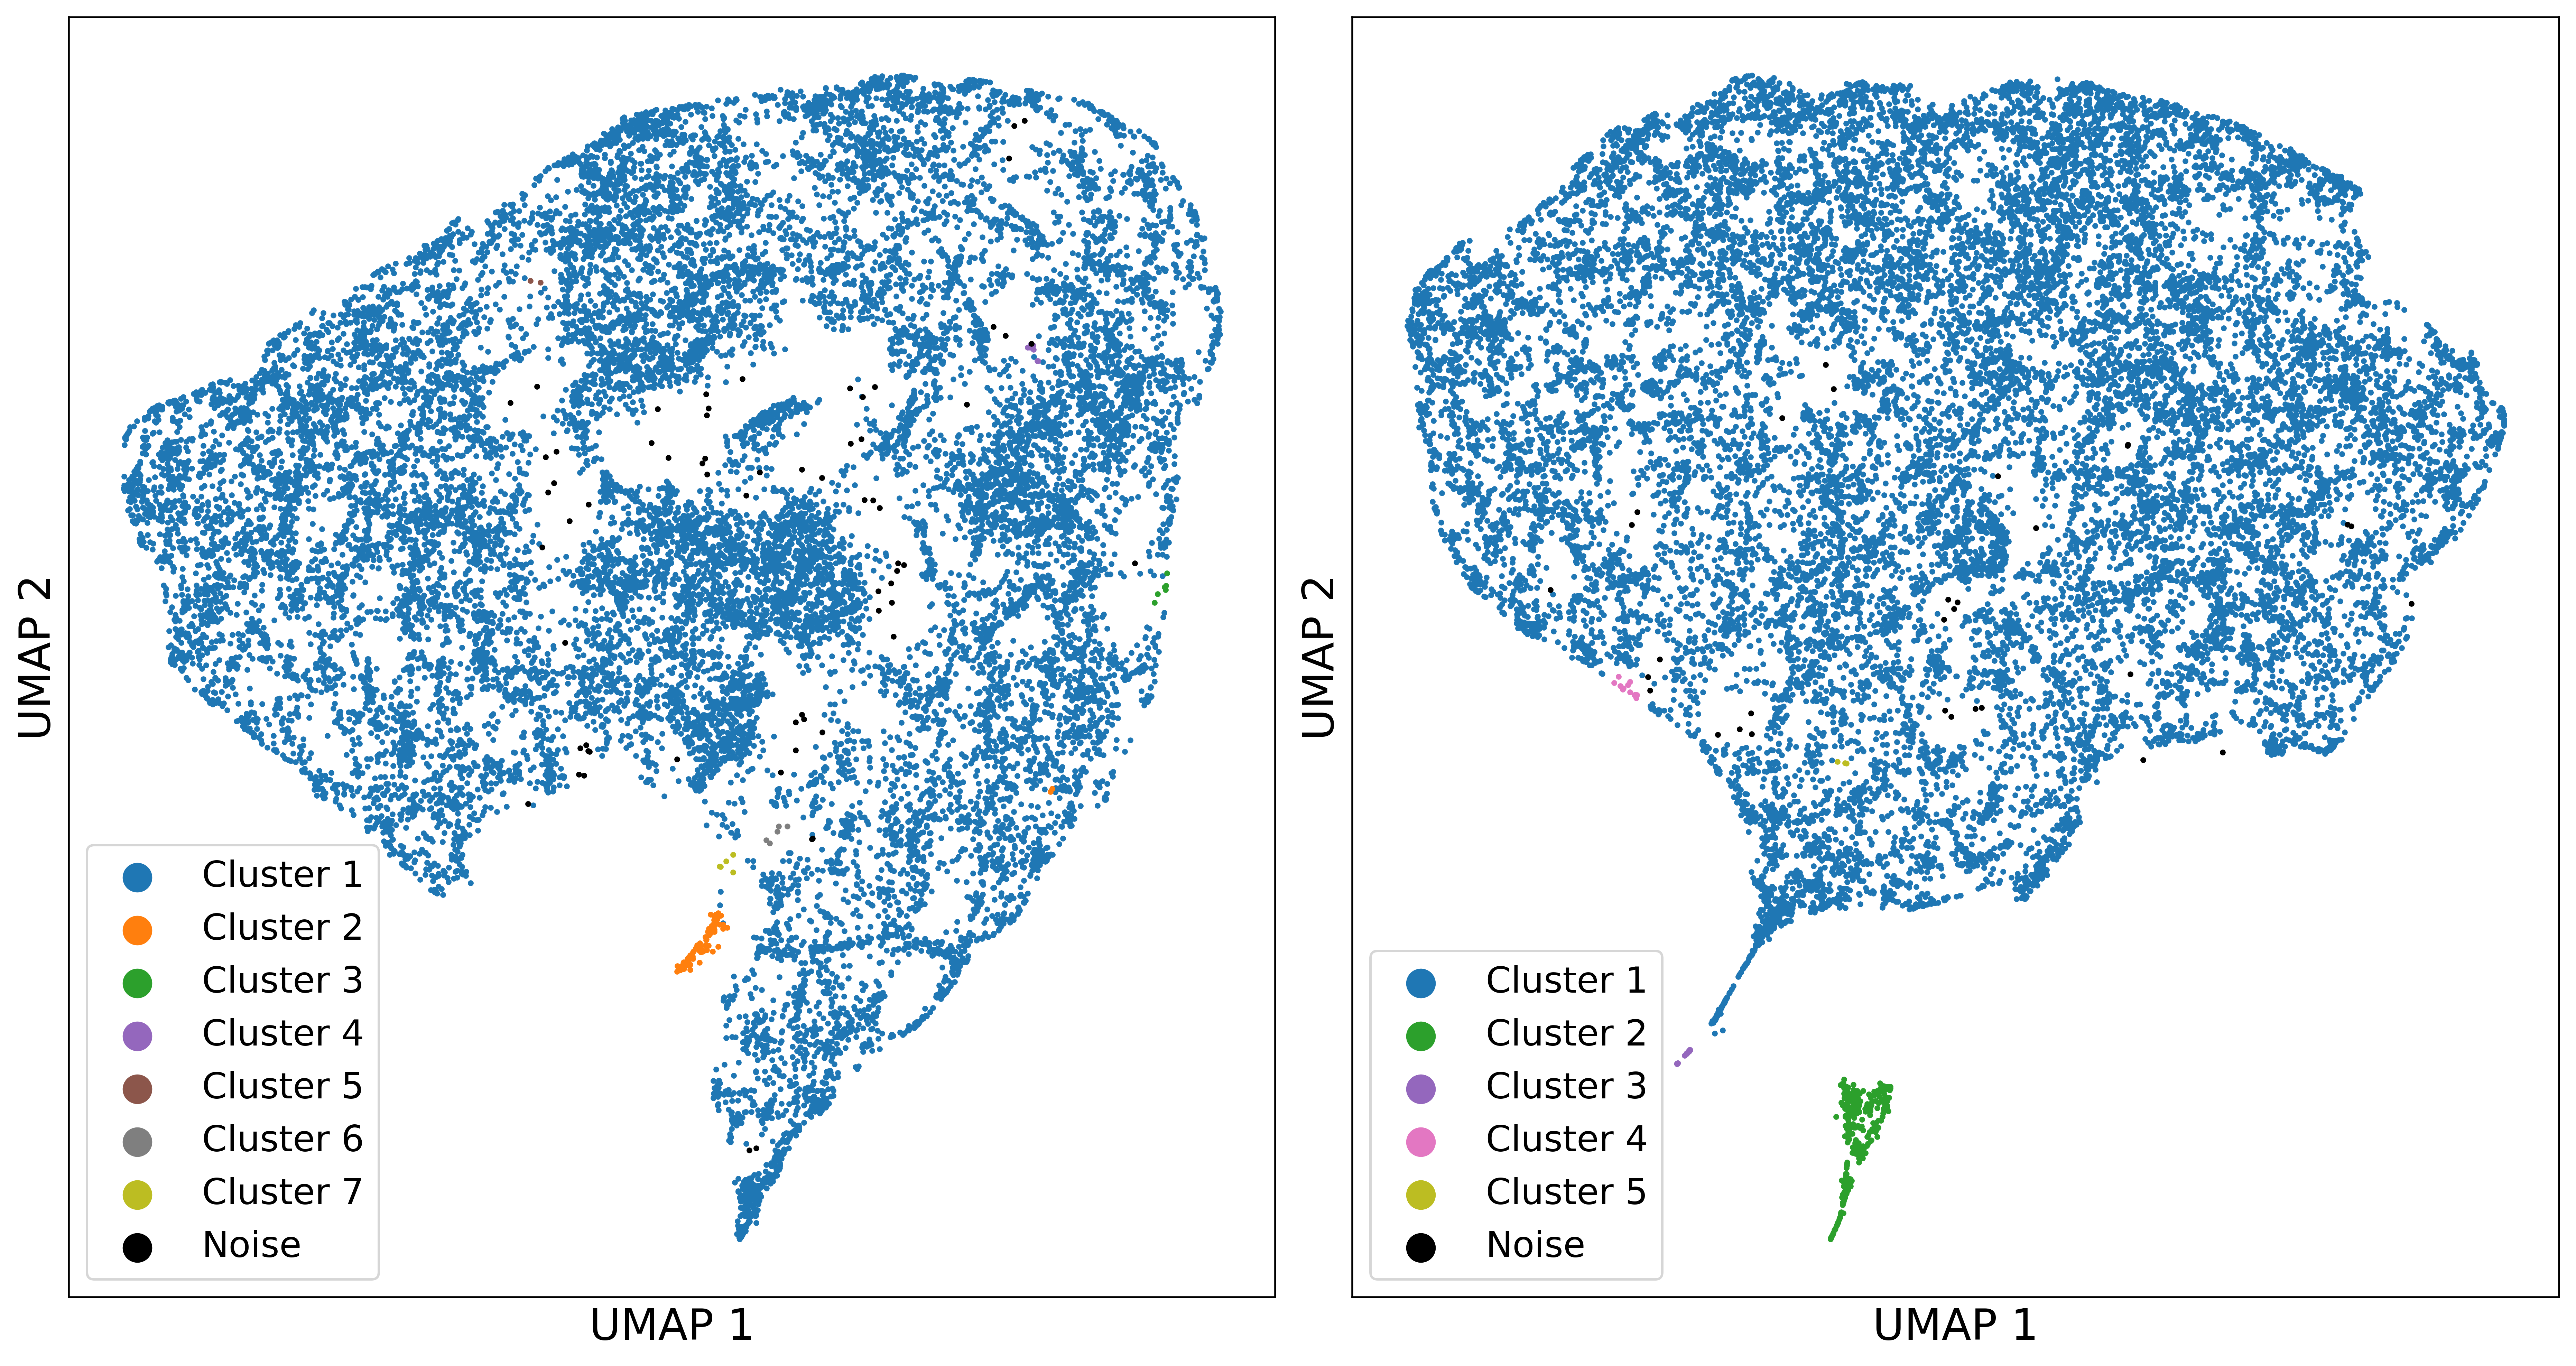
\includegraphics[width=1.15\textwidth]{../figures/umap_dbscan_clusters.png}
%     \end{adjustbox}
%     \caption{UMAP projection of the spectrum embeddings (left) and image embeddings (right) coloured by the DBScan clustering.}
%     \label{fig:umap_DBSCAN}
% \end{figure}

To further examine this and other potential islands, we use DBScan to directly cluster the UMAP projection of the image embeddings. We set $\epsilon = 0.20$ and the minimum number of samples to 5. These were chosen by trial and error to produce a reasonable number of clusters in both the image and spectrum embeddings, with a reasonable number of galaxies in each. We then draw sample galaxies for each cluster to visually inspect. The clusters for the image embeddings are illustrated in Fig.\ref{fig:umap_DBSCAN}.

We reveal that the image embedder has successfully separated galaxy images that contain artifacts such as [fix] into a distinct embedding island (Cluster 2). The galaxies contained in those images have variable redshifts and stellar masses, and are follow the same distribution as the main island. We further display 3 more islands. This is potentially a useful feature for quickly identifying artifacts in galaxy catalogues. Cluster 3 and 4 contain galaxies that largely fill the image, are mostly spiral and have high brightness. This indicates that model is able to separate galaxies based on their morphology, which is a key feature in galaxy classification. It is important to note that although we are looking at the image embeddings, these are informed by the spectrum embeddings, which means that it contains information about the galaxy's spectrum as well.


\begin{figure}[H]
    \centering
    \begin{adjustbox}{addcode={
      \begin{minipage}{\width}}{
      \end{minipage}},rotate=0,center}
      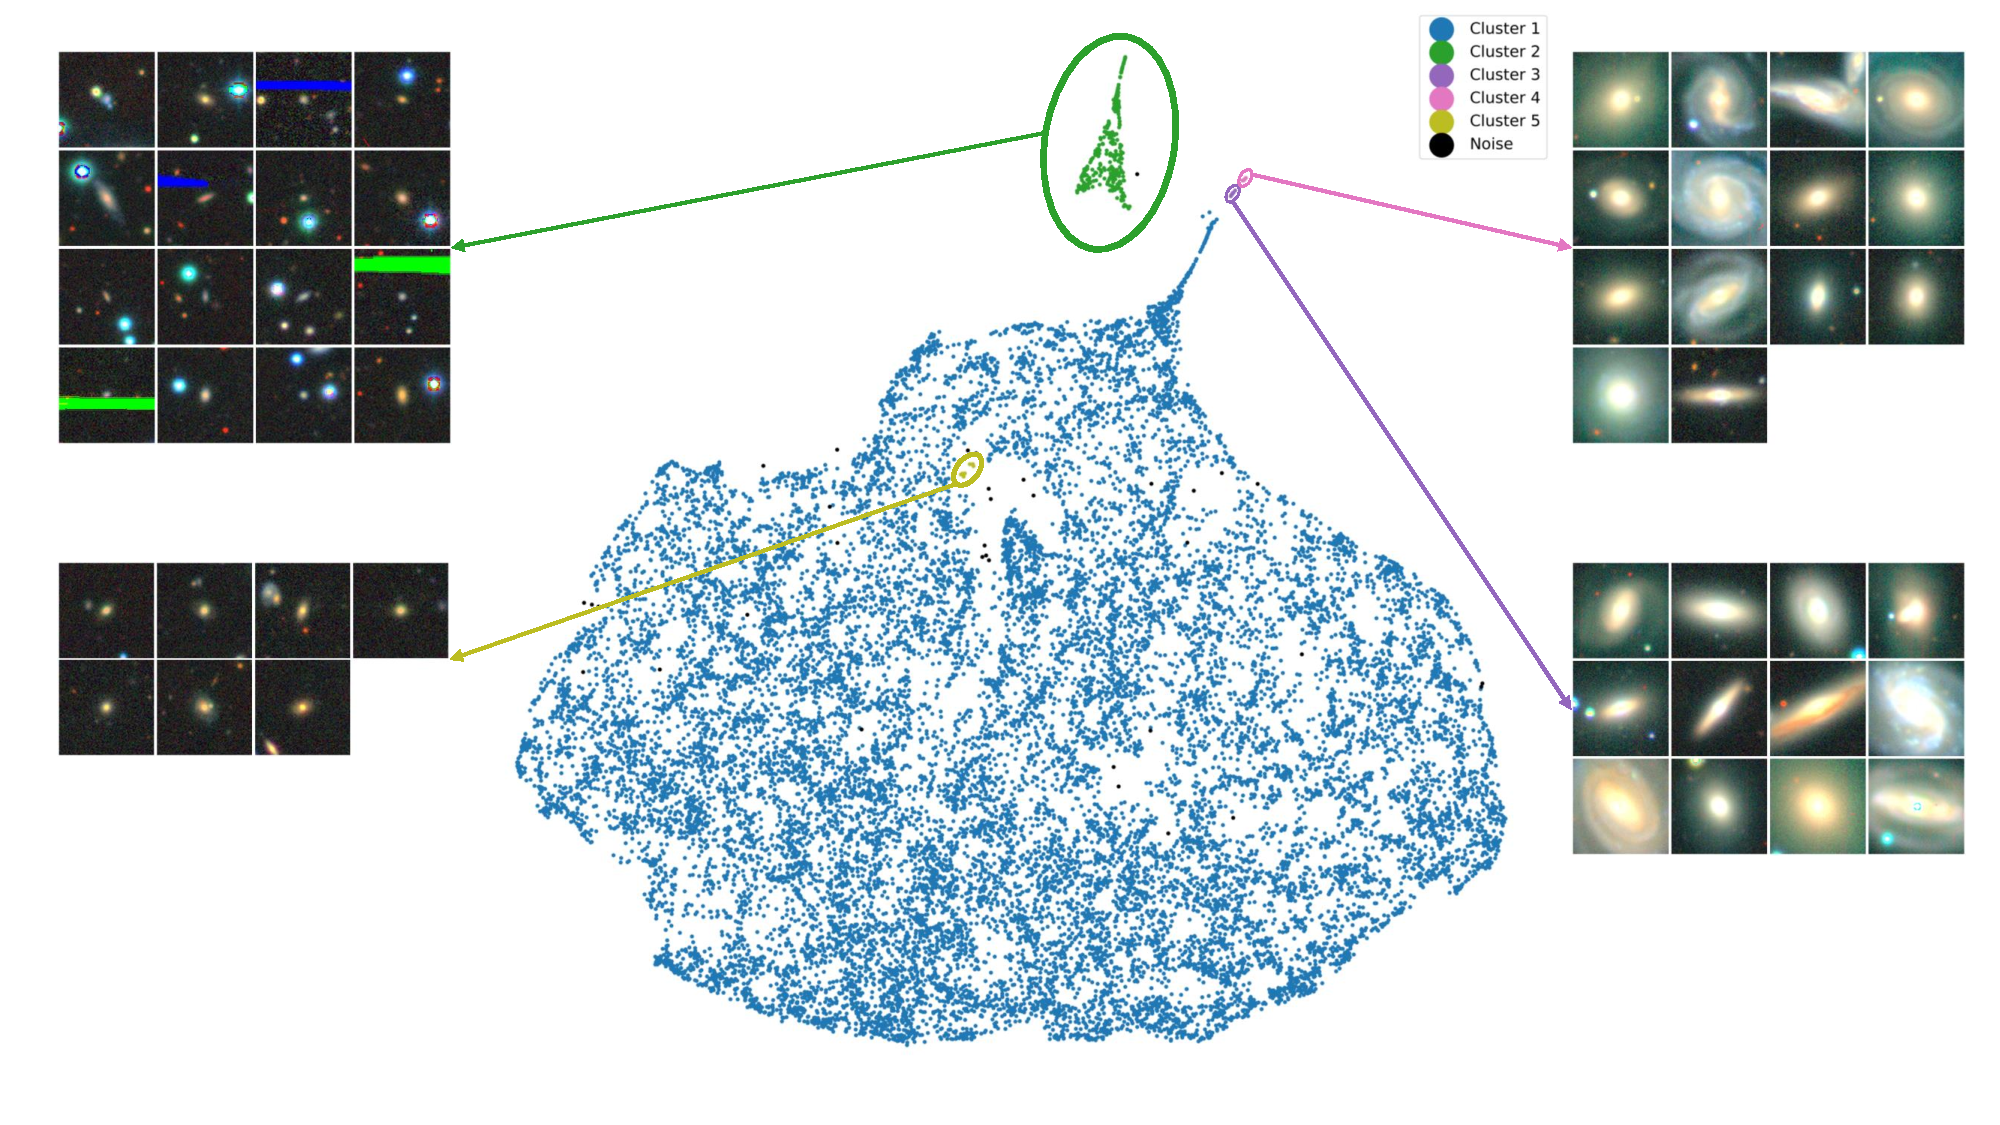
\includegraphics[width=1.15\textwidth]{../figures/dbscan_image_clusters_shown.pdf}
    \end{adjustbox}
    \caption{UMAP projection of the image embeddings coloured by the DBScan clustering.}
    \label{fig:umap_DBSCAN}
\end{figure}


It is important to note that although we visualise the embeddings of one modality in isolation, their structuring is informed by the other modality during contrastive training. We illustrate this statement by showcasing the results of $k$-Means clustering on the full dimensional space of just the spectrum embeddings. Here, we first perform the clustering and then project the clusters onto the UMAP projection of the spectrum embeddings. We choose to use 10 clusters, as they yield a reasonable silhouette score and a reasonable number of galaxies in each cluster. 

We then visualise a random sample of the spectra in each cluster, as shown in Fig.\ref{fig:annotated_spectra}. We observe that galaxies in the same cluster follow similar trends in their spectra, both in terms of the overall shape, the presense of specific spectral features and the flux range and scale. In addition to this we show that not only are the spectra in the same cluster similar, but the images of the galaxies are also visually similar, as shown in Fig.\ref{fig:annotated_images}. Recall that we are only considering the spectrum embeddings in this case, which means that the model has learned to structure the spectrum embeddings in a way that is informed by the image embeddings. This is a key feature of the AstroCLIP model, as it allows for the alignment of the two modalities in the shared latent space.





\begin{figure}[H]
    \centering
    \begin{adjustbox}{addcode={
      \begin{minipage}{\width}}{
      \end{minipage}},rotate=0,center}
      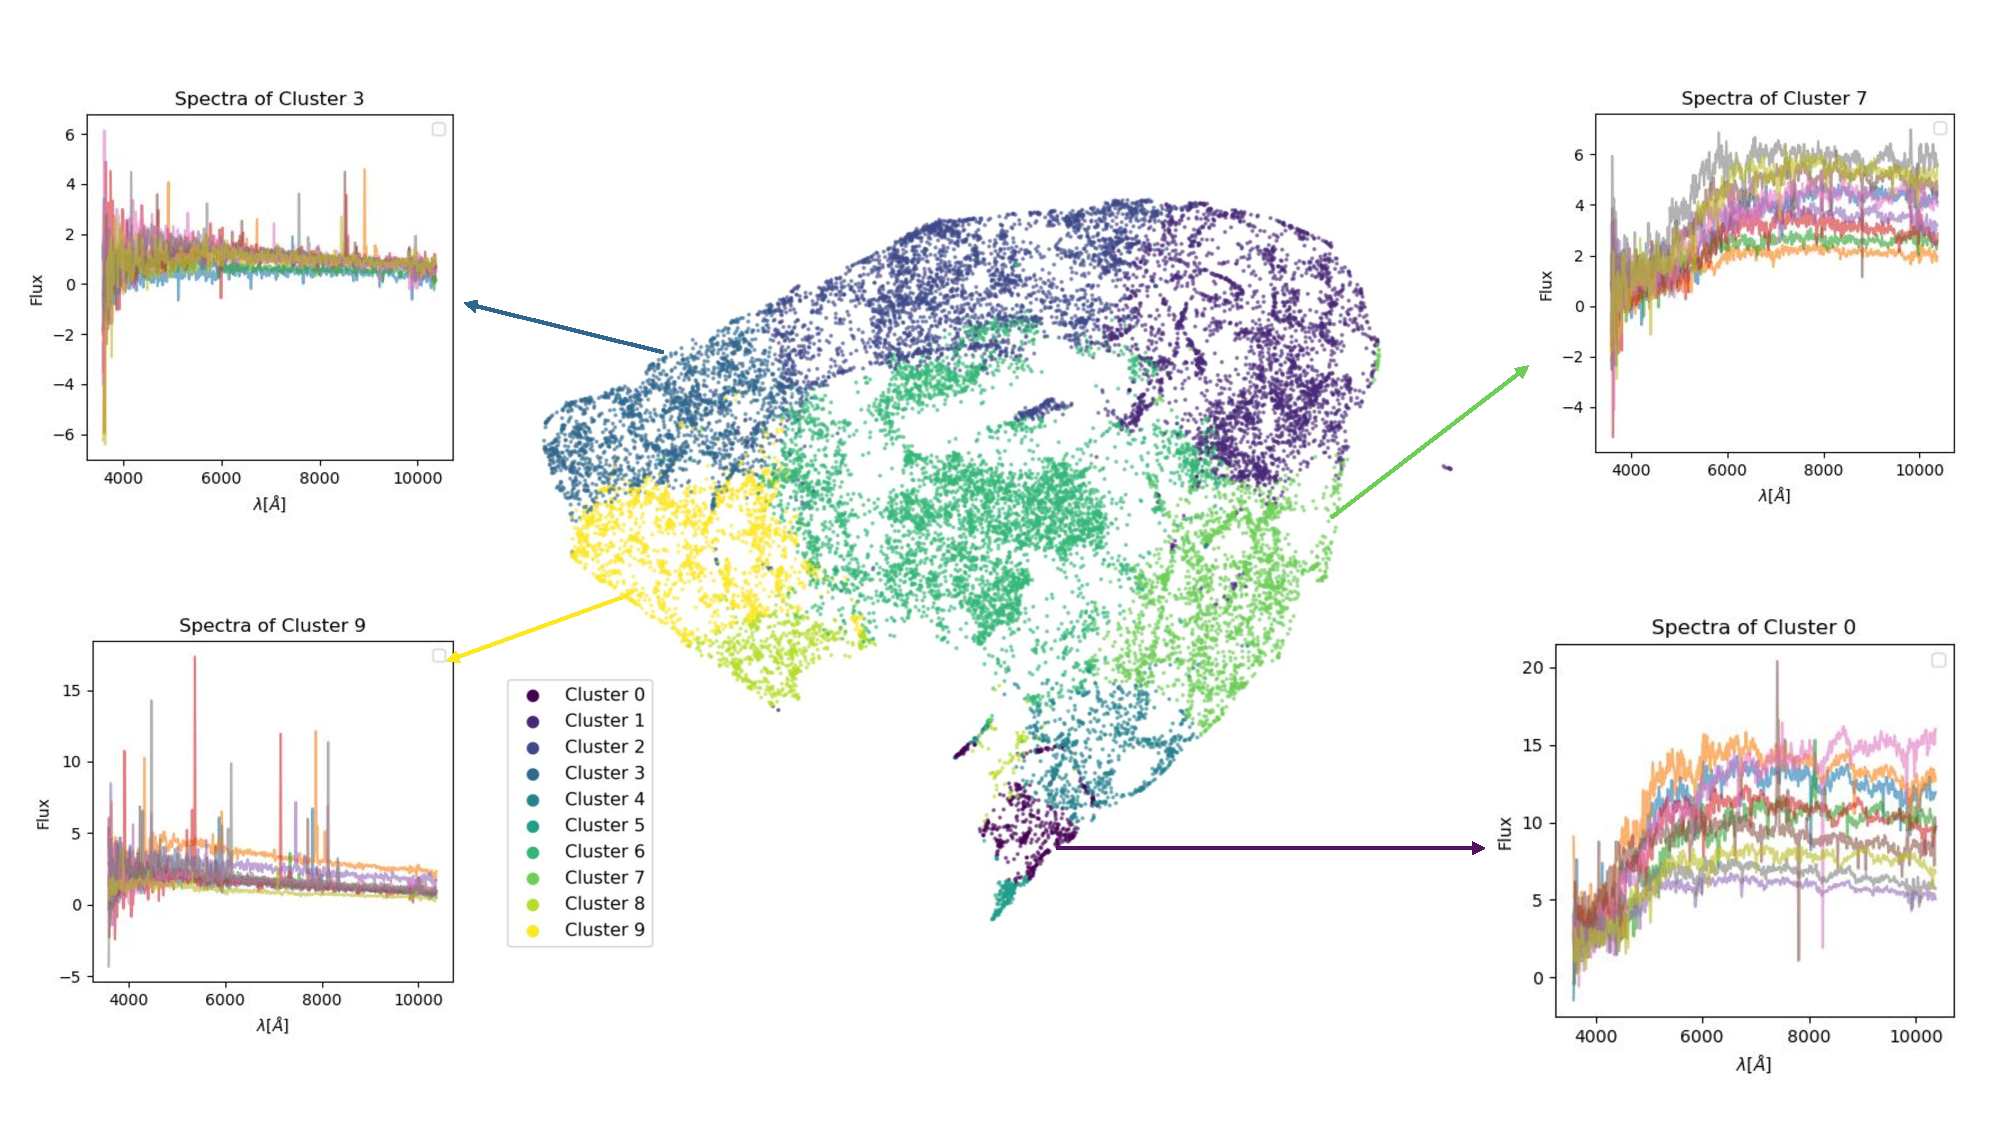
\includegraphics[width=1.15\textwidth]{../figures/umap_spectrum_annotated_spectra.pdf}
    \end{adjustbox}
    \caption{UMAP projection of the image embeddings coloured by the DBScan clustering.}
    \label{fig:annotated_spectra}
\end{figure}

\begin{figure}[H]
    \centering
    \begin{adjustbox}{addcode={
      \begin{minipage}{\width}}{
      \end{minipage}},rotate=0,center}
      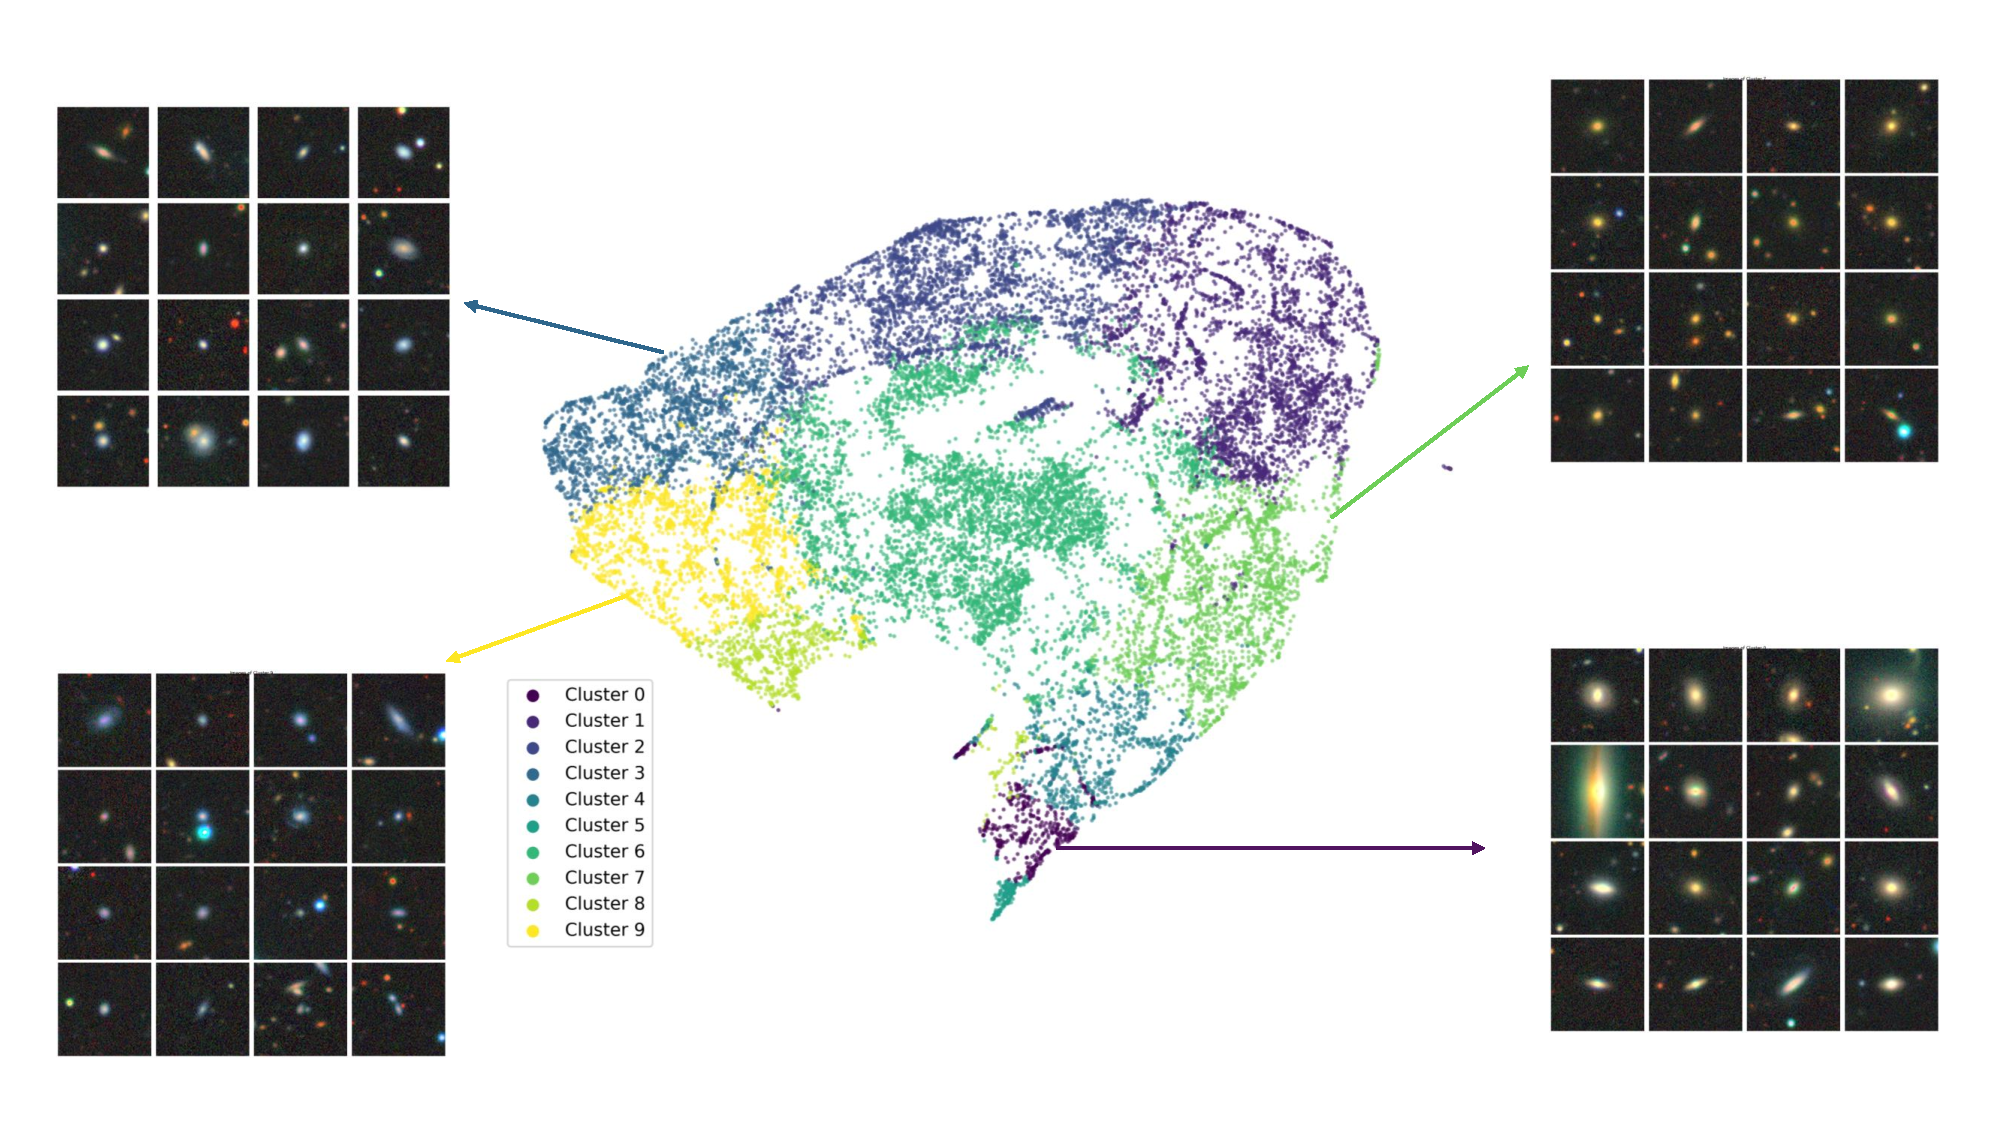
\includegraphics[width=1.15\textwidth]{../figures/umap_spectrum_annotated_images.pdf}
    \end{adjustbox}
    \caption{UMAP projection of the image embeddings coloured by the DBScan clustering.}
    \label{fig:annotated_images}
\end{figure}









\newpage
\bibliographystyle{unsrt}
\bibliography{references.bib}

\end{document}